\documentclass[a4paper,11pt]{scrartcl}
\usepackage{graphicx}
\usepackage[utf8]{inputenc} %-- pour utiliser des accents en français
\usepackage{amsmath,amssymb,amsthm} 
\usepackage[round]{natbib}
\usepackage{url}
\usepackage{xspace}
\usepackage[left=20mm,top=20mm]{geometry}
\usepackage{algorithmic}
\usepackage{subcaption}
\usepackage{mathpazo}
\usepackage{booktabs}
\usepackage{hyperref}
\usepackage{float}
% \usepackage{draftwatermark}


\title{Analyse de Performance}
\author{Barona Stephanie, Grand Maxence}
\date{\today}


\begin{document}

\maketitle

%%%
%
\section{Introduction}
\subsection{Environnement}
\begin{itemize}
\item OS : Xubuntu
\item 4 processeurs Intel(R) Core(TM) i5-3470 CPU 3.20 GHz
\item La machin est branché sur un r\'eseau des probl\`emes au niveau du r\'eseau peuvent poser des probl\`emes de performance.
\item Mis \`a part les processus utilis\'es par le kernel, sur lesquels nous n'avons pas la main, nous n'avons laisser que l'ex\'ecution des programmes. Aucune application ou autre programme tourne en m\^{e}me temps que notre jeu de tests
\end{itemize}
\subsection{Jeu de Tests et Hypoth\`eses}
Nous avons tester l'algorithme s\'equentiel de tri, ainsi que l'algorithme parall\`ele de tri. Pour l'algorithme parall\`ele de tri, nous avons test\'e avec un nombre de threads variant de 2 \`a 16. Chaque algorithme \`a \'et\'e test\'e sur diff\'erents vecteurs, de tailles variant de 1000 \`a 1000000 (avec un pas de 2500). Chaque tests \`a \'et\'e refait 30 nfois pour \'eliminer les incercitudes de mesures. A chaque tests nous avons calcul\'e le temps d'ex\'ecution de l'algorithme, ainsi que le temps CPU  cumul\'e de l'utilisateur.\\Nous avons ensuite calcul\'e l'acc\'eleration de chaque version de l'algorithme parall\`ele par rapport \`a l'algorithme s\'equantiel : $a = \frac{T_{seq}}{T_{par}} $. Nous prenons l'hypoth\`ese que l'acc\'el\'eration de Temps machine sera sup\'erieur \`a un pour tous les algorithmes paral\`elle, car nous supposons que plus il y aura de thread, plus l'ex\'ecution sera rapide. Nous prenons aussi l'hypoth\`ese que cette acc\'el\'eration sera la plus forte pour 4 threads, car nous avons test\'e sur une machine \`a 4 processeurs. Pour le temps cpu de l'utilisateur, nous prenons l'hyporth\`ese que ce temps augmentera avec le nombre de thread, nous supposons donc que l'acc\'el\'eration sera inf\'erieur \`a un.\\
Nous avons ensuite calcul\' l'efficacit\'e : $e = \frac{a}{NB_{proc}}$

\section{Avec 2 threads}
\subsection{Temps d'ex\'ecution}

\begin{figure}[H] \center
   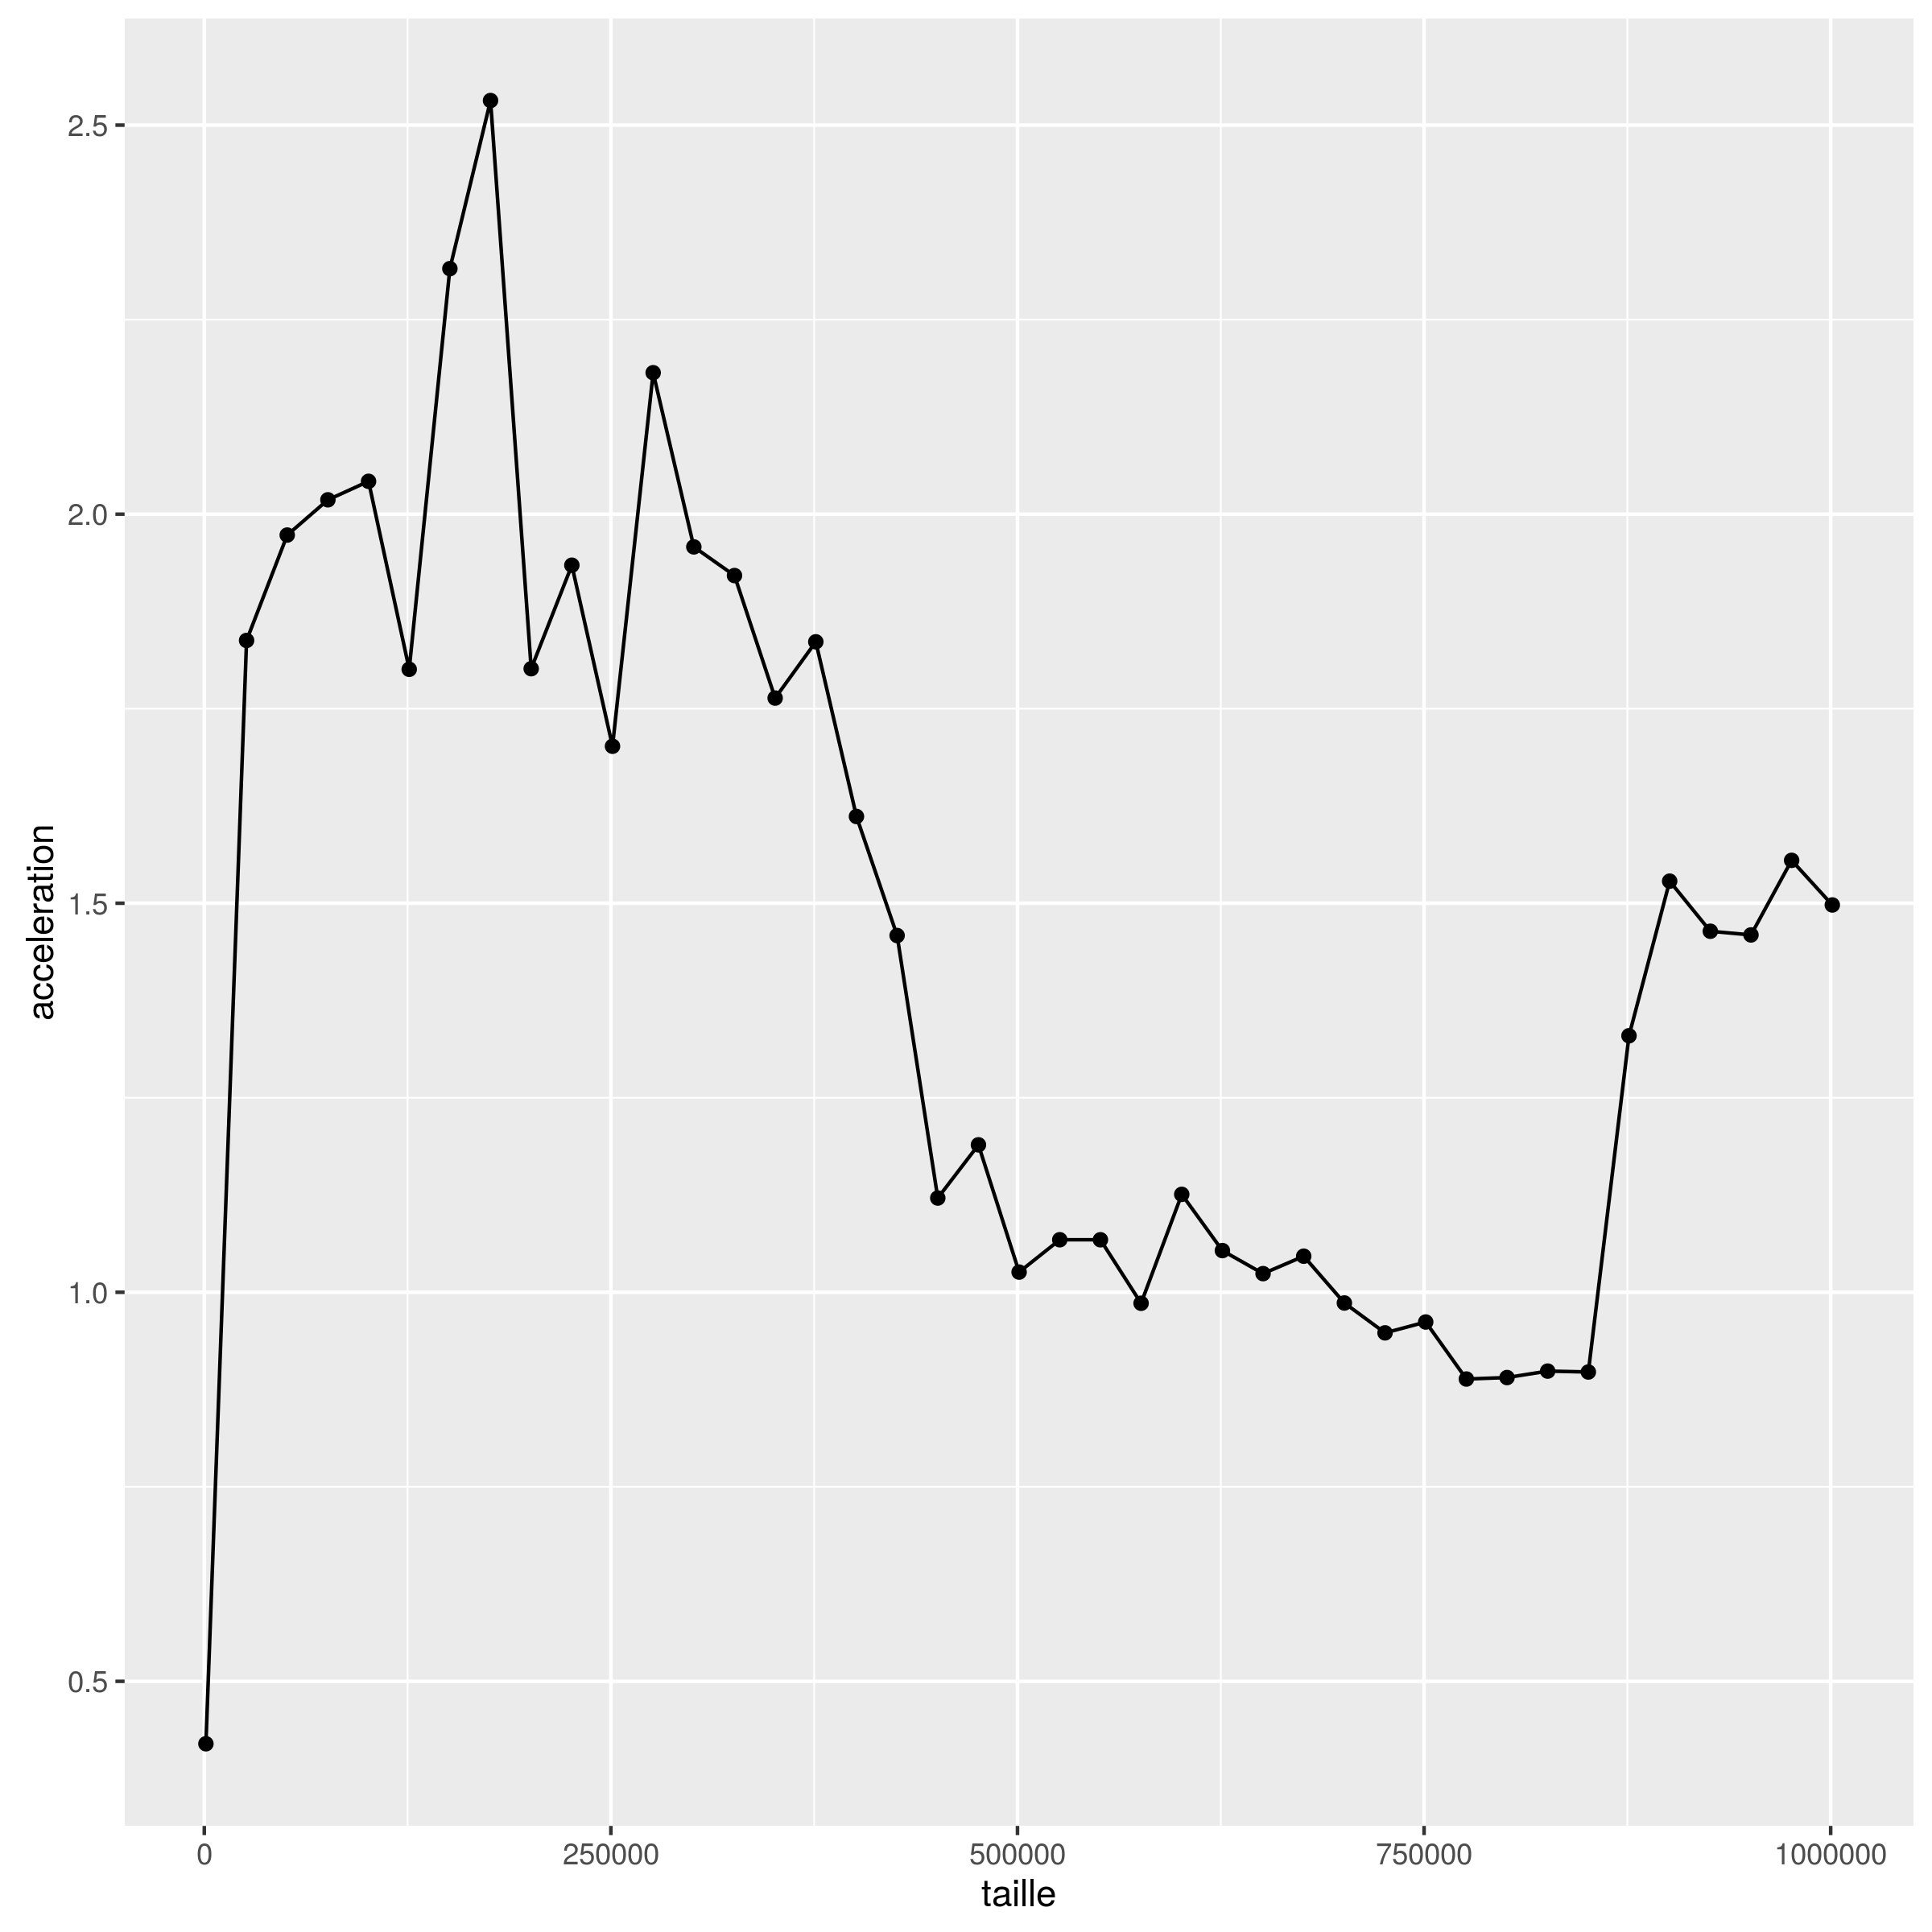
\includegraphics[scale=0.5] {graphes/global_temps_machine_accel2.png}
\end{figure}

Nous observons que pour des vecteurs allant d'une taille de 1000 \'el\'ements \`a 1000000 d'\'el\'ements, l'acc\'el\'eration est toujours sup\'erieur \`a 1. Nous observons aussi que l'acc\'el\'eration est la plus grande, pour des vecteurs d'une taille d'environ 200000 \'el\'ements. Pass\'e ce seuil, le niveau de l'acc\'el\'eration baisse et finit par tendre vers un, pass\' le seuil des 700000 \'el\'ements.   


\subsection{Temps CPU cumul\'e de l'utilisateur}
\begin{figure}[H] \center
   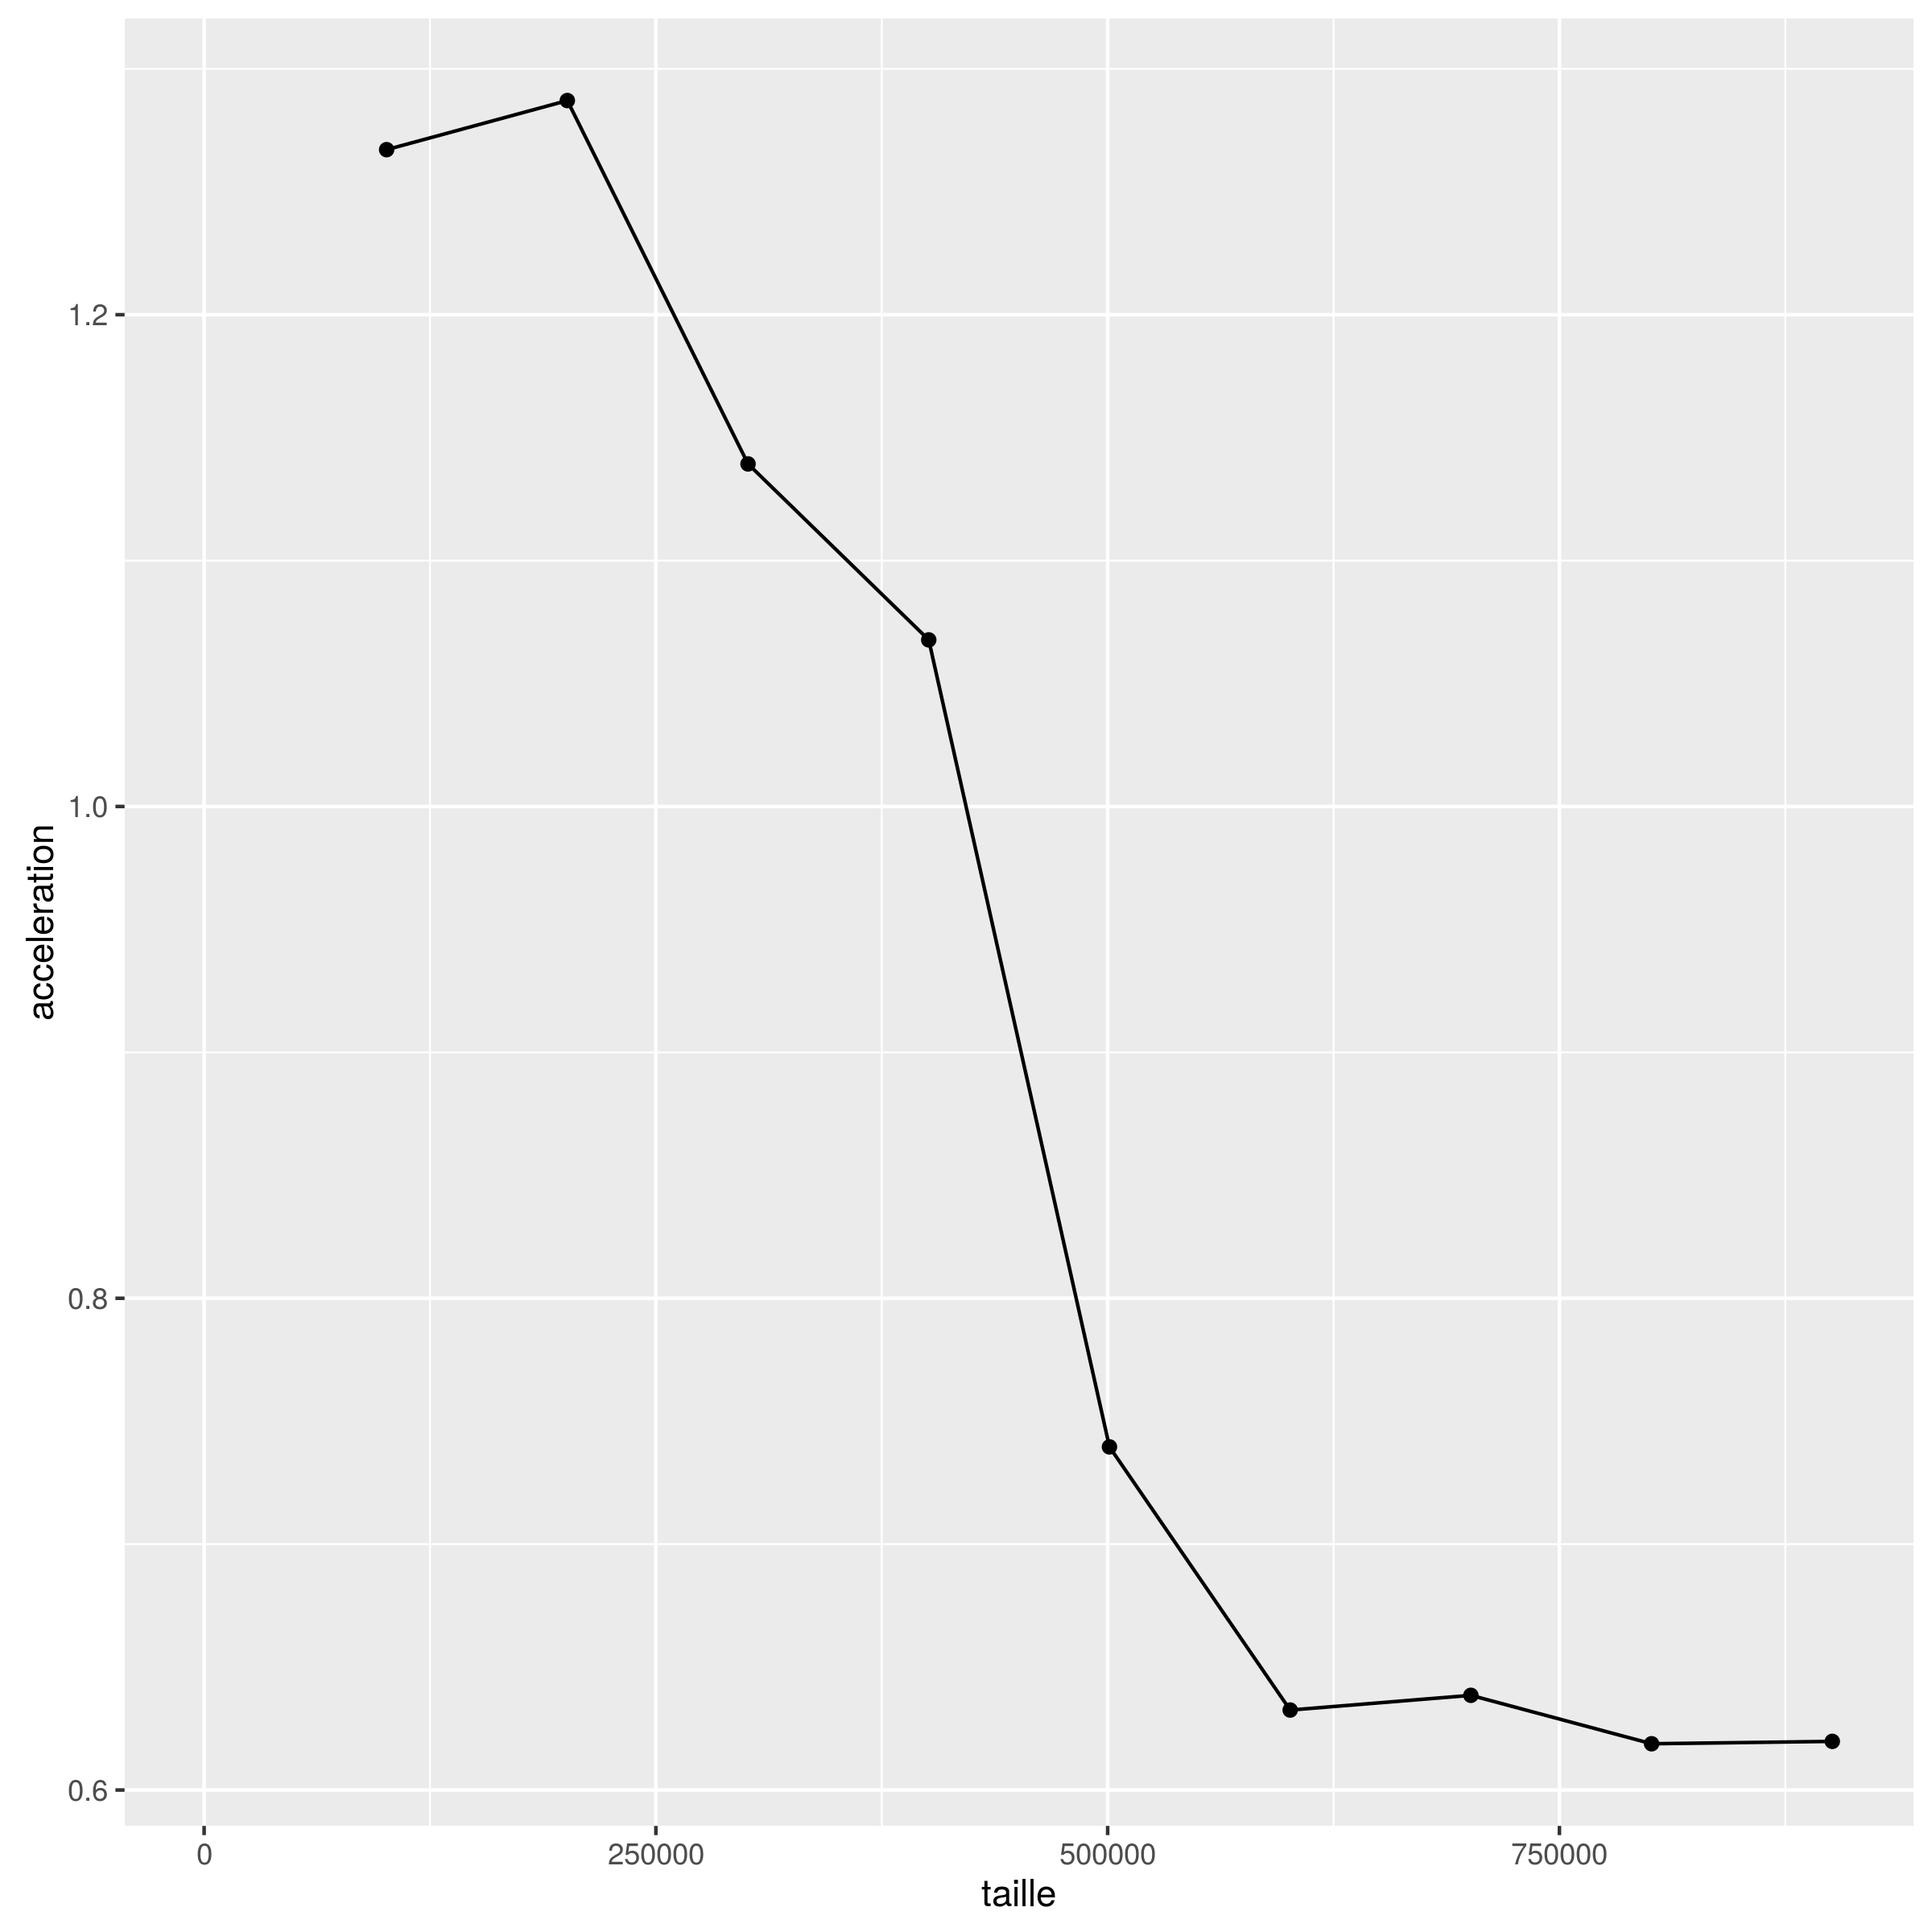
\includegraphics[scale=0.5] {graphes/temps_user_accel2.png}
\end{figure}
Nous observons que pour des vecteurs d'une taille inf\'erieur \`a 400000, l'acc\'el\'eration est sup\'erieur \`a 1. N\'eanmoins pass\'e ce seuil,  l'acc\'el\'eration est maintenant inf\'erieur \`a un, cela signifie que le temps CPU cumul\'e de l'utilisateur finit par \^{e}tre plus \'elev\'e avec 2 threads qu'en s\'equentiel. Cette acc\'el\'eration finit par tendre verss 0.6.


\section{Avec 3 threads}
\subsection{Temps d'ex\'ecution}

\begin{figure}[H] \center
   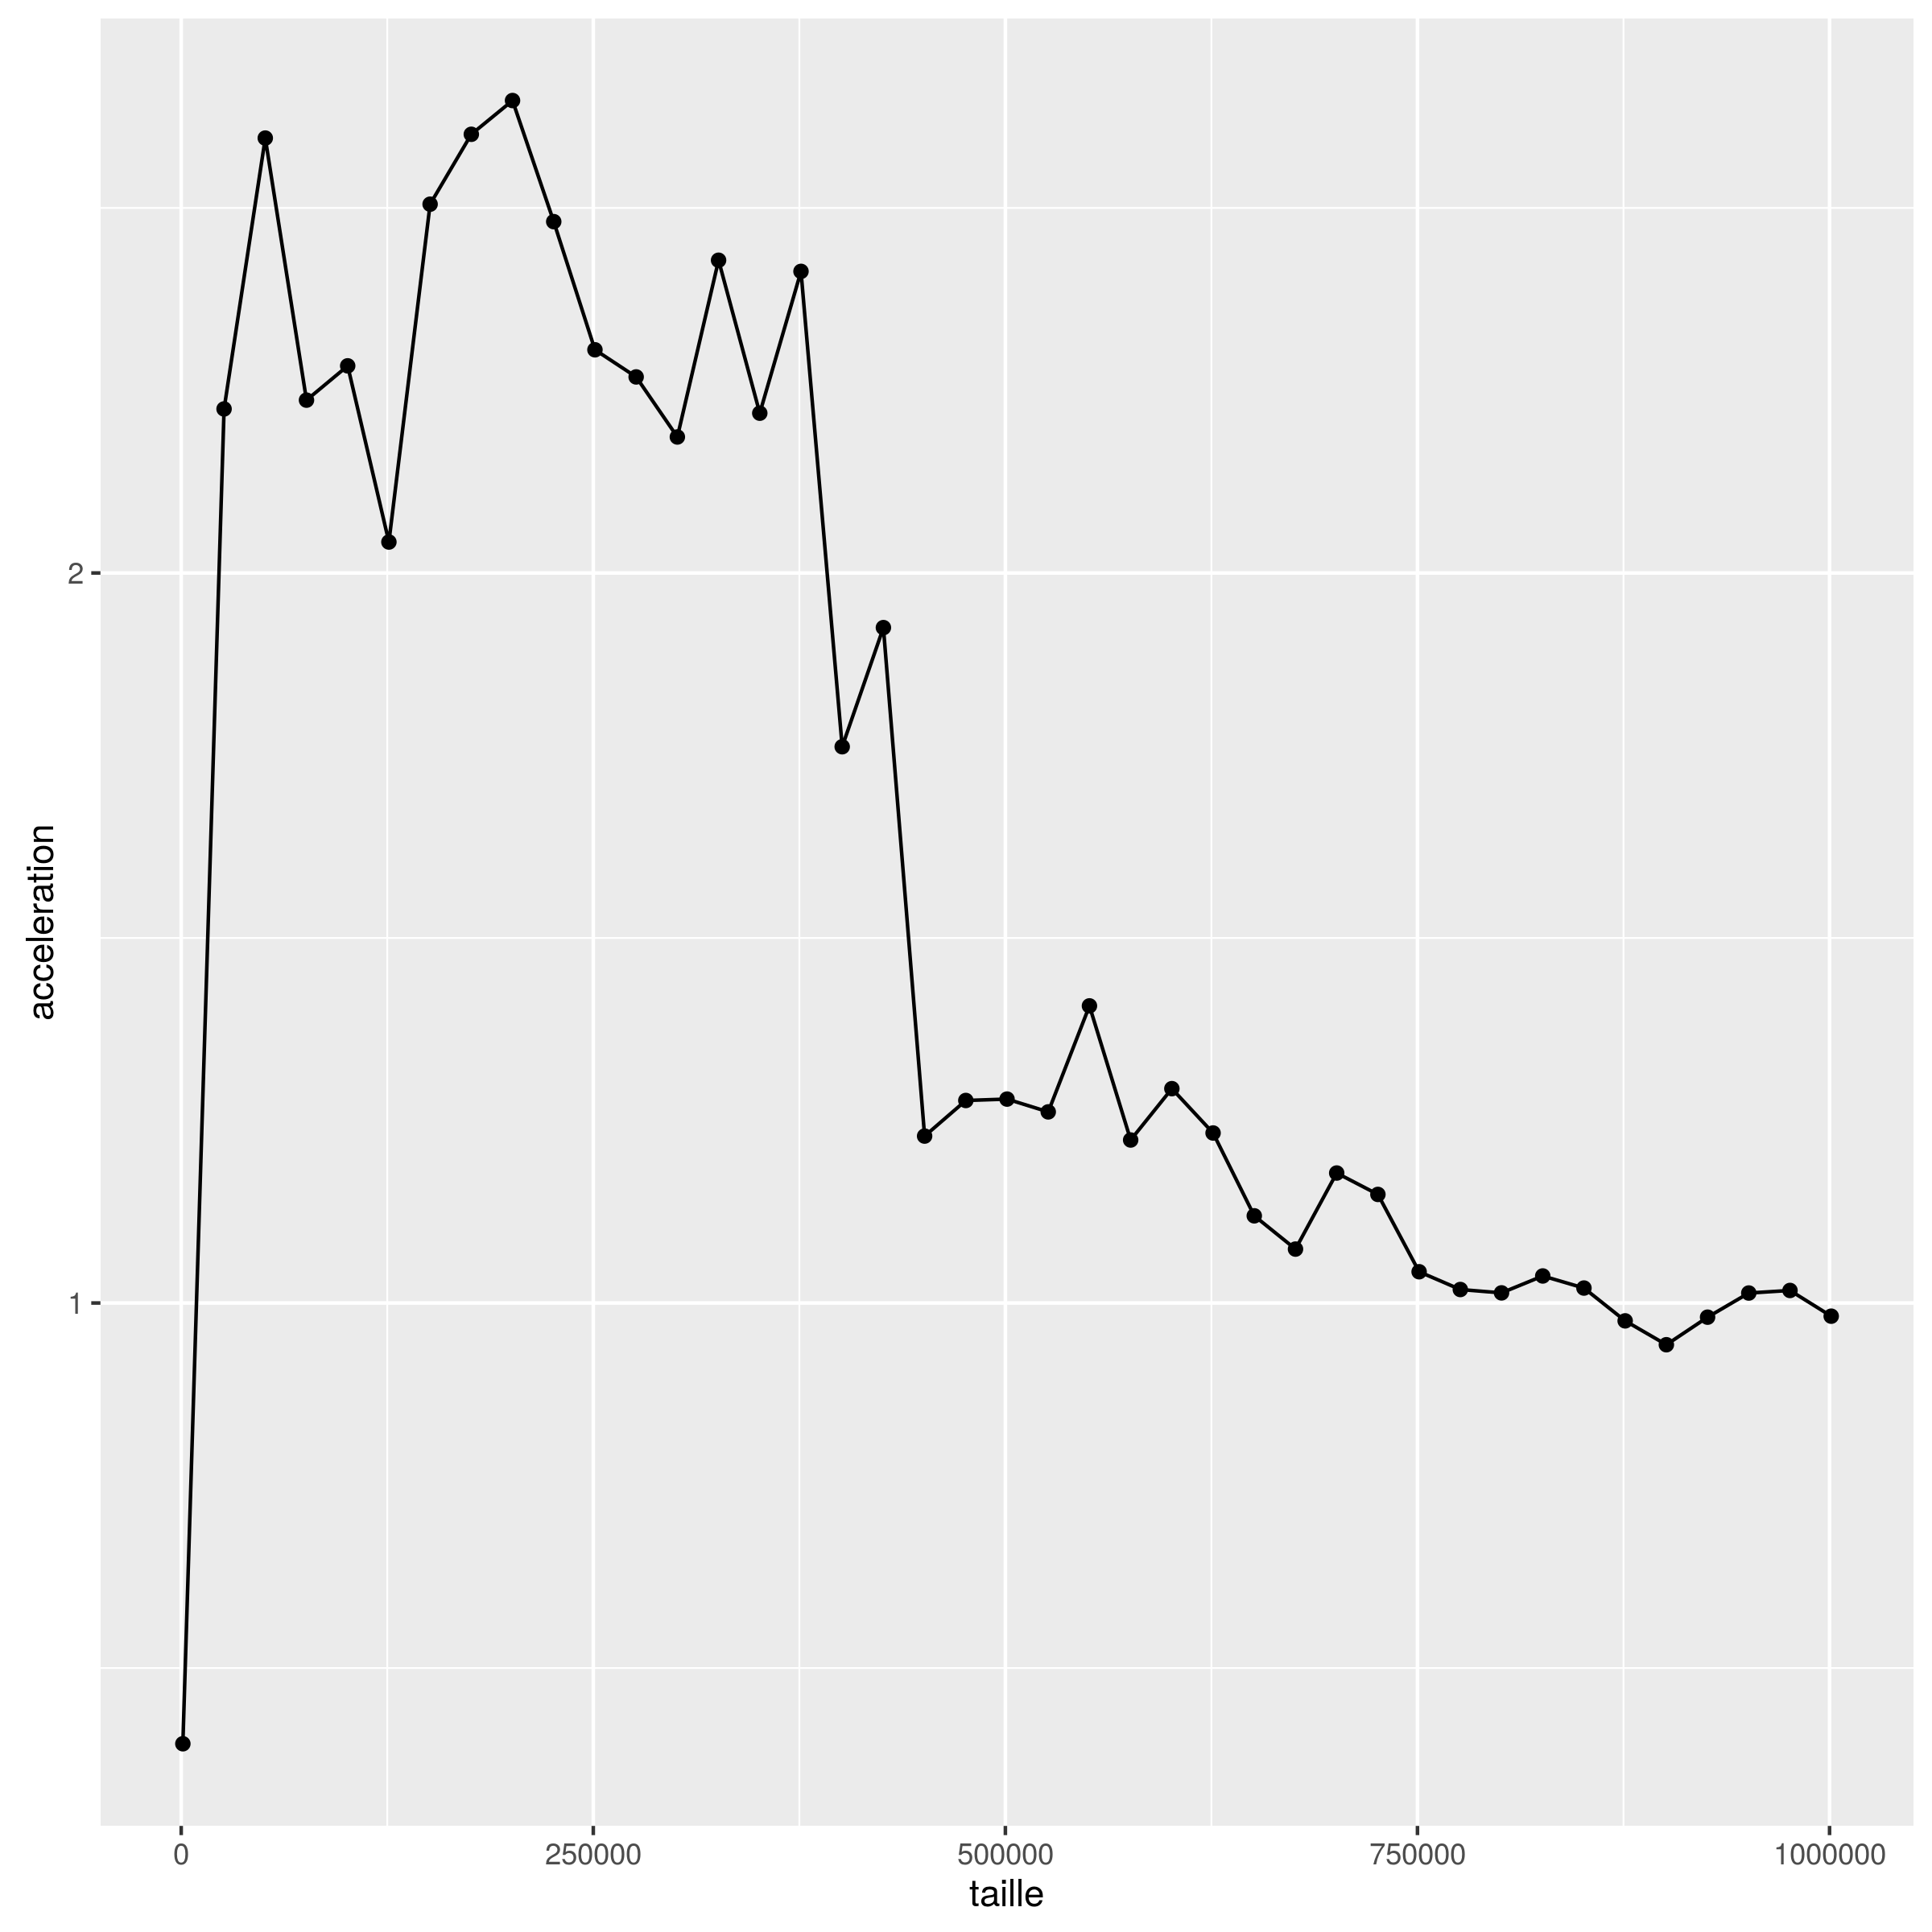
\includegraphics[scale=0.5] {graphes/global_temps_machine_accel3.png}
\end{figure}

Nous observons que pour des vecteurs allant d'une taille de 1000 \'el\'ements \`a 1000000 d'\'el\'ements, l'acc\'el\'eration est toujours sup\'erieur \`a 1. Nous observons aussi que l'acc\'el\'eration est la plus grande, pour des vecteurs d'une taille d'environ 200000 \'el\'ements. Pass\'e ce seuil, le niveau de l'acc\'el\'eration baisse et finit par tendre vers 1.5, pass\' le seuil des 700000 \'el\'ements.   


\subsection{Temps CPU cumul\'e de l'utilisateur}
\begin{figure}[H] \center
   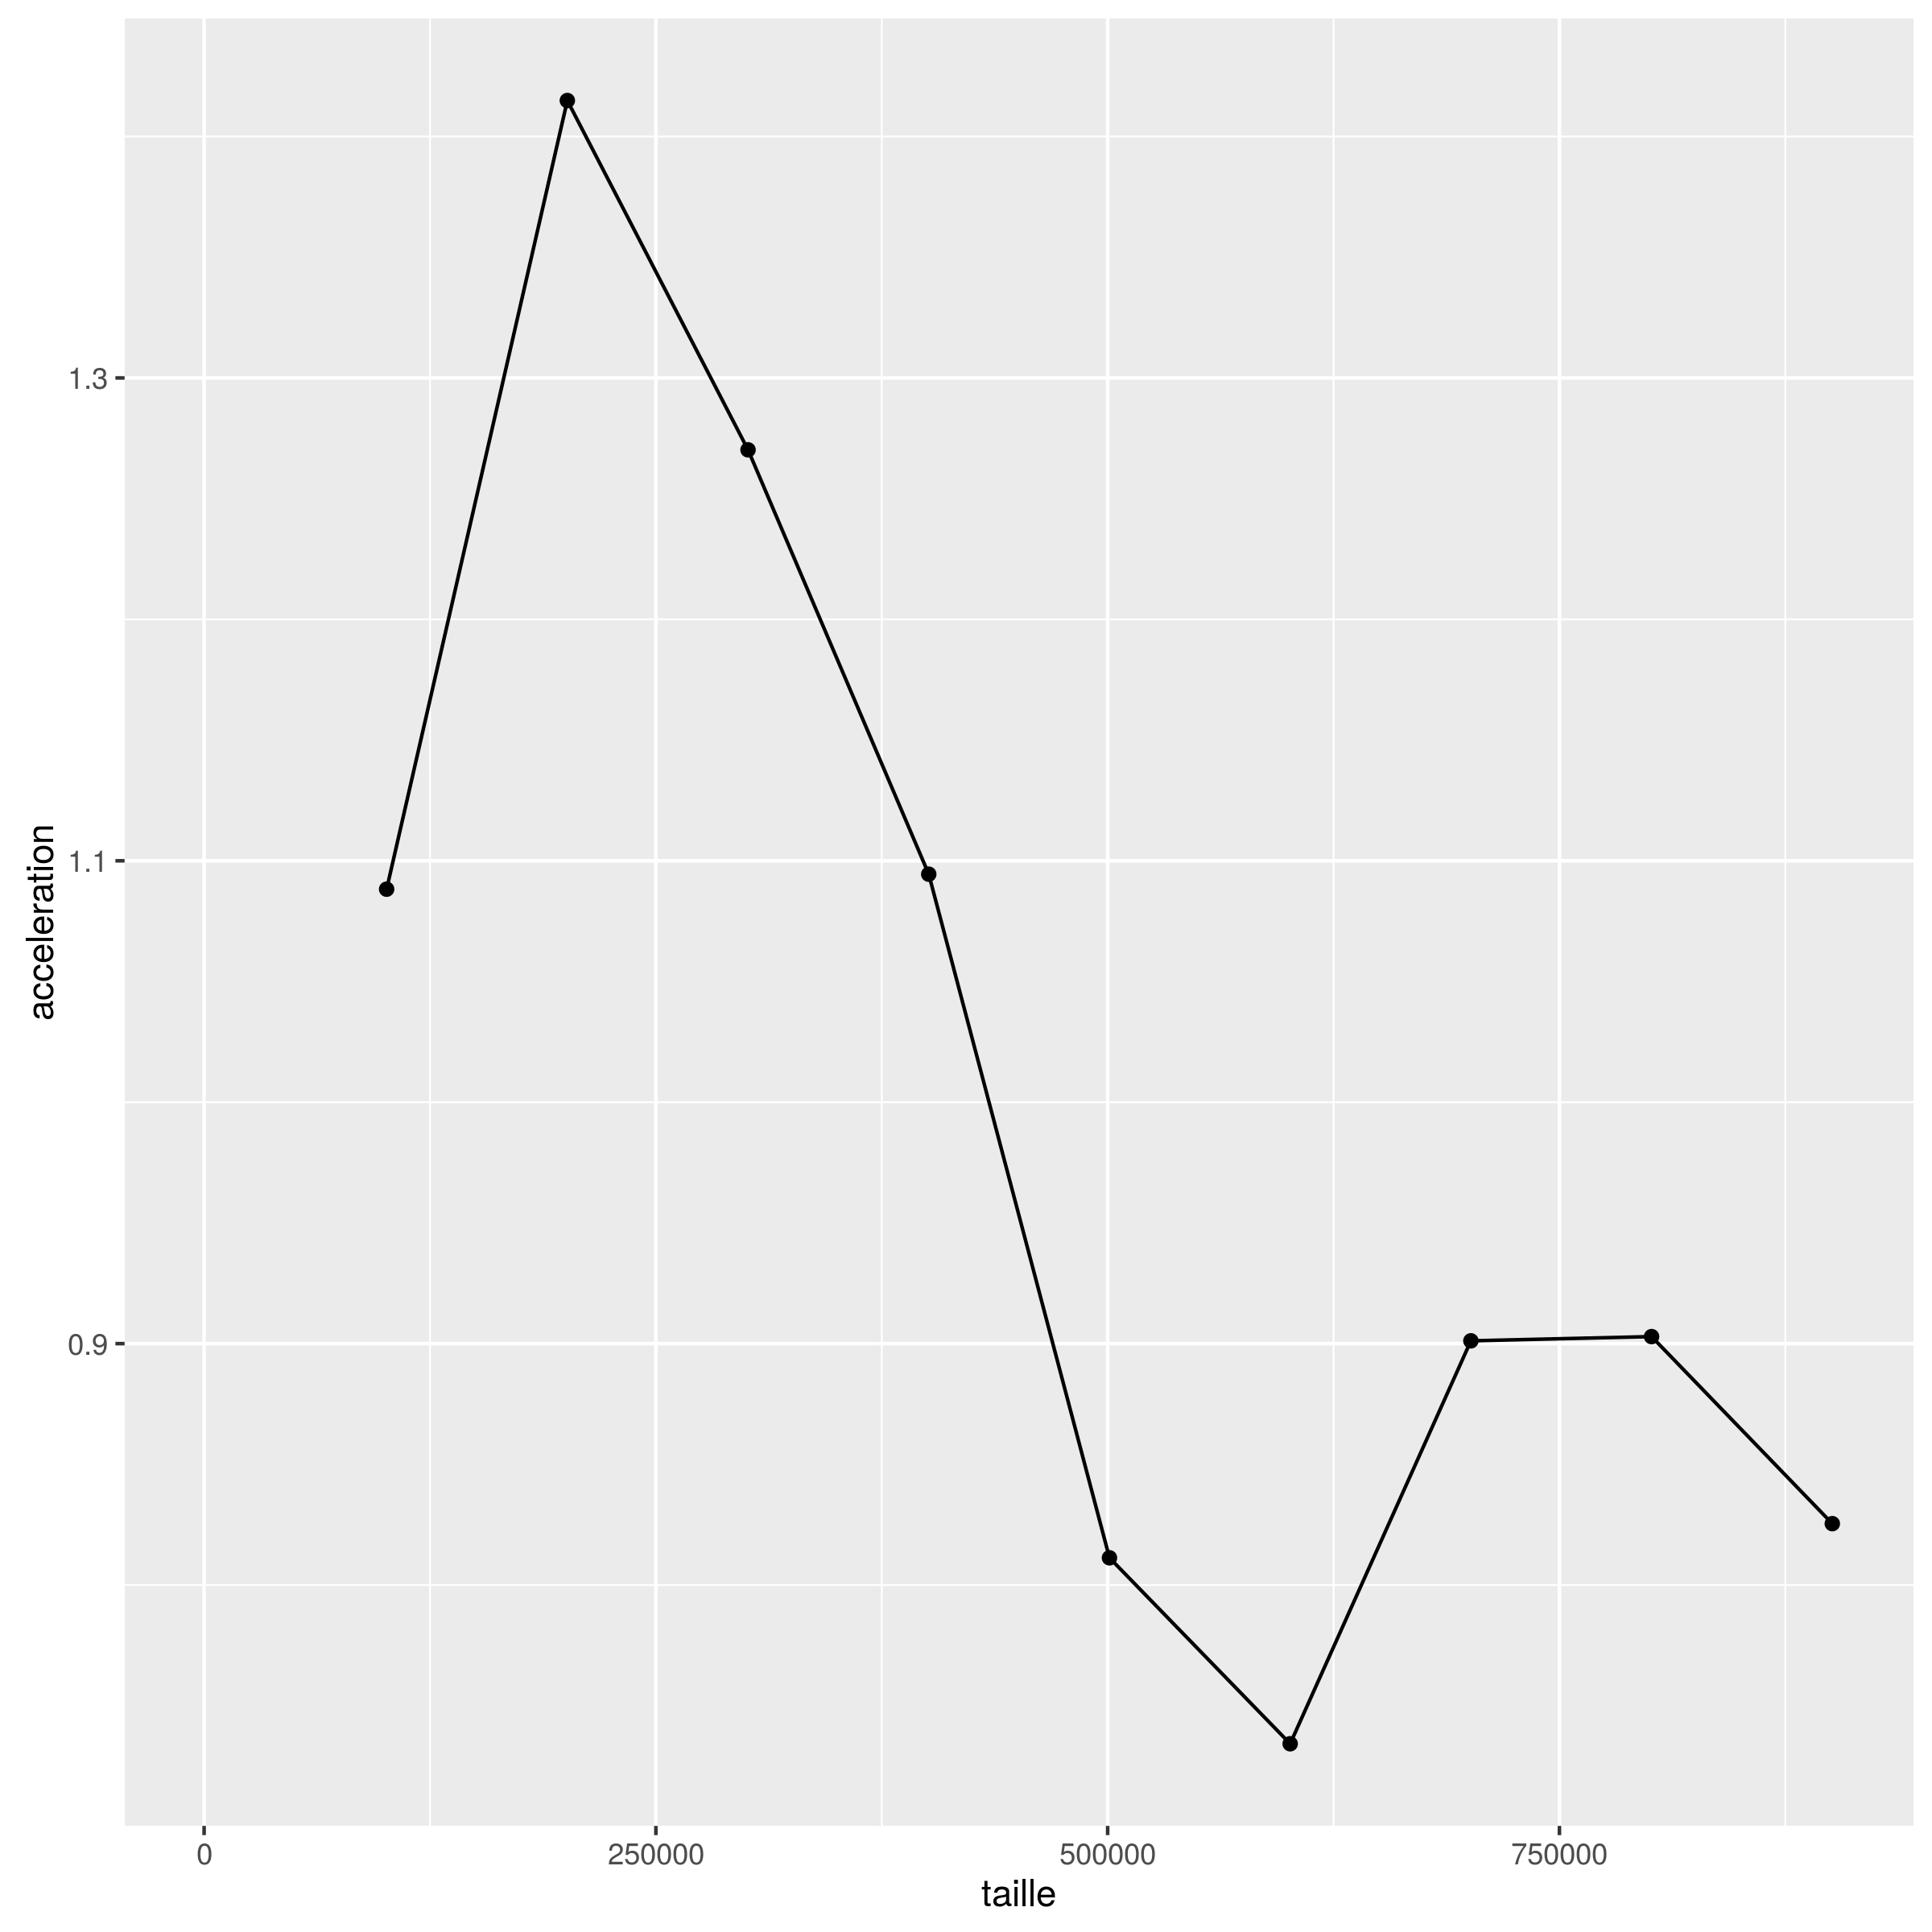
\includegraphics[scale=0.5] {graphes/temps_user_accel3.png}
\end{figure}
Nous observons que pour des vecteurs d'une taille inf\'erieur \`a 400000, l'acc\'el\'eration est sup\'erieur \`a 1. N\'eanmoins pass\'e ce seuil,  l'acc\'el\'eration est maintenant inf\'erieur \`a un, cela signifie que le temps CPU cumul\'e de l'utilisateur finit par \^{e}tre plus \'elev\'e avec 3 threads qu'en s\'equentiel. Cette acc\'el\'eration finit par tendre verss 0.7.


\section{Avec 4 threads}
\subsection{Temps d'ex\'ecution}

\begin{figure}[H] \center
   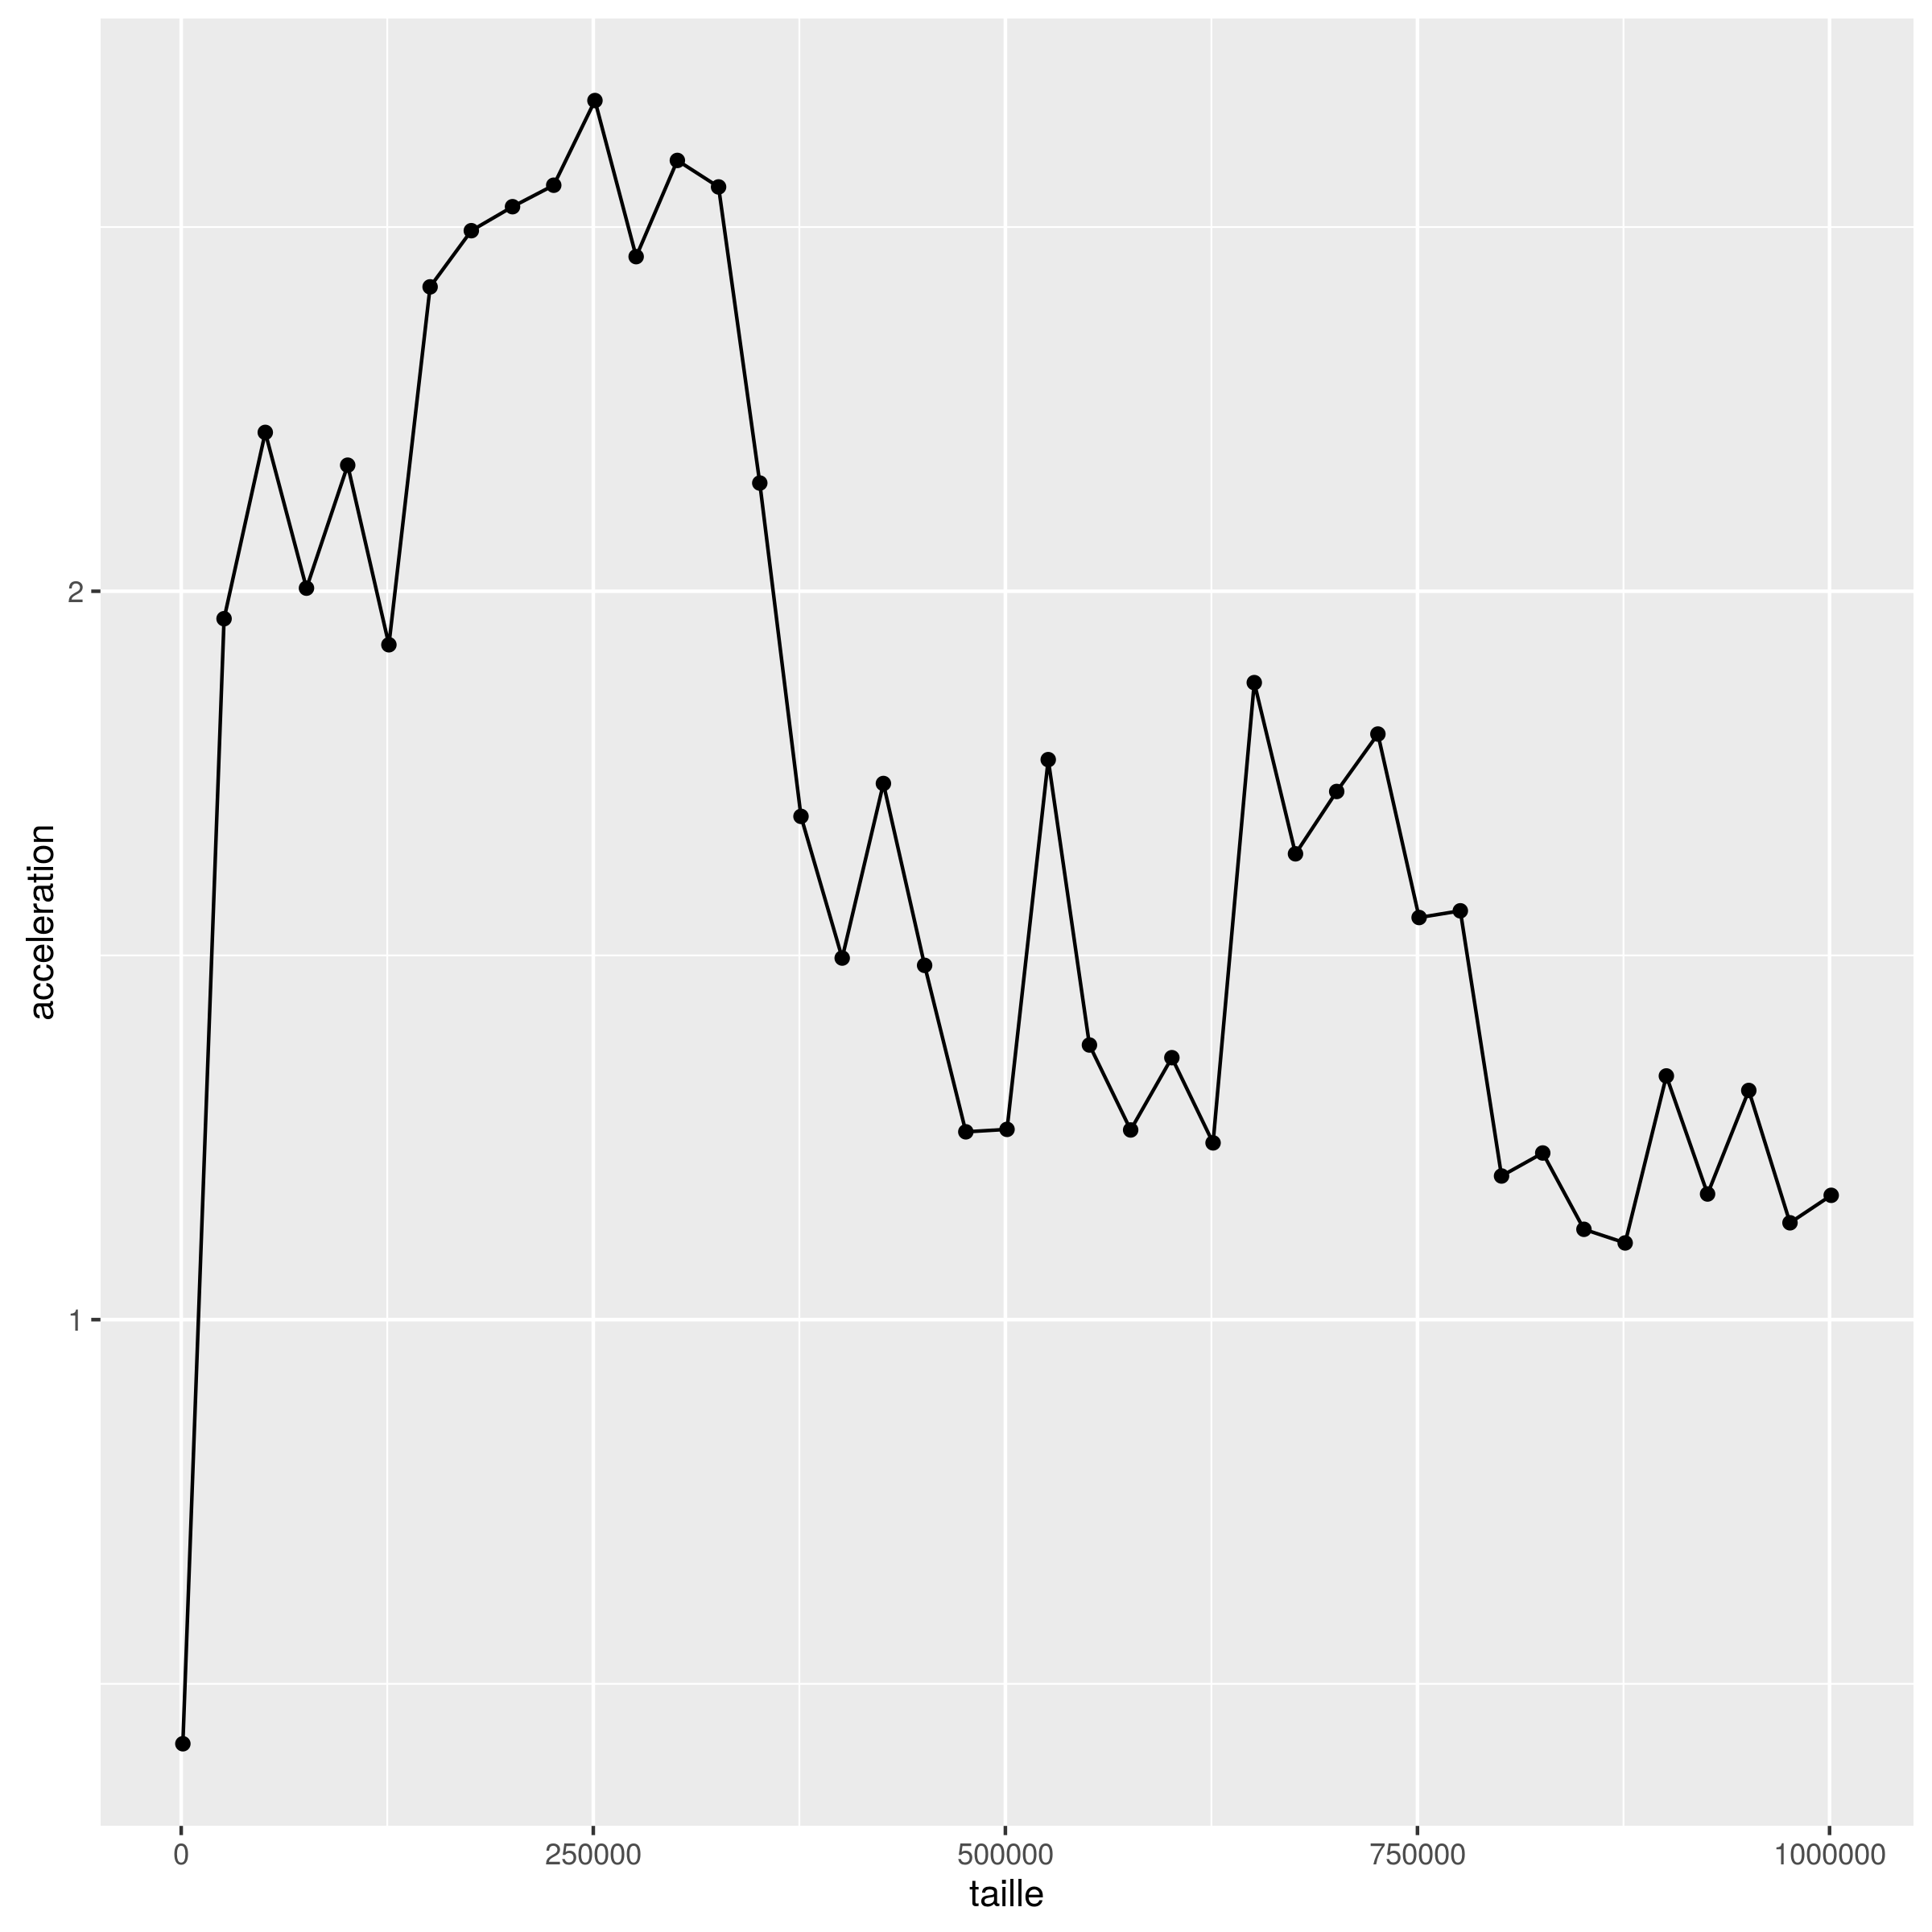
\includegraphics[scale=0.5] {graphes/global_temps_machine_accel4.png}
\end{figure}

Nous observons que pour des vecteurs allant d'une taille de 1000 \'el\'ements \`a 1000000 d'\'el\'ements, l'acc\'el\'eration est toujours sup\'erieur \`a 1. Nous observons aussi que l'acc\'el\'eration est la plus grande, pour des vecteurs d'une taille d'environ 200000 \'el\'ements. Pass\'e ce seuil, le niveau de l'acc\'el\'eration baisse (et finit par tendre vers un, pass\' le seuil des 700000 \'el\'ements).   


\subsection{Temps CPU cumul\'e de l'utilisateur}
\begin{figure}[H] \center
   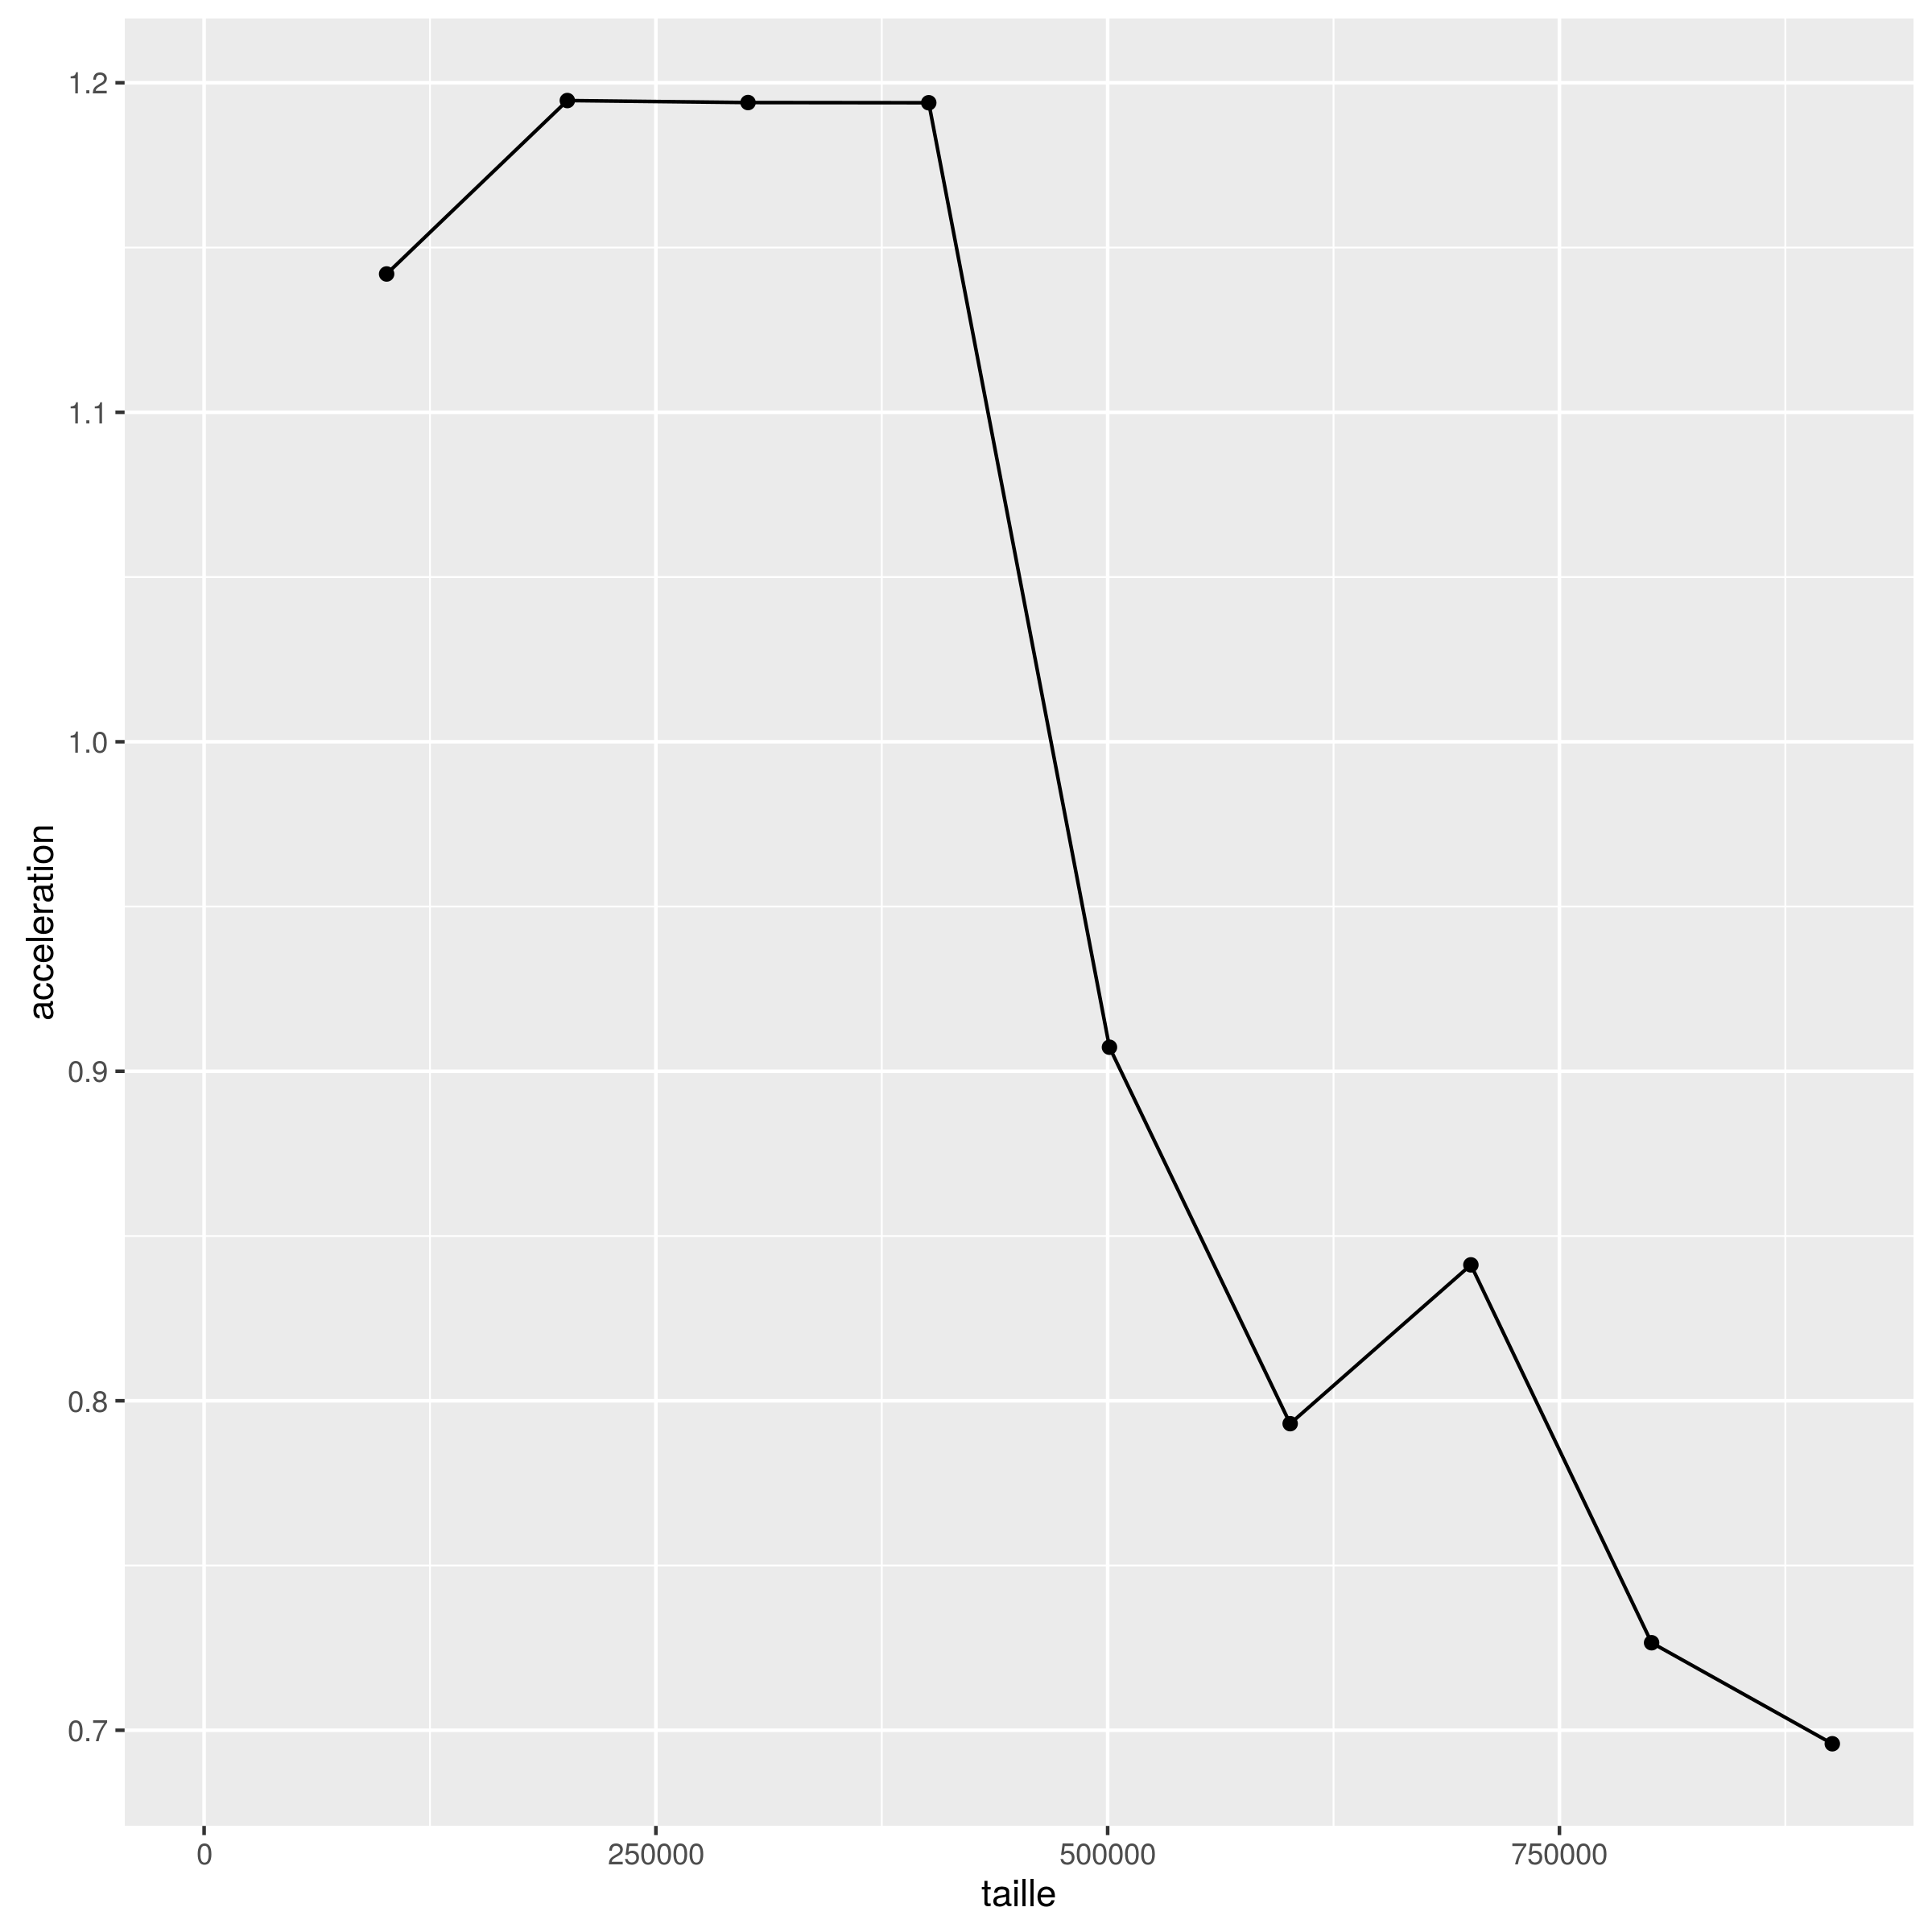
\includegraphics[scale=0.5] {graphes/temps_user_accel4.png}
\end{figure}
Nous observons que pour des vecteurs d'une taille inf\'erieur \`a 500000, l'acc\'el\'eration est sup\'erieur \`a 1. N\'eanmoins pass\'e ce seuil,  l'acc\'el\'eration est maintenant inf\'erieur \`a un, cela signifie que le temps CPU cumul\'e de l'utilisateur finit par \^{e}tre plus \'elev\'e avec 4 threads qu'en s\'equentiel. Cette acc\'el\'eration finit par tendre verss 0.7.


\section{Avec 5 threads}
\subsection{Temps d'ex\'ecution}

\begin{figure}[H] \center
   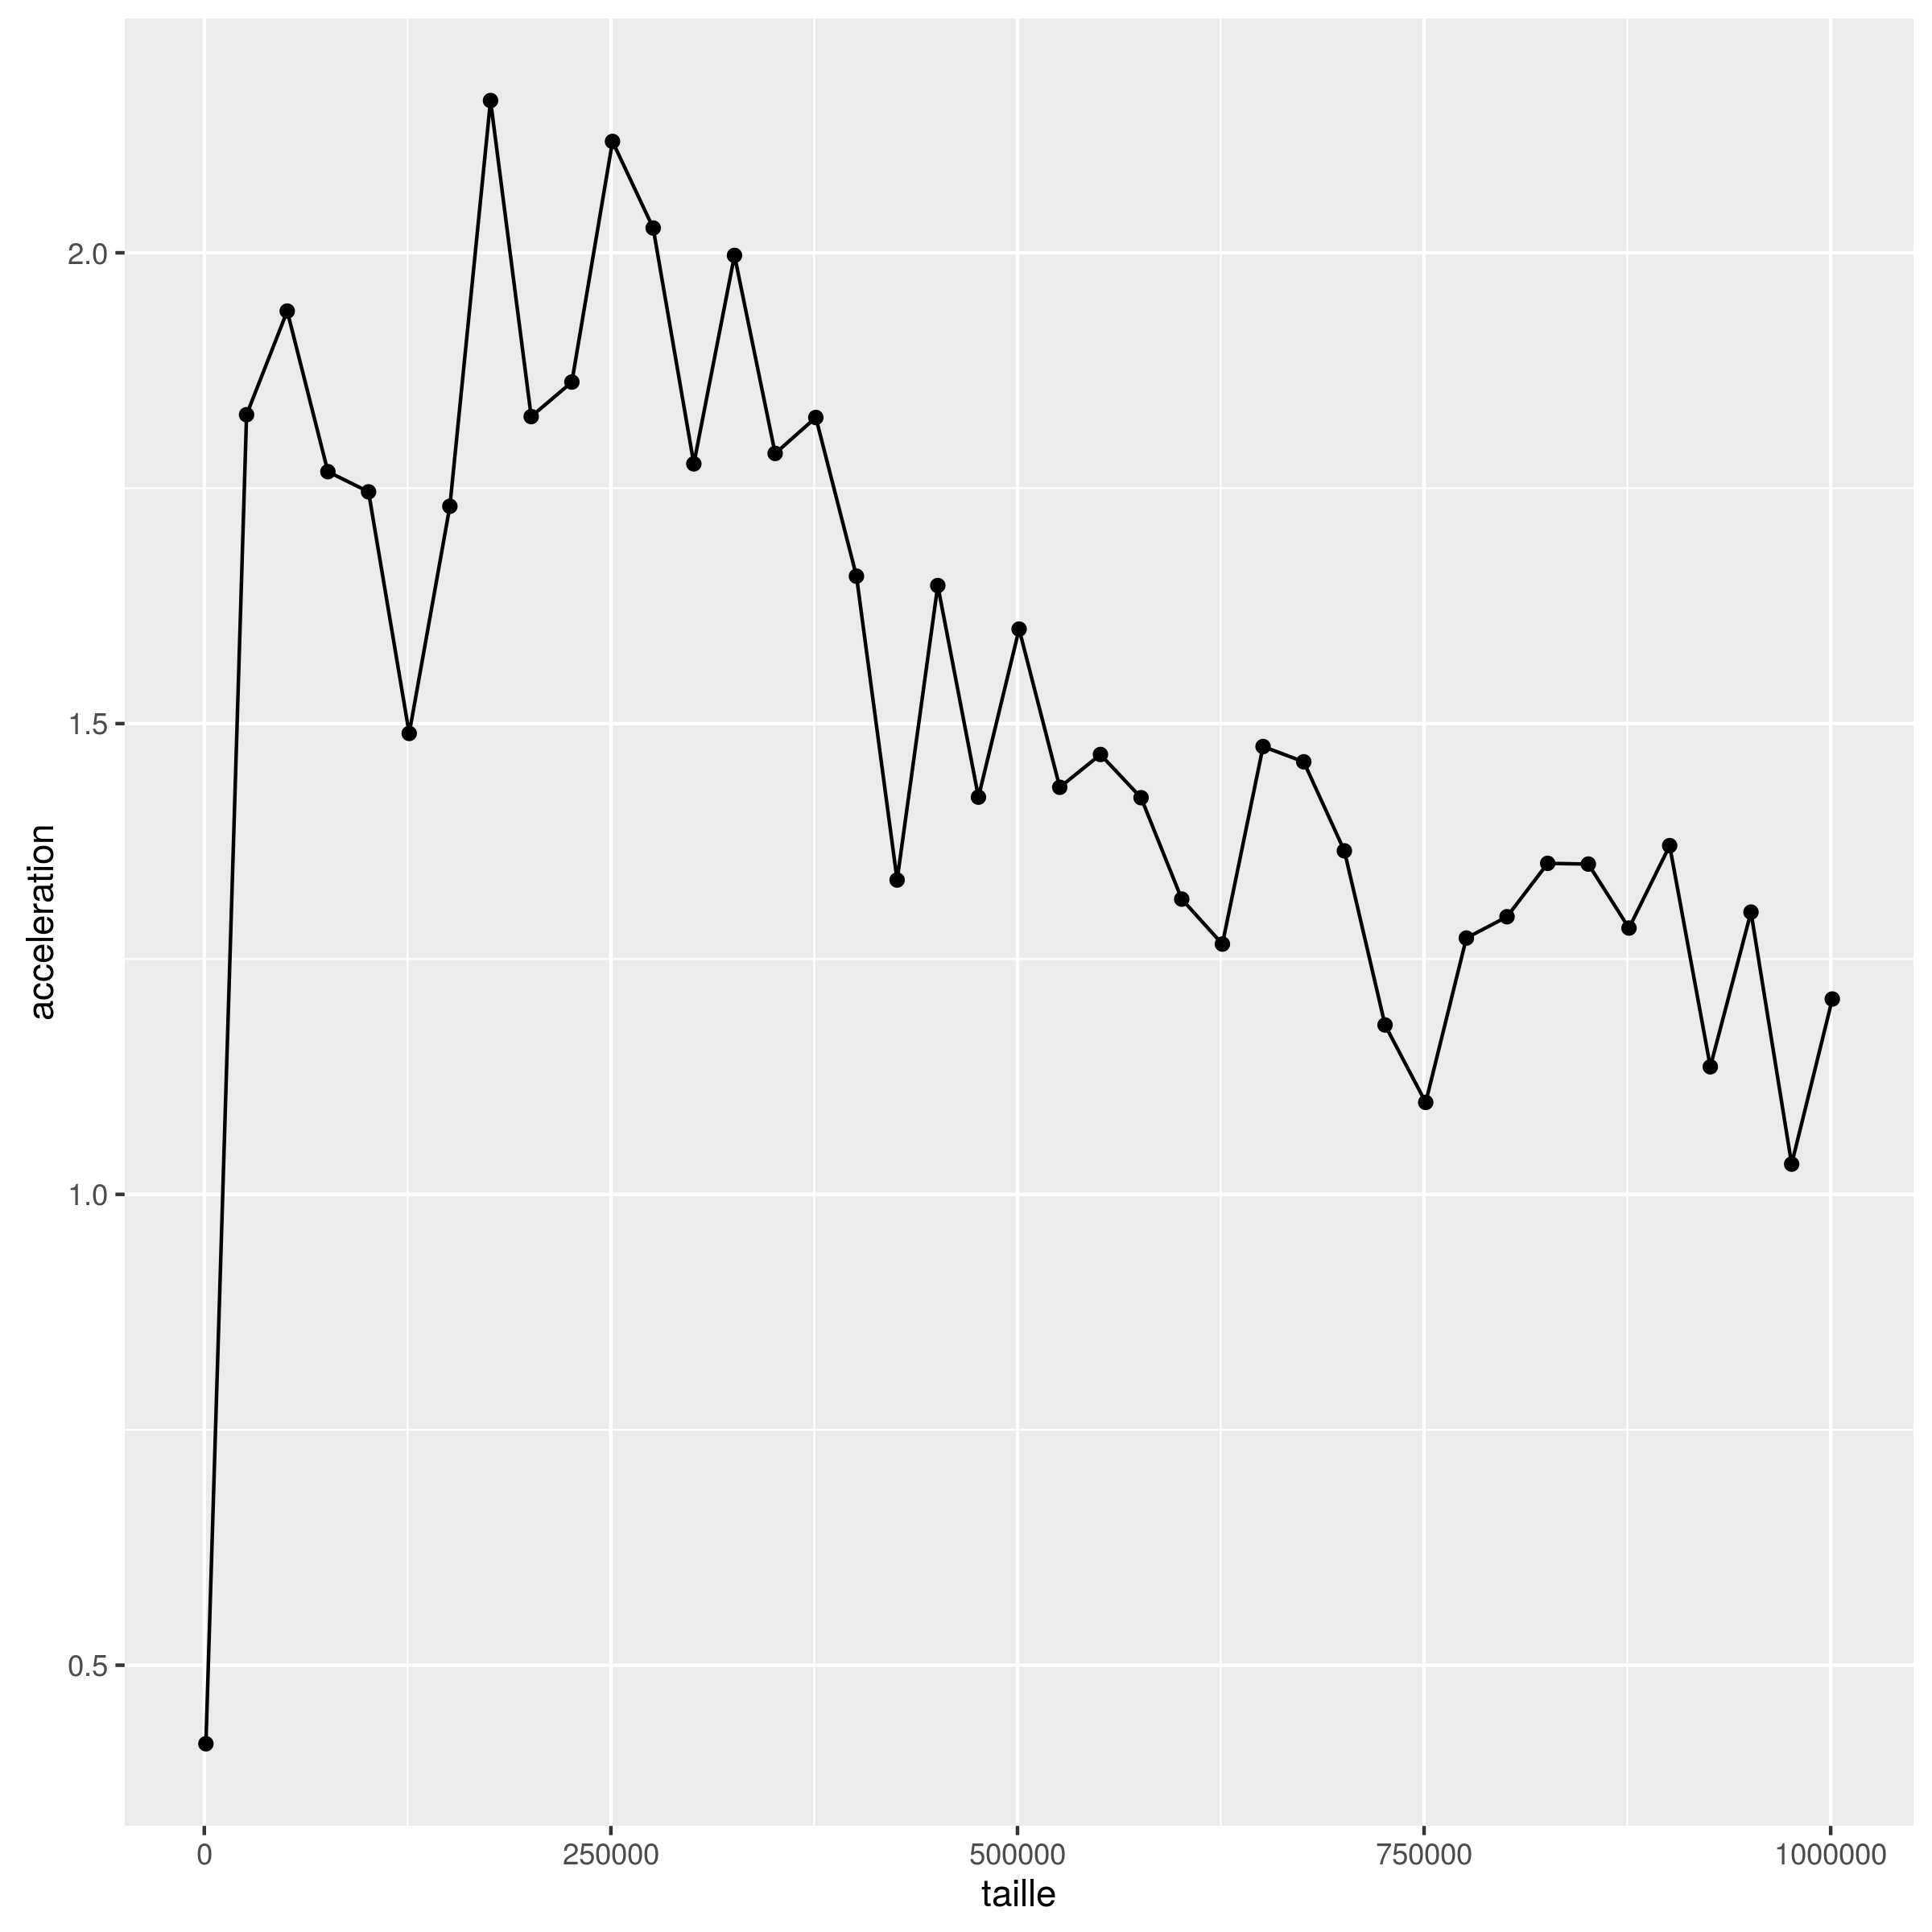
\includegraphics[scale=0.5] {graphes/global_temps_machine_accel5.png}
\end{figure}

Nous observons que pour des vecteurs allant d'une taille de 1000 \'el\'ements \`a 1000000 d'\'el\'ements, l'acc\'el\'eration est toujours sup\'erieur \`a 1. Nous observons aussi que l'acc\'el\'eration est la plus grande, pour des vecteurs d'une taille d'environ 200000 \'el\'ements. Pass\'e ce seuil, le niveau de l'acc\'el\'eration baisse et finit par tendre vers 1.3, pass\' le seuil des 800000 \'el\'ements.   


\subsection{Temps CPU cumul\'e de l'utilisateur}
\begin{figure}[H] \center
   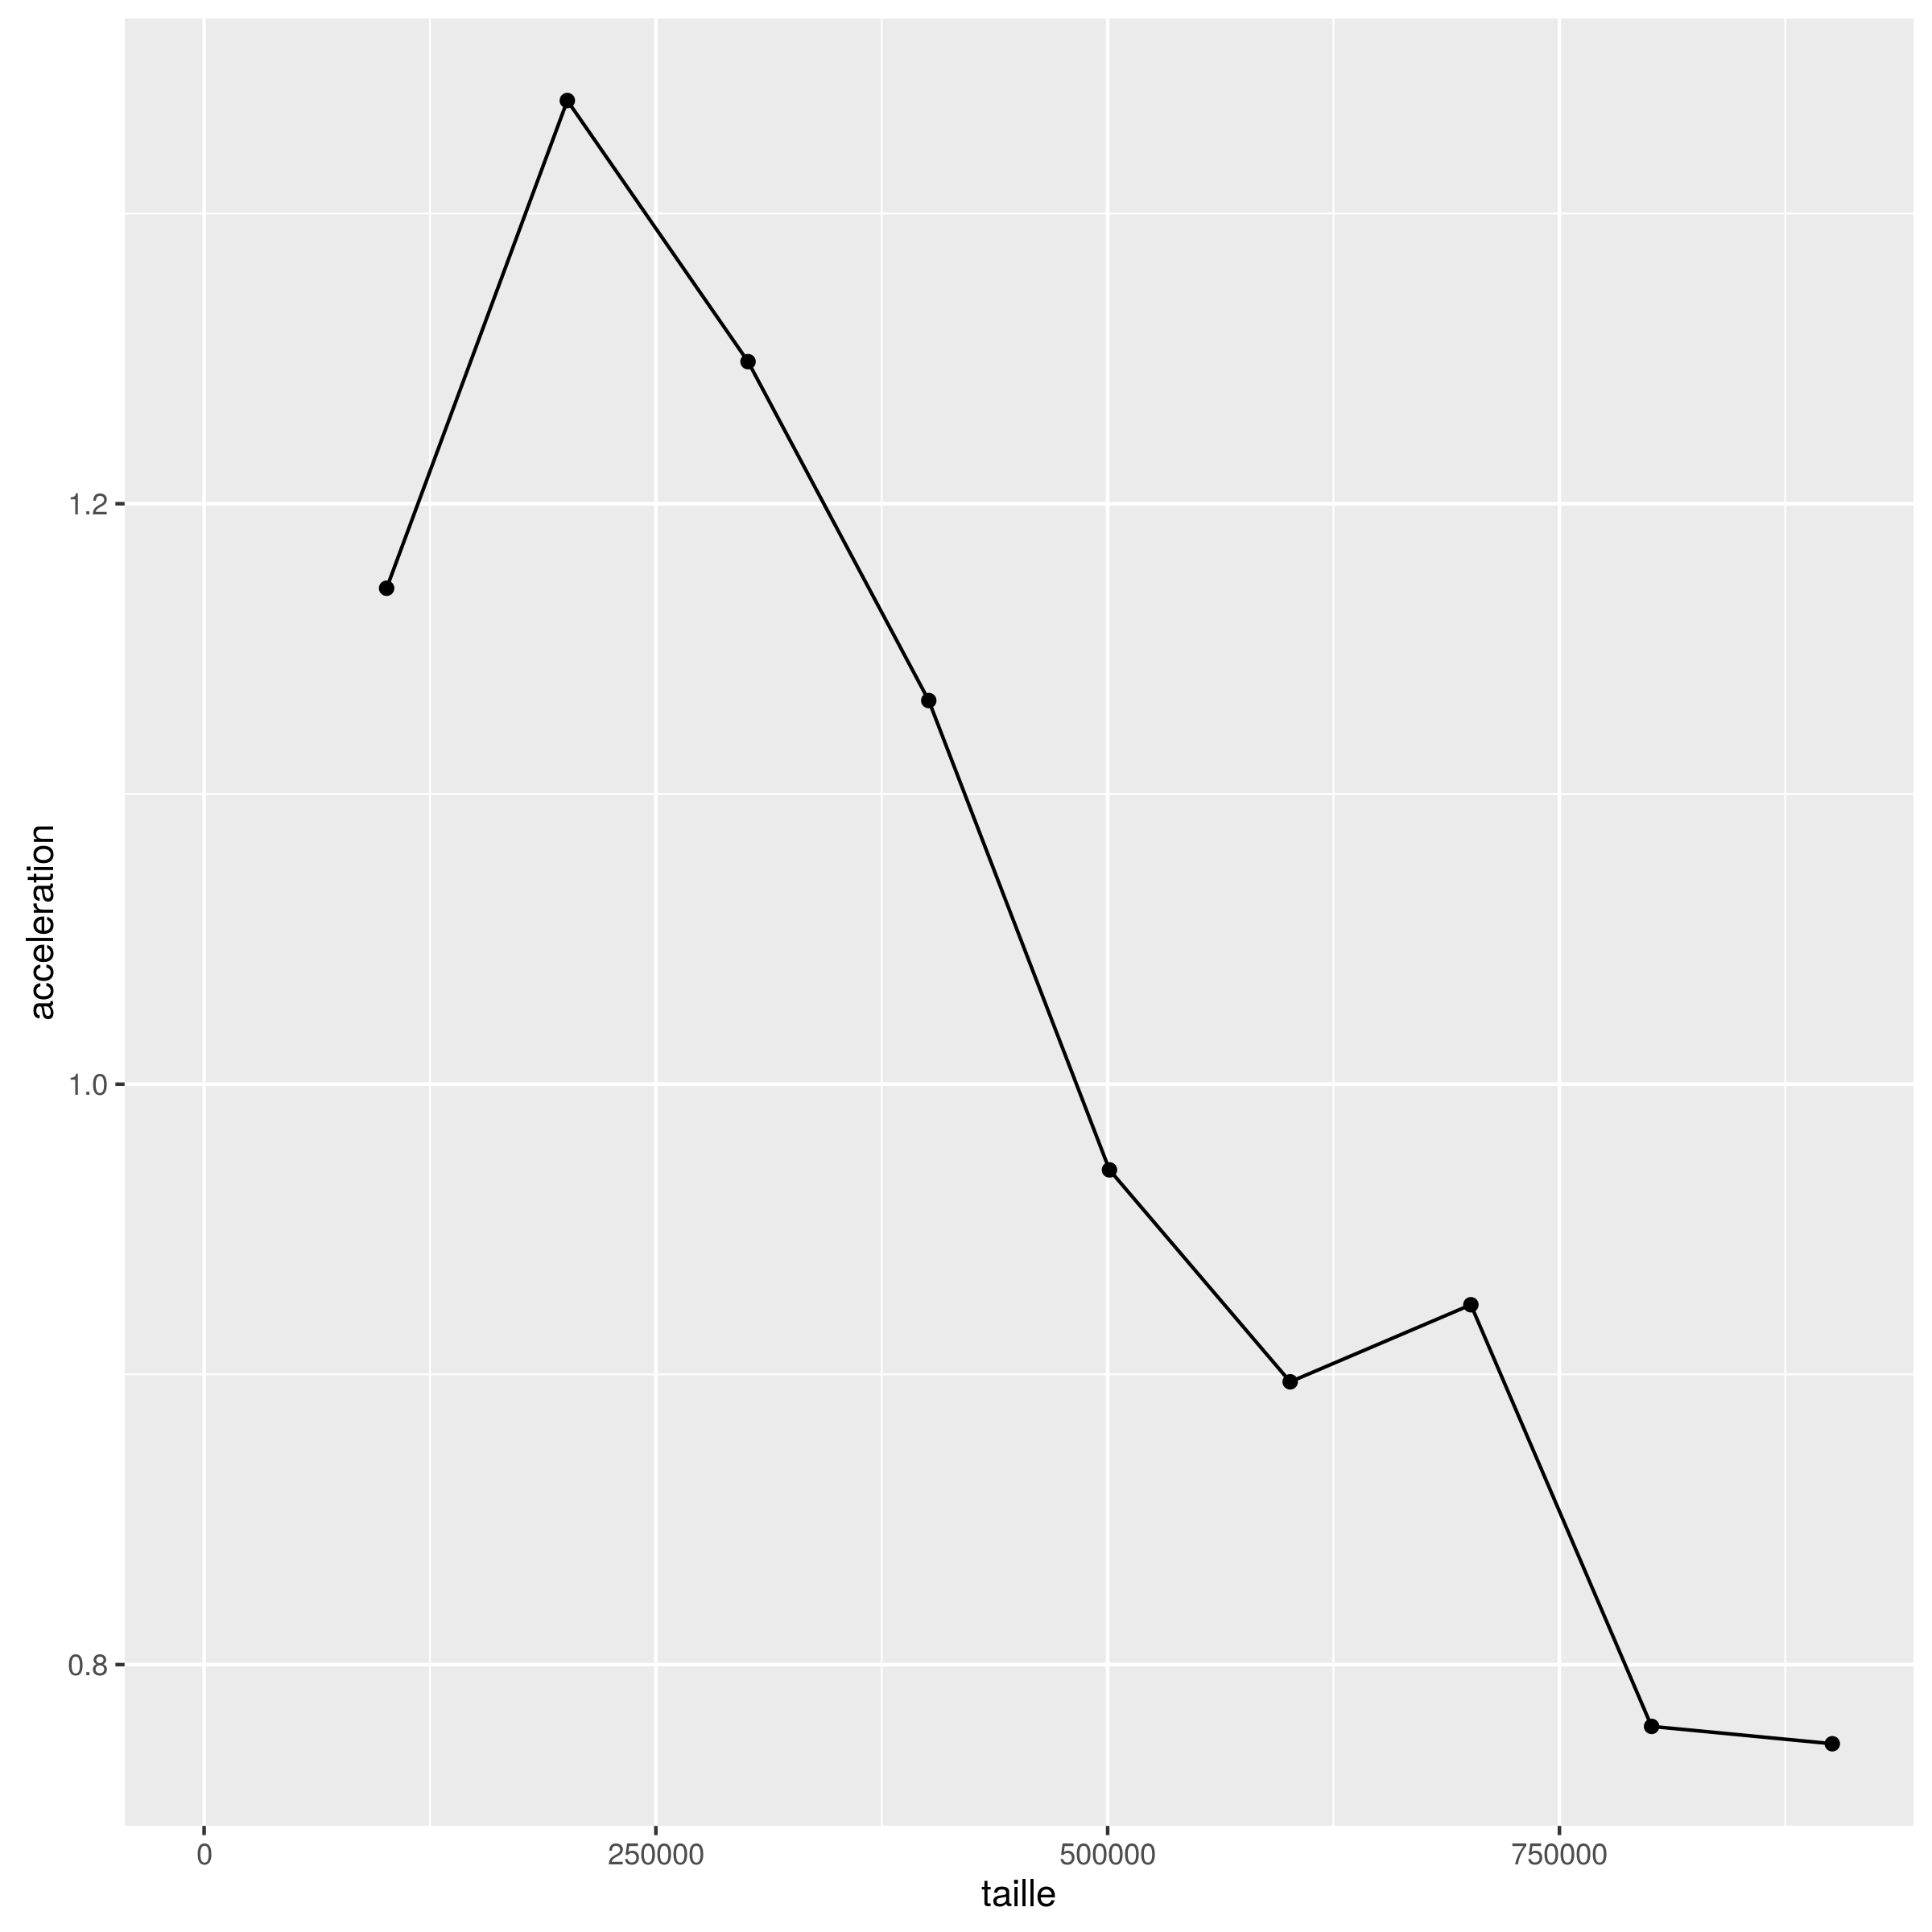
\includegraphics[scale=0.5] {graphes/temps_user_accel5.png}
\end{figure}
Nous observons que pour des vecteurs d'une taille inf\'erieur \`a 450000, l'acc\'el\'eration est sup\'erieur \`a 1. N\'eanmoins pass\'e ce seuil,  l'acc\'el\'eration est maintenant inf\'erieur \`a un, cela signifie que le temps CPU cumul\'e de l'utilisateur finit par \^{e}tre plus \'elev\'e avec 5 threads qu'en s\'equentiel. Cette acc\'el\'eration finit par tendre verss 0.7.


\section{Avec 6 threads}
\subsection{Temps d'ex\'ecution}

\begin{figure}[H] \center
   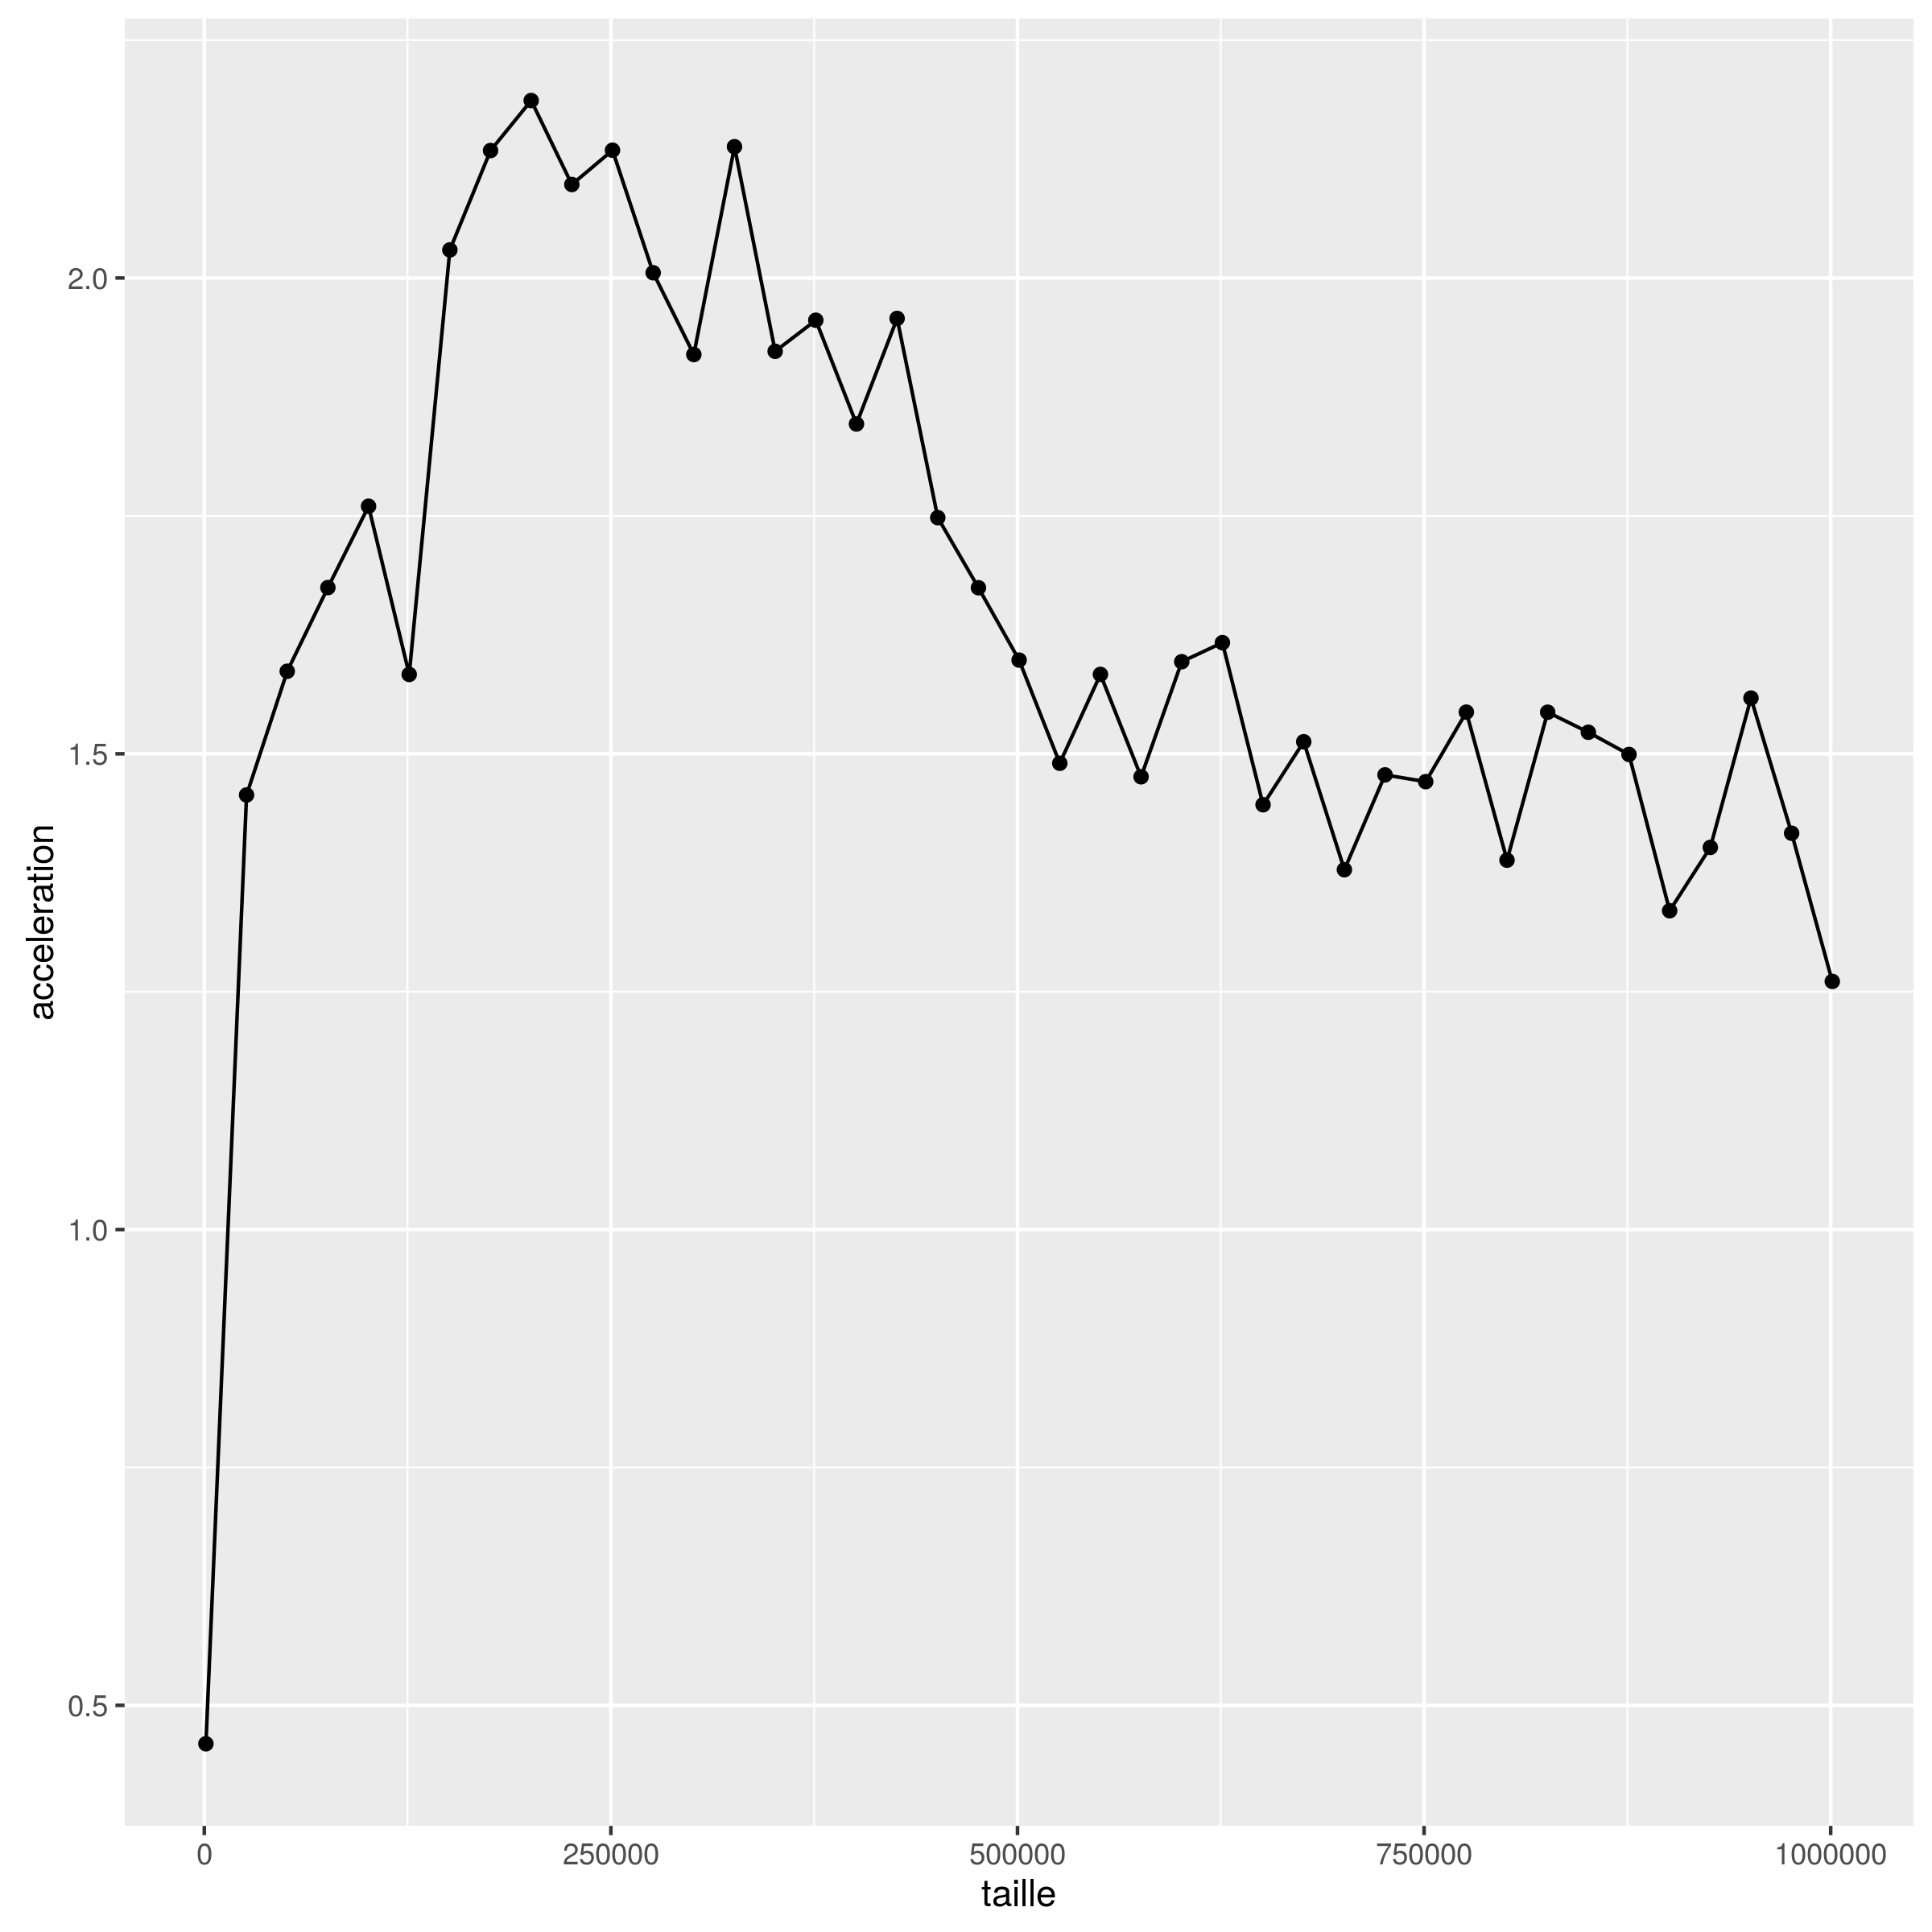
\includegraphics[scale=0.5] {graphes/global_temps_machine_accel6.png}
\end{figure}

Nous observons que pour des vecteurs allant d'une taille de 1000 \'el\'ements \`a 1000000 d'\'el\'ements, l'acc\'el\'eration est toujours sup\'erieur \`a 1. Nous observons aussi que l'acc\'el\'eration est la plus grande, pour des vecteurs d'une taille d'environ 200000 \'el\'ements. Pass\'e ce seuil, le niveau de l'acc\'el\'eration baisse et finit par tendre vers 1.5, pass\' le seuil des 500000 \'el\'ements.   


\subsection{Temps CPU cumul\'e de l'utilisateur}
\begin{figure}[H] \center
   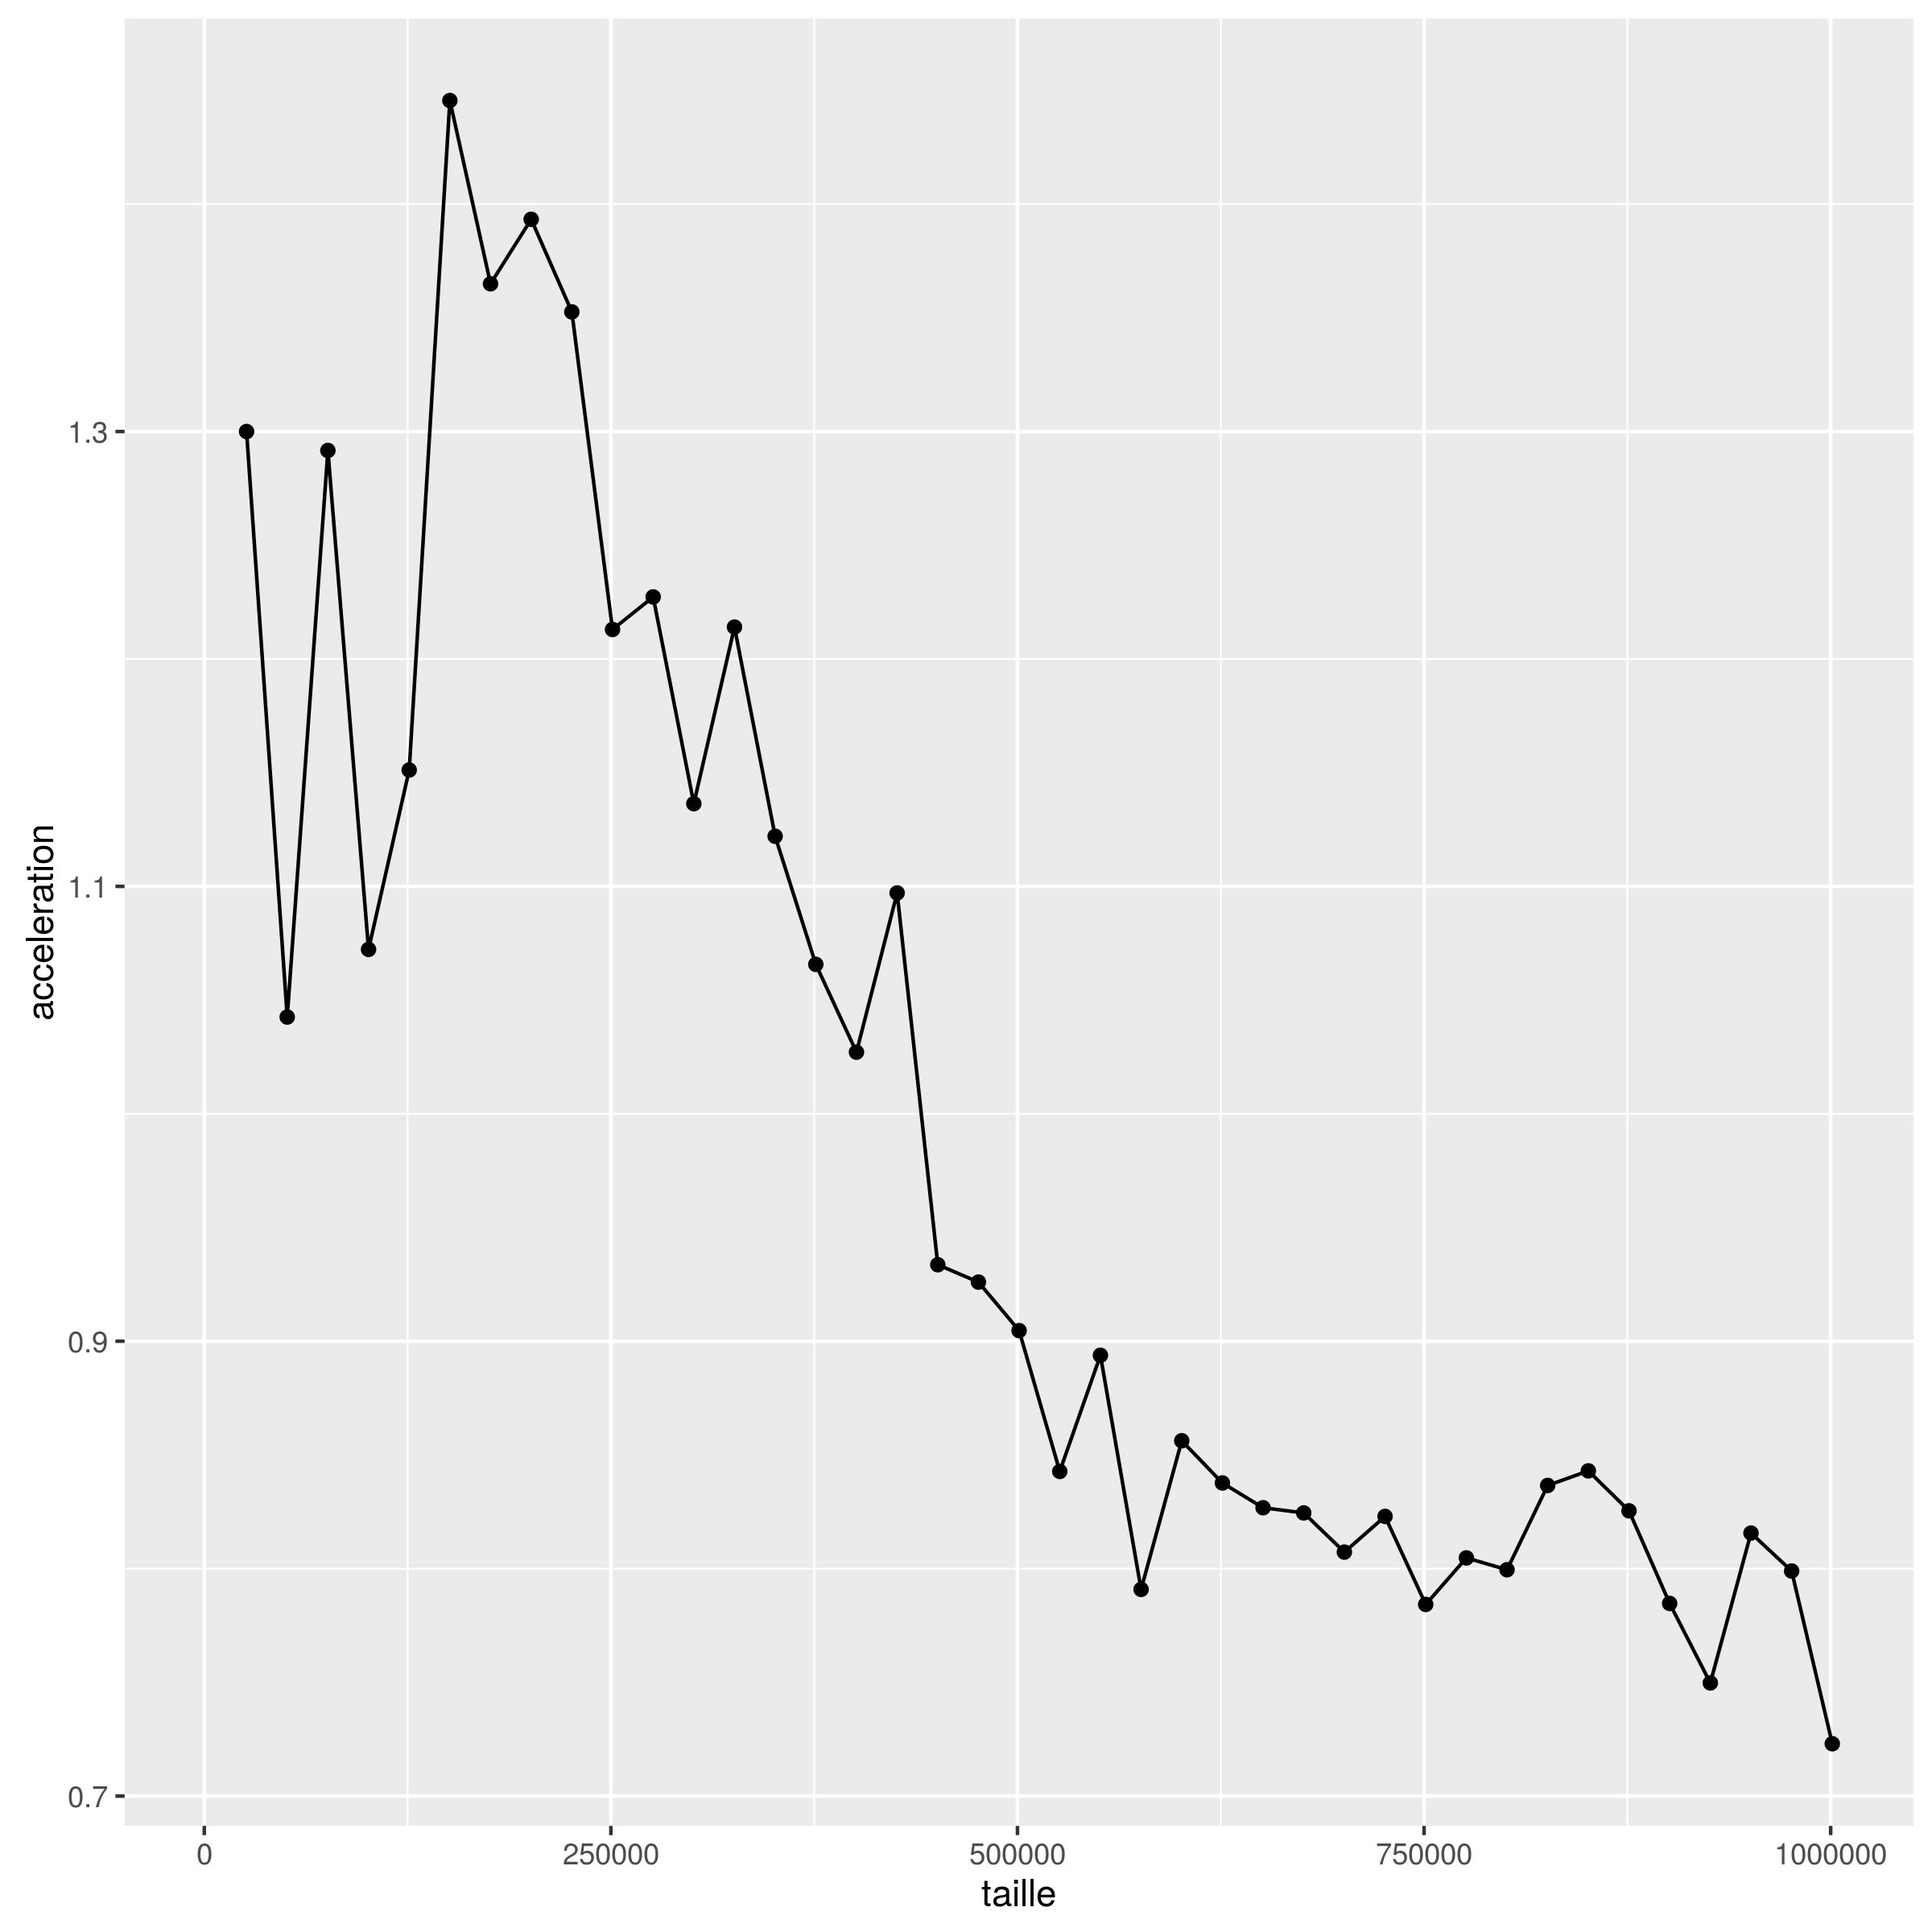
\includegraphics[scale=0.5] {graphes/temps_user_accel6.png}
\end{figure}
Nous observons que pour des vecteurs d'une taille inf\'erieur \`a 400000, l'acc\'el\'eration est sup\'erieur \`a 1. N\'eanmoins pass\'e ce seuil,  l'acc\'el\'eration est maintenant inf\'erieur \`a un, cela signifie que le temps CPU cumul\'e de l'utilisateur finit par \^{e}tre plus \'elev\'e avec 6 threads qu'en s\'equentiel. Cette acc\'el\'eration finit par tendre verss 0.9.


\section{Avec 7 threads}
\subsection{Temps d'ex\'ecution}

\begin{figure}[H] \center
   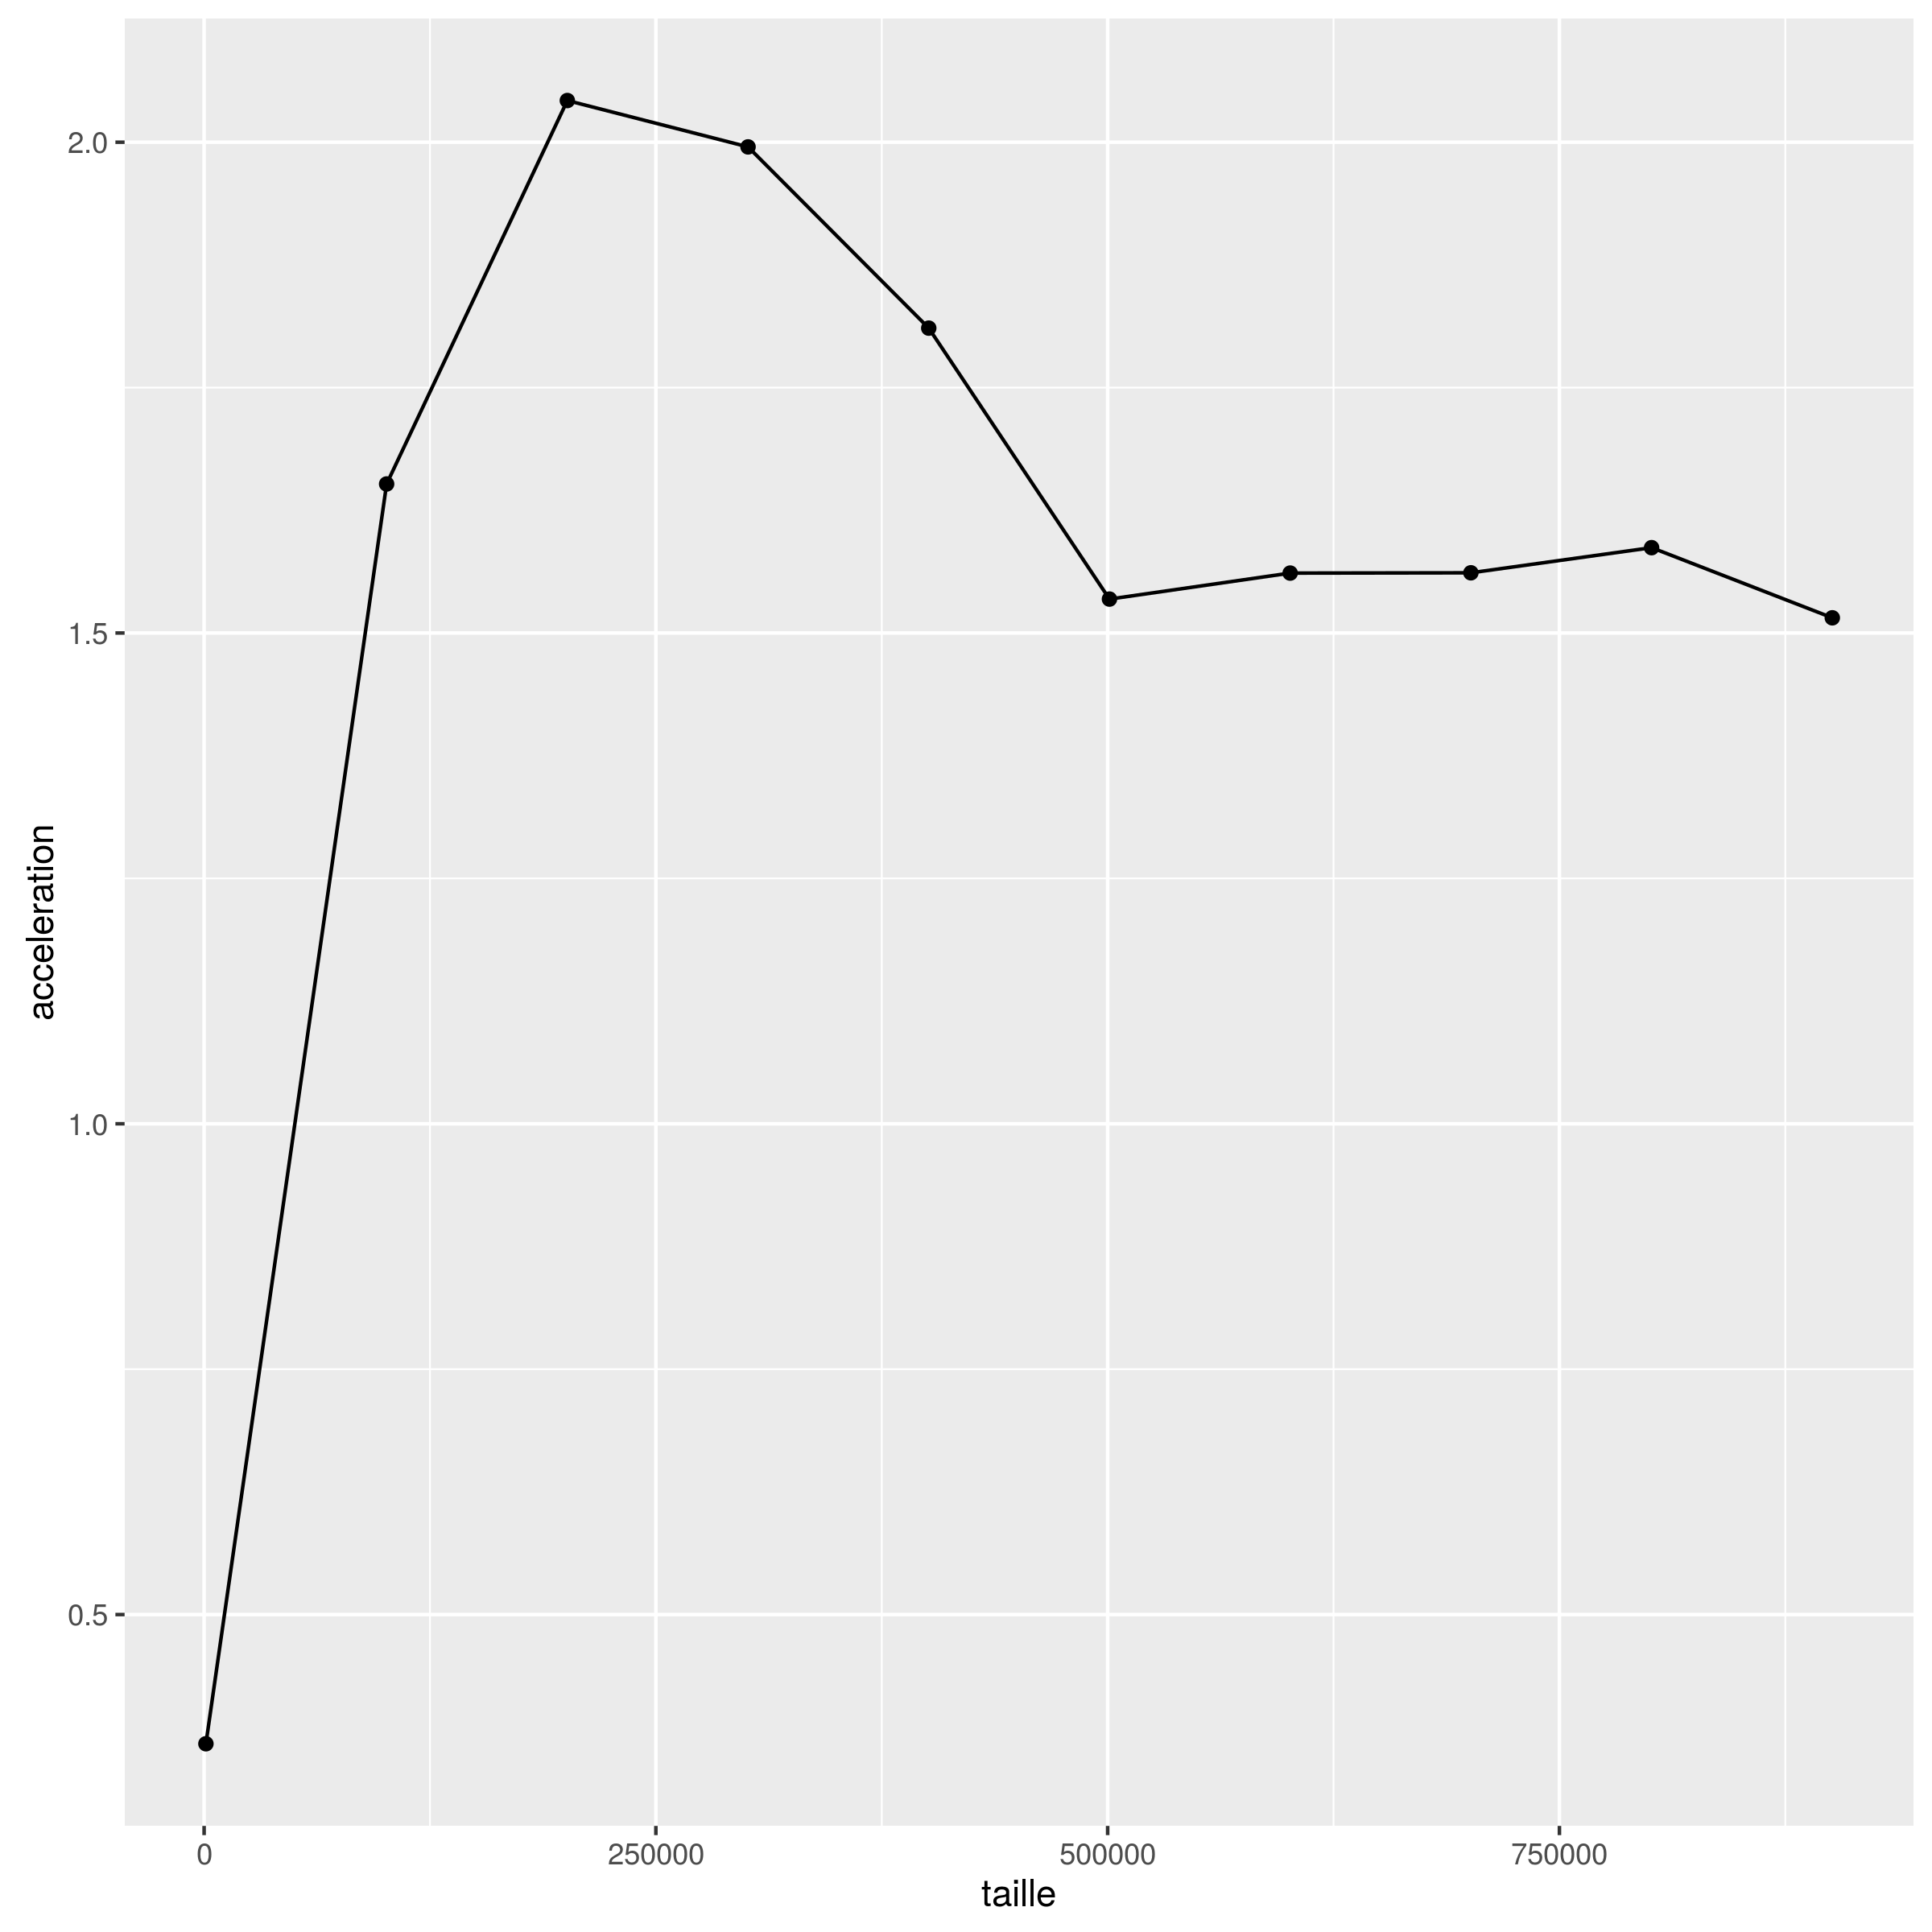
\includegraphics[scale=0.5] {graphes/global_temps_machine_accel7.png}
\end{figure}

Nous observons que pour des vecteurs allant d'une taille de 1000 \'el\'ements \`a 1000000 d'\'el\'ements, l'acc\'el\'eration est toujours sup\'erieur \`a 1. Nous observons aussi que l'acc\'el\'eration est la plus grande, pour des vecteurs d'une taille d'environ 200000 \'el\'ements. Pass\'e ce seuil, le niveau de l'acc\'el\'eration baisse et finit par tendre vers 1.5, pass\' le seuil des 500000 \'el\'ements.   


\subsection{Temps CPU cumul\'e de l'utilisateur}
\begin{figure}[H] \center
   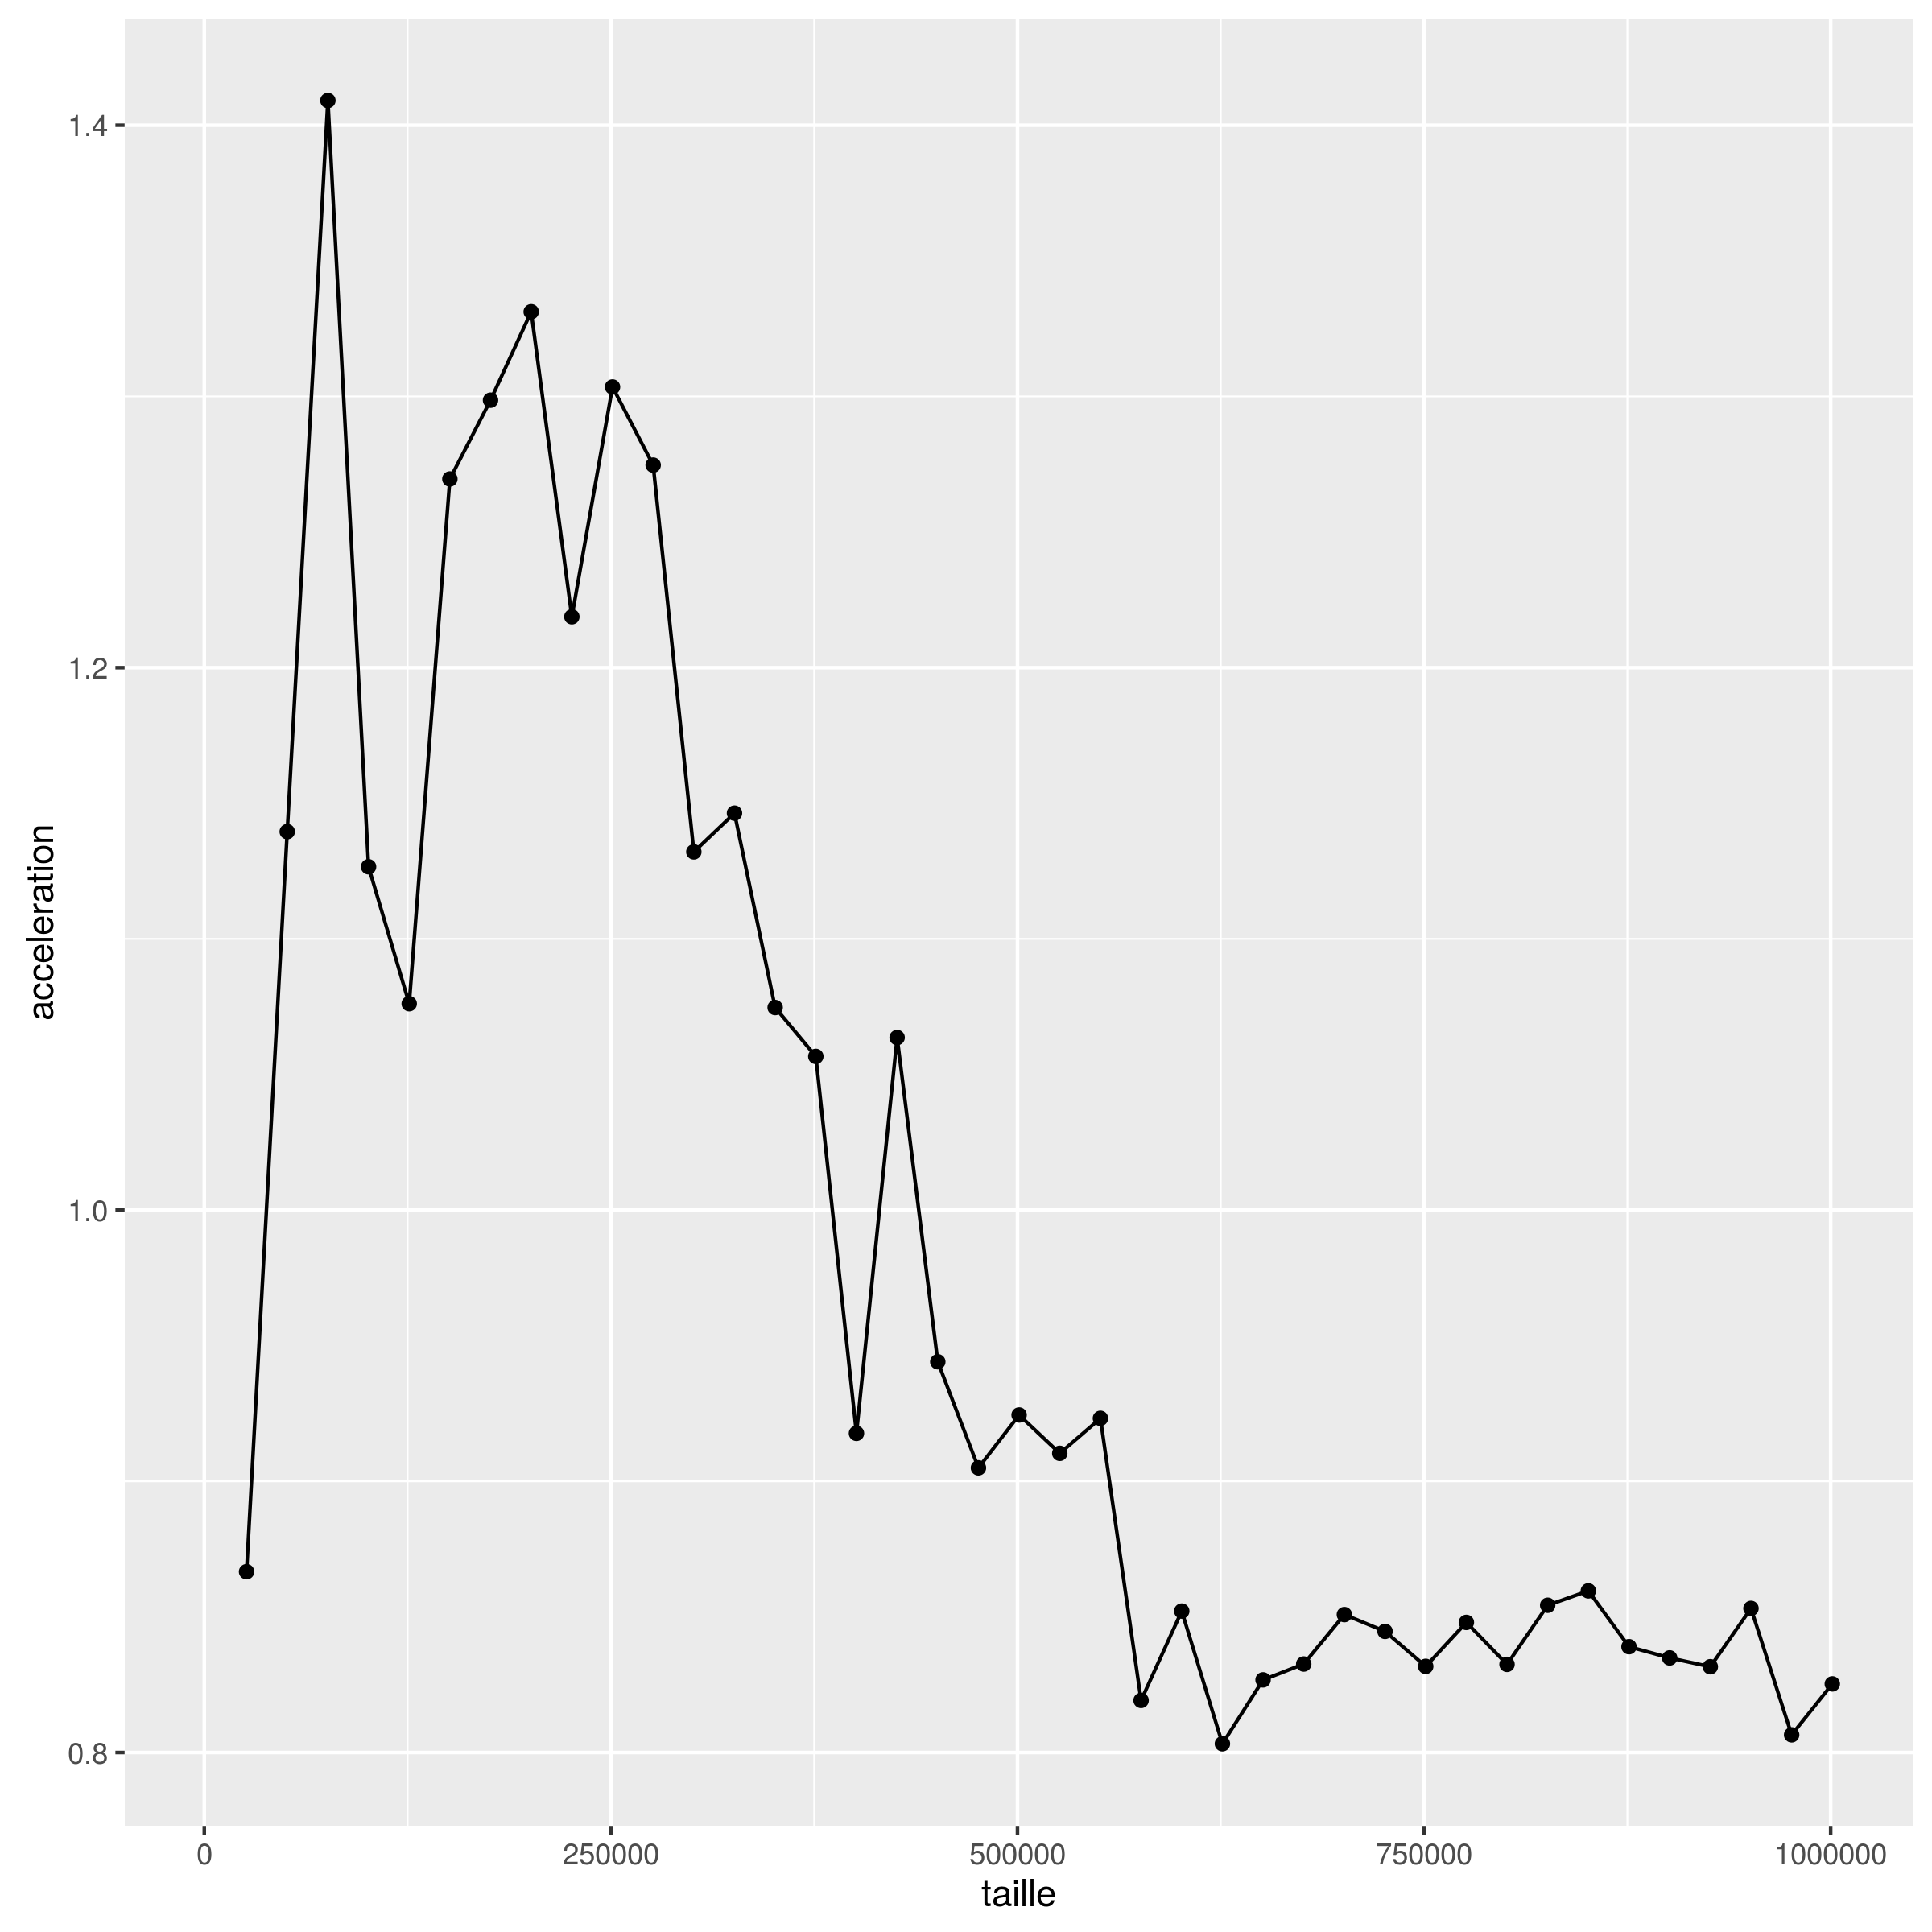
\includegraphics[scale=0.5] {graphes/temps_user_accel7.png}
\end{figure}
Nous observons que pour des vecteurs d'une taille inf\'erieur \`a 300000, l'acc\'el\'eration est sup\'erieur \`a 1. N\'eanmoins pass\'e ce seuil,  l'acc\'el\'eration est maintenant inf\'erieur \`a un, cela signifie que le temps CPU cumul\'e de l'utilisateur finit par \^{e}tre plus \'elev\'e avec 7 threads qu'en s\'equentiel. Cette acc\'el\'eration finit par tendre verss 0.8.


\section{Avec 8 threads}
\subsection{Temps d'ex\'ecution}

\begin{figure}[H] \center
   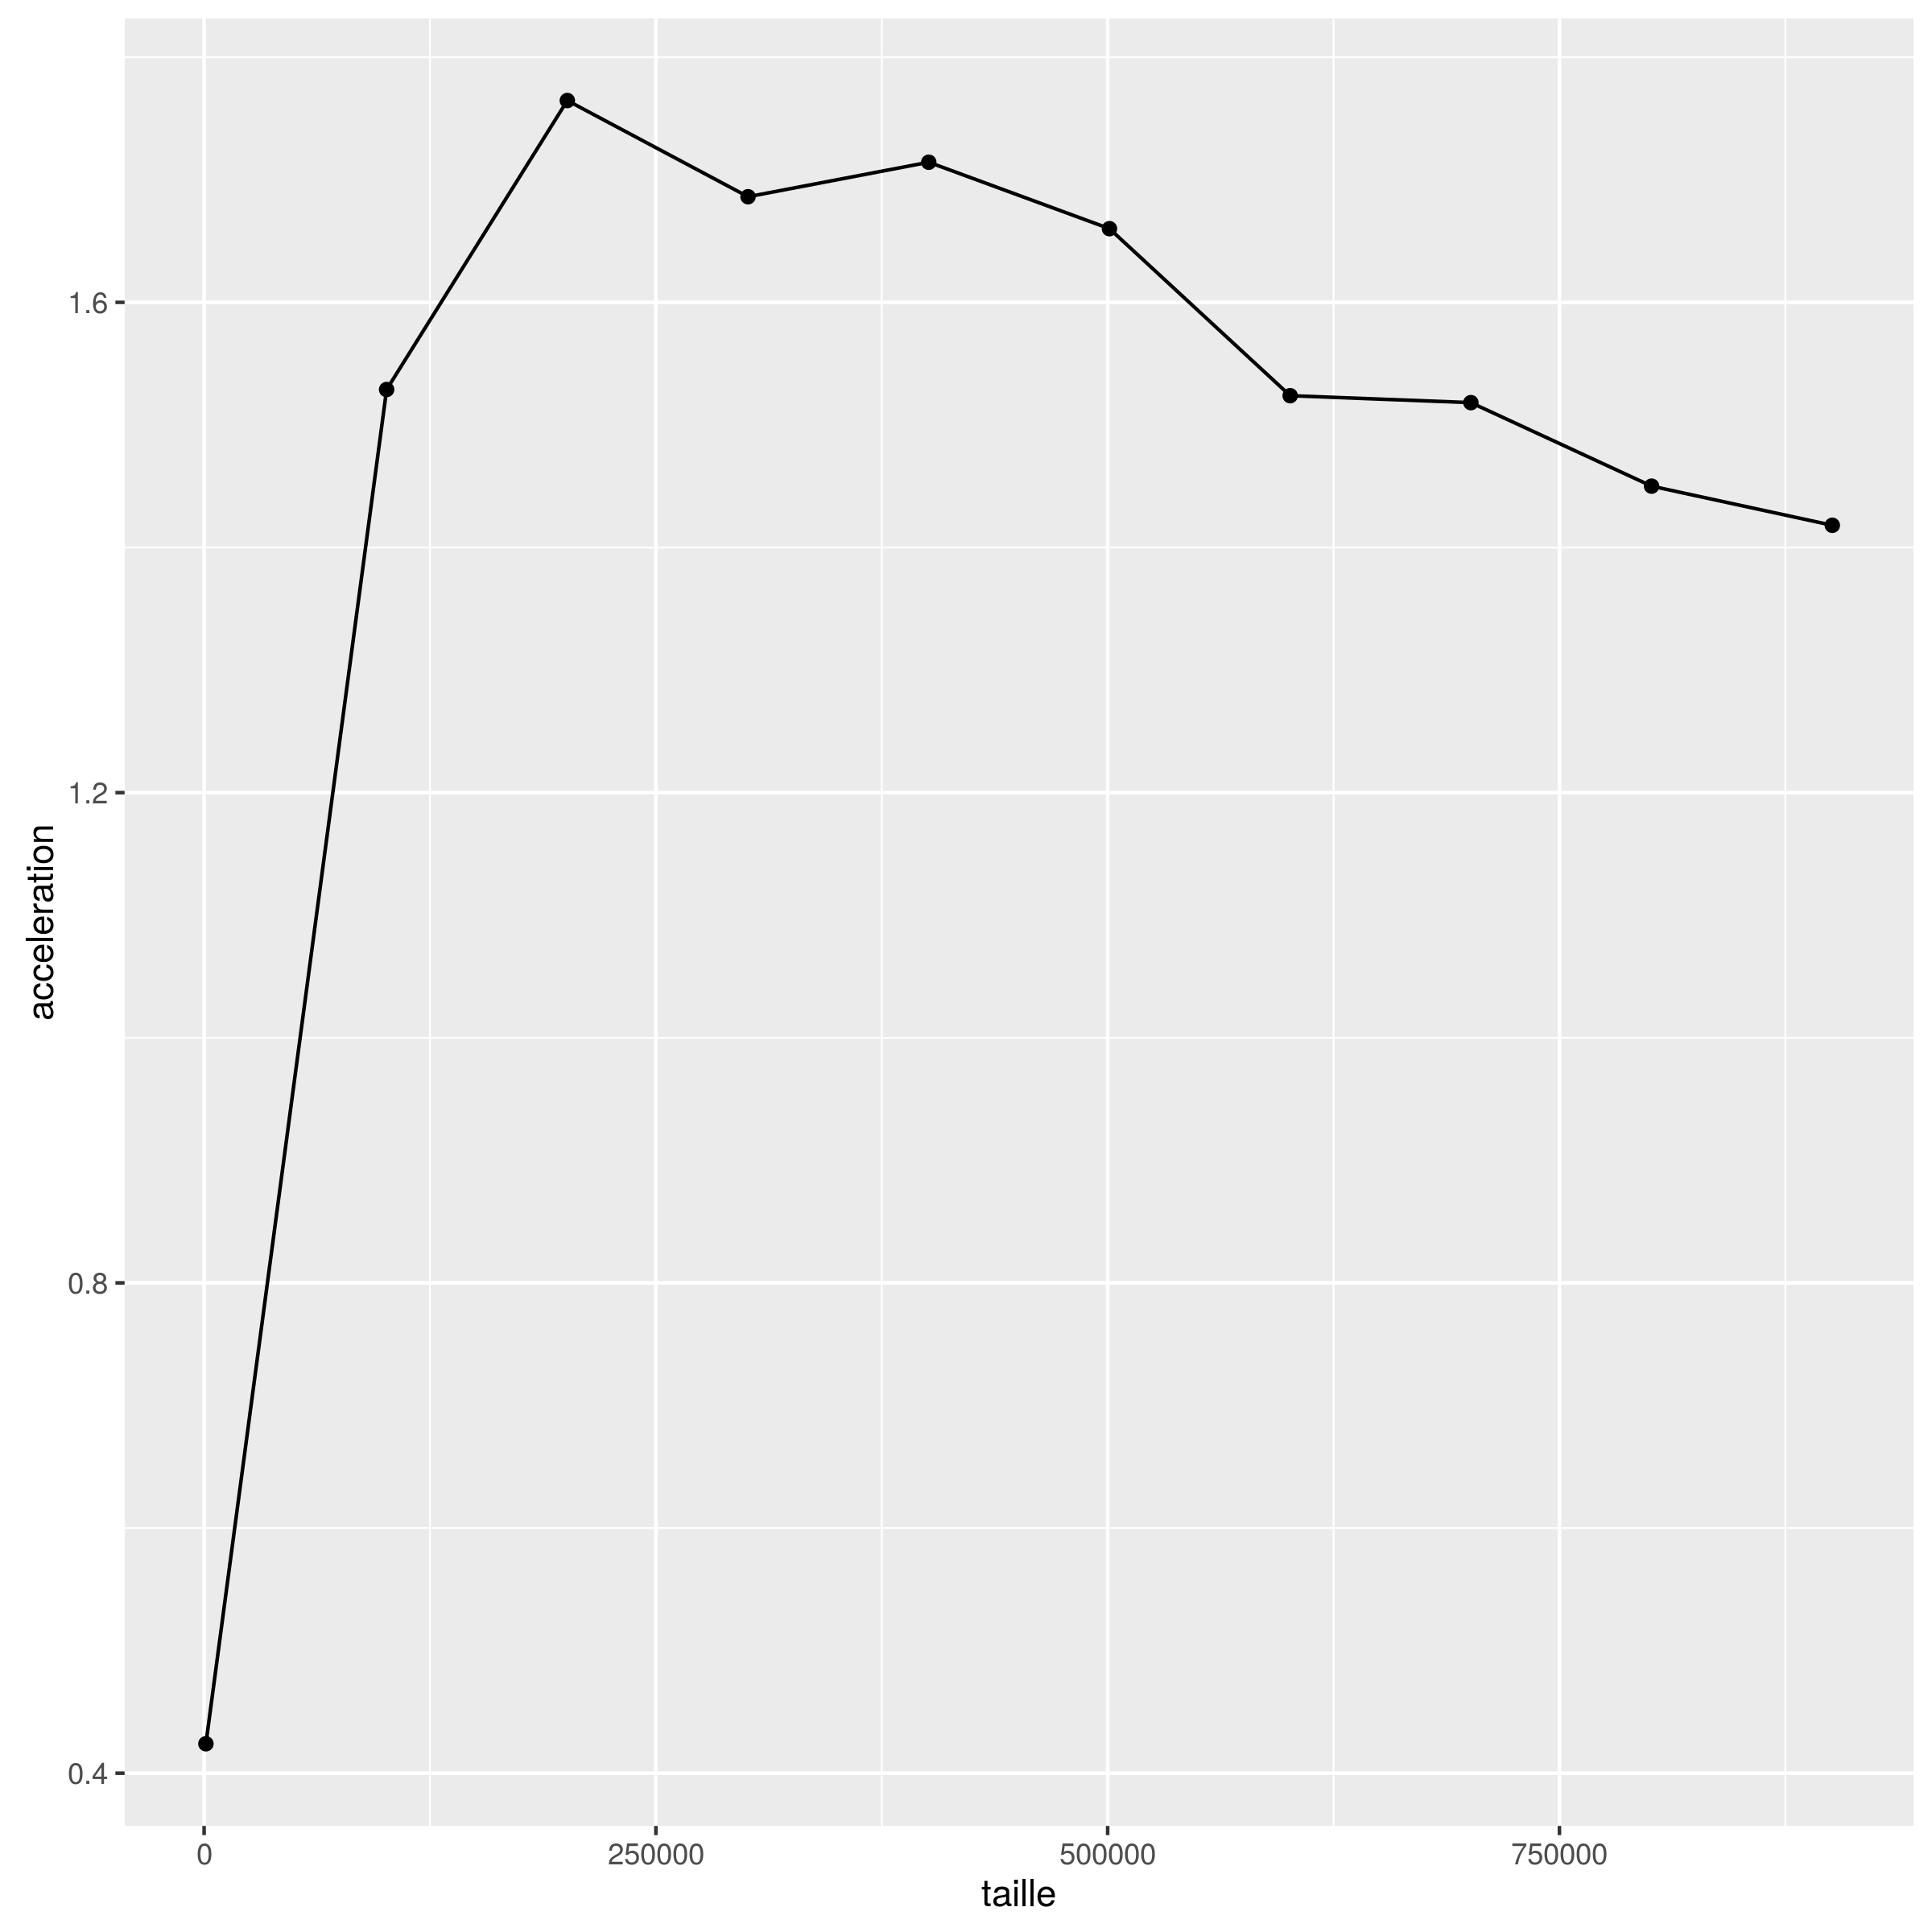
\includegraphics[scale=0.5] {graphes/global_temps_machine_accel8.png}
\end{figure}

Nous observons que pour des vecteurs allant d'une taille de 1000 \'el\'ements \`a 1000000 d'\'el\'ements, l'acc\'el\'eration est toujours sup\'erieur \`a 1. Nous observons aussi que l'acc\'el\'eration est la plus grande, pour des vecteurs d'une taille d'environ 200000 \'el\'ements. Pass\'e ce seuil, le niveau de l'acc\'el\'eration baisse et finit par tendre vers 1.4, pass\' le seuil des 800000 \'el\'ements.   


\subsection{Temps CPU cumul\'e de l'utilisateur}
\begin{figure}[H] \center
   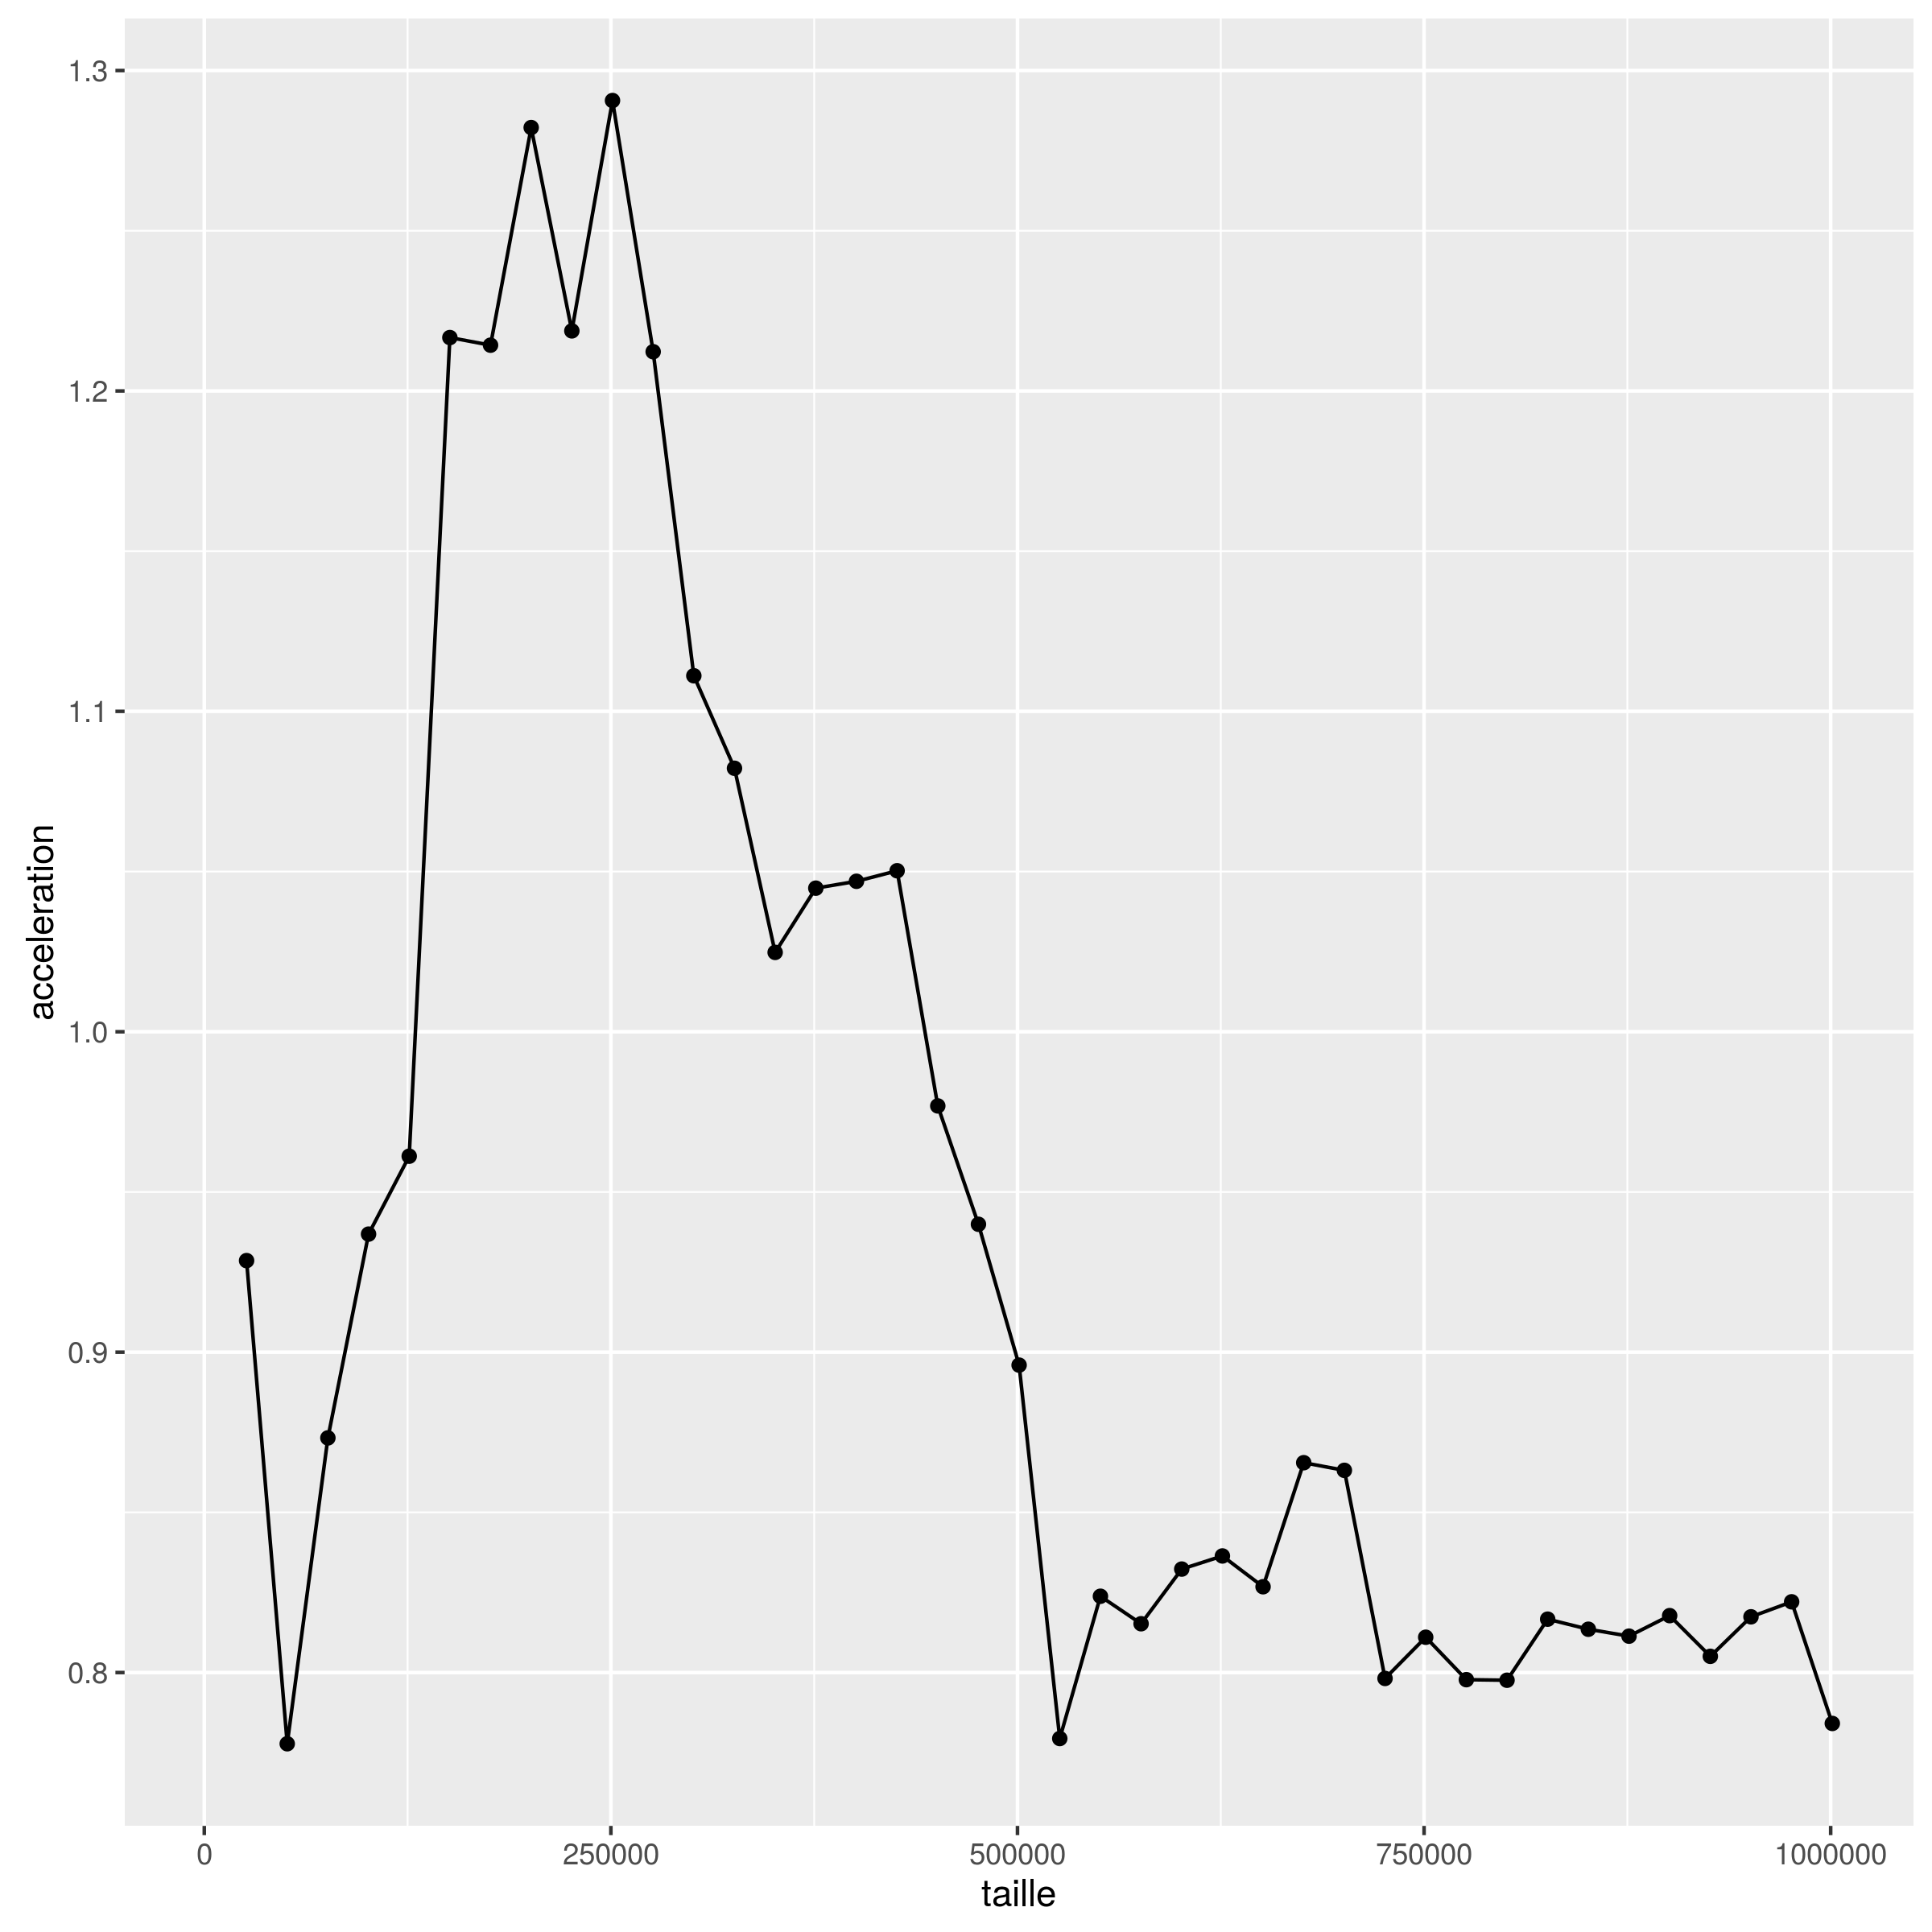
\includegraphics[scale=0.5] {graphes/temps_user_accel8.png}
\end{figure}
Nous observons que pour des vecteurs d'une taille inf\'erieur \`a 400000, l'acc\'el\'eration est sup\'erieur \`a 1. N\'eanmoins pass\'e ce seuil,  l'acc\'el\'eration est maintenant inf\'erieur \`a un, cela signifie que le temps CPU cumul\'e de l'utilisateur finit par \^{e}tre plus \'elev\'e avec 8 threads qu'en s\'equentiel. Cette acc\'el\'eration finit par tendre verss 0.7.


\section{Avec 9 threads}
\subsection{Temps d'ex\'ecution}

\begin{figure}[H] \center
   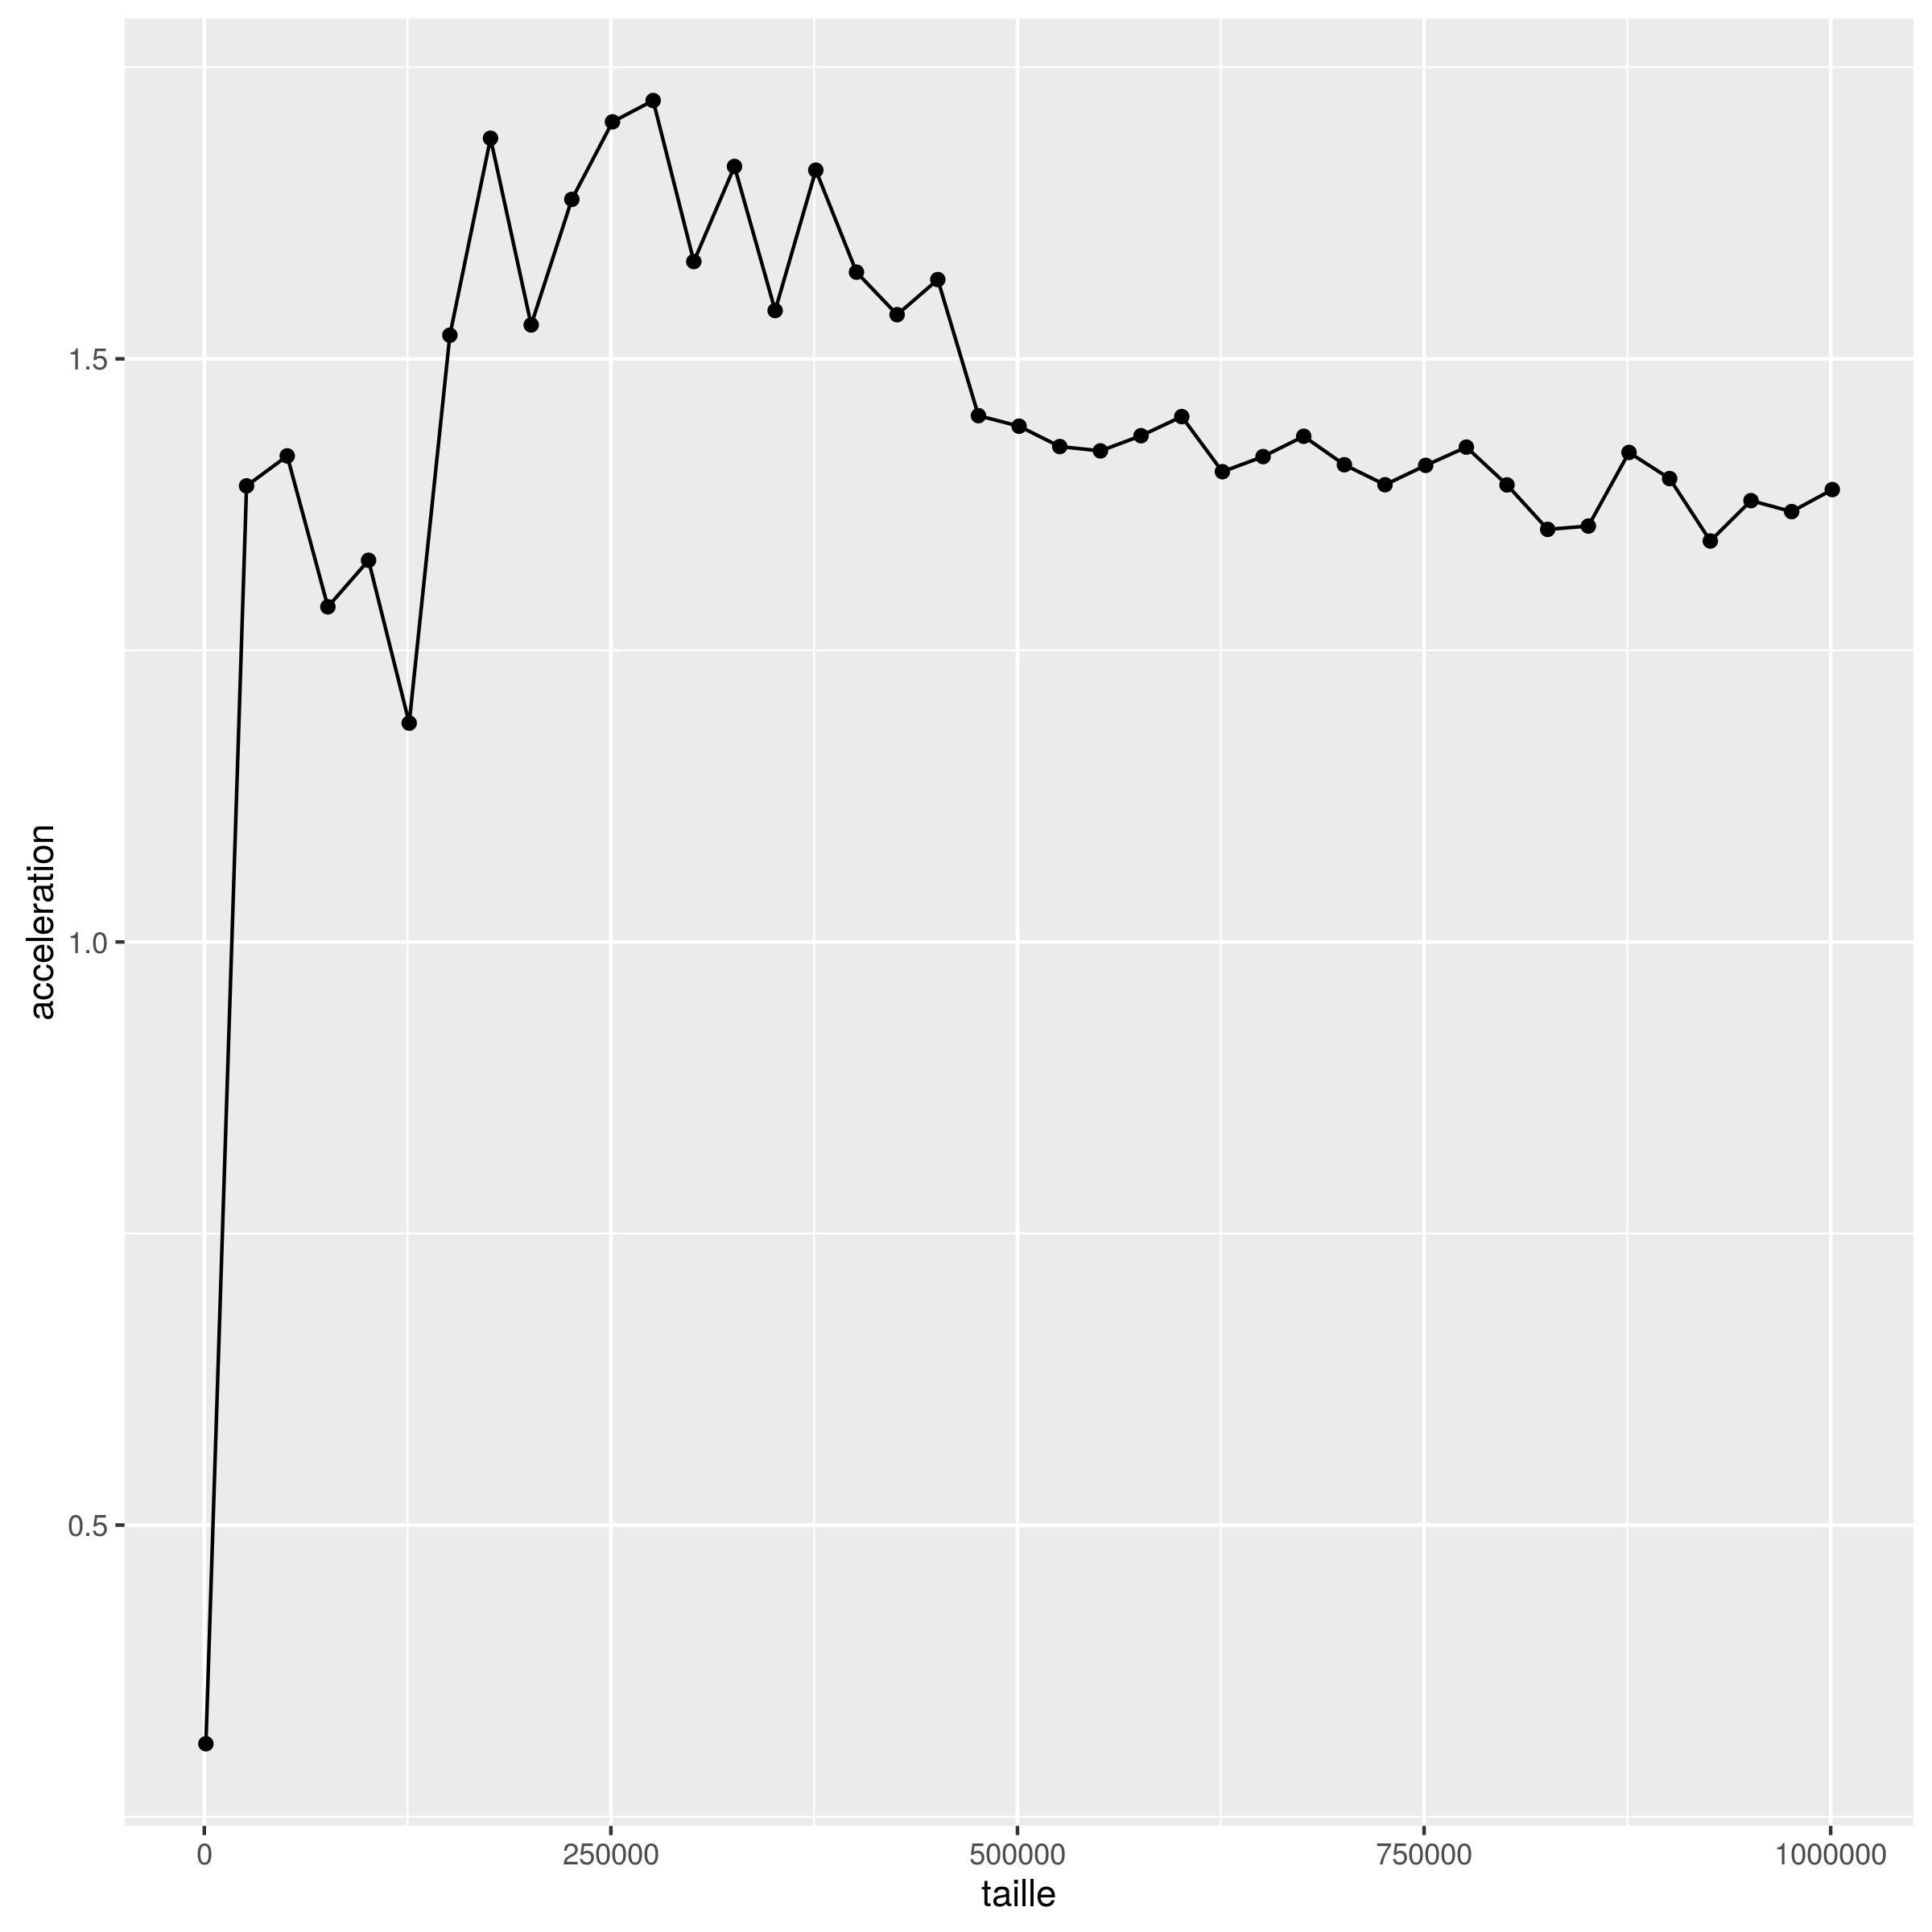
\includegraphics[scale=0.5] {graphes/global_temps_machine_accel9.png}
\end{figure}

Nous observons que pour des vecteurs allant d'une taille de 1000 \'el\'ements \`a 1000000 d'\'el\'ements, l'acc\'el\'eration est toujours sup\'erieur \`a 1. Nous observons aussi que l'acc\'el\'eration est la plus grande, pour des vecteurs d'une taille d'environ 400000 \'el\'ements. Pass\'e ce seuil, le niveau de l'acc\'el\'eration baisse et finit par tendre vers 1.4, pass\' le seuil des 500000 \'el\'ements.   


\subsection{Temps CPU cumul\'e de l'utilisateur}
\begin{figure}[H] \center
   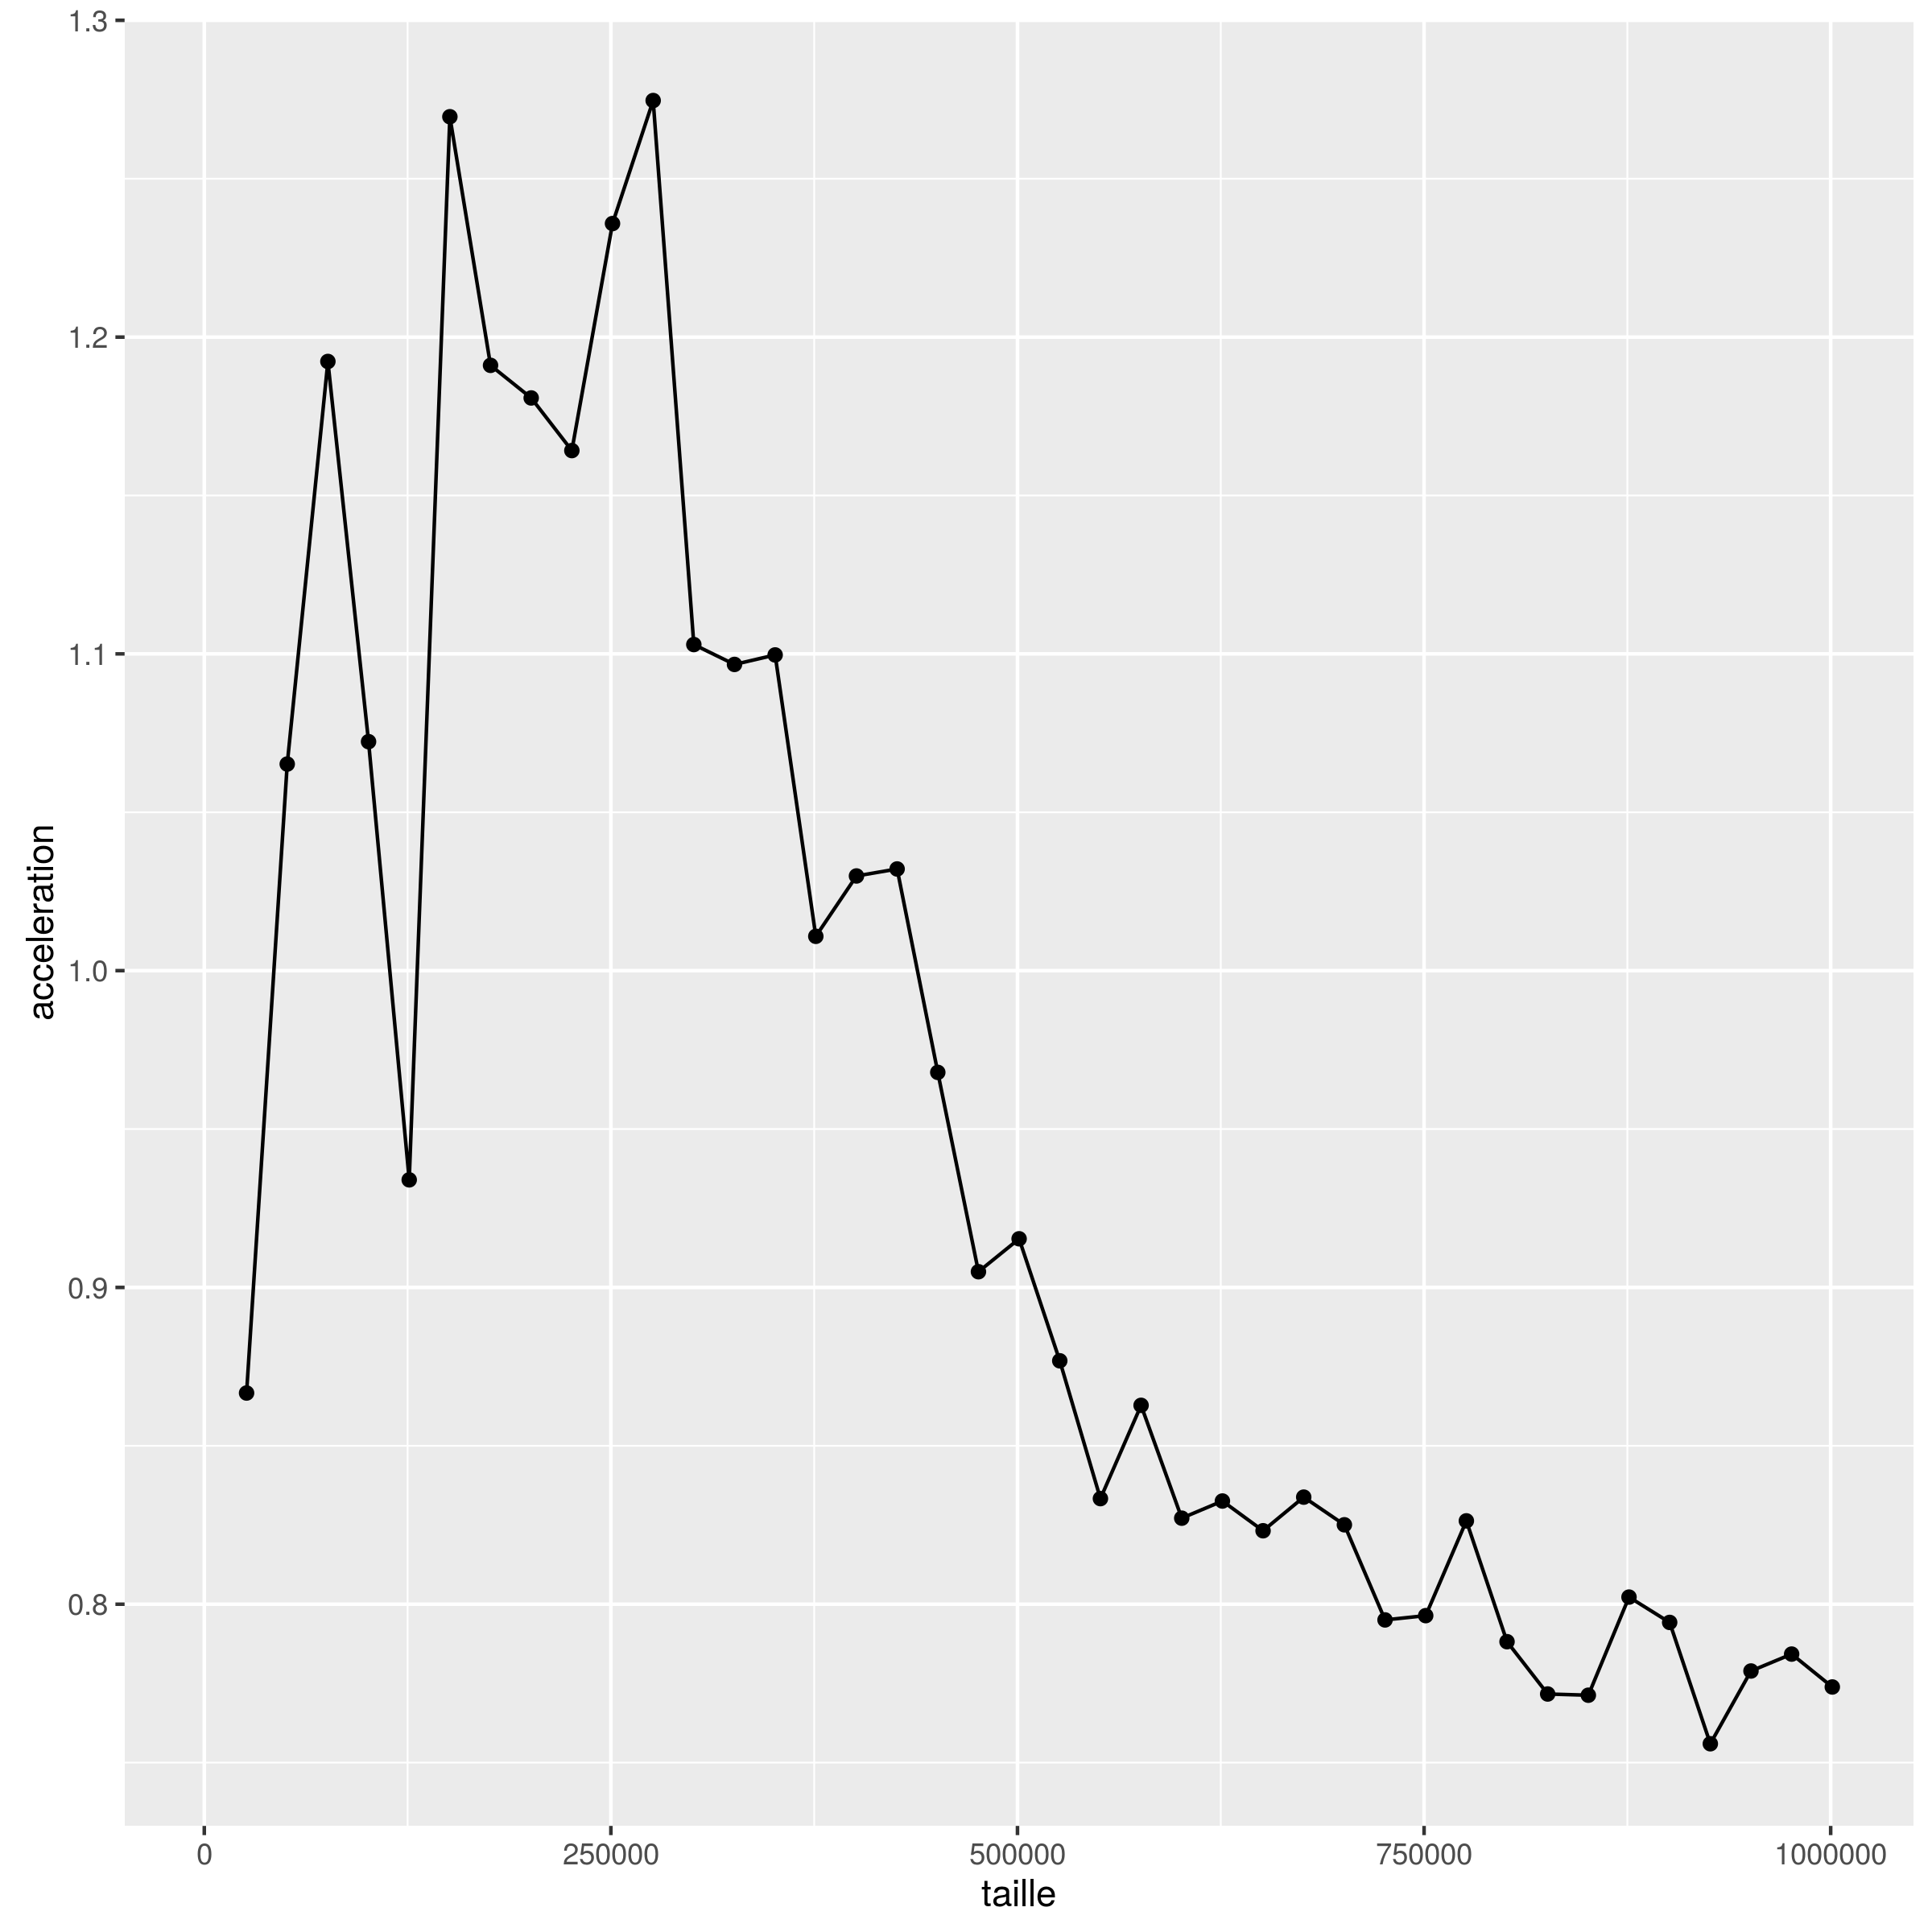
\includegraphics[scale=0.5] {graphes/temps_user_accel9.png}
\end{figure}
Nous observons que pour des vecteurs d'une taille inf\'erieur \`a 450000, l'acc\'el\'eration est sup\'erieur \`a 1. N\'eanmoins pass\'e ce seuil,  l'acc\'el\'eration est maintenant inf\'erieur \`a un, cela signifie que le temps CPU cumul\'e de l'utilisateur finit par \^{e}tre plus \'elev\'e avec 9 threads qu'en s\'equentiel. Cette acc\'el\'eration finit par tendre verss 0.7.


\section{Avec 10 threads}
\subsection{Temps d'ex\'ecution}

\begin{figure}[H] \center
   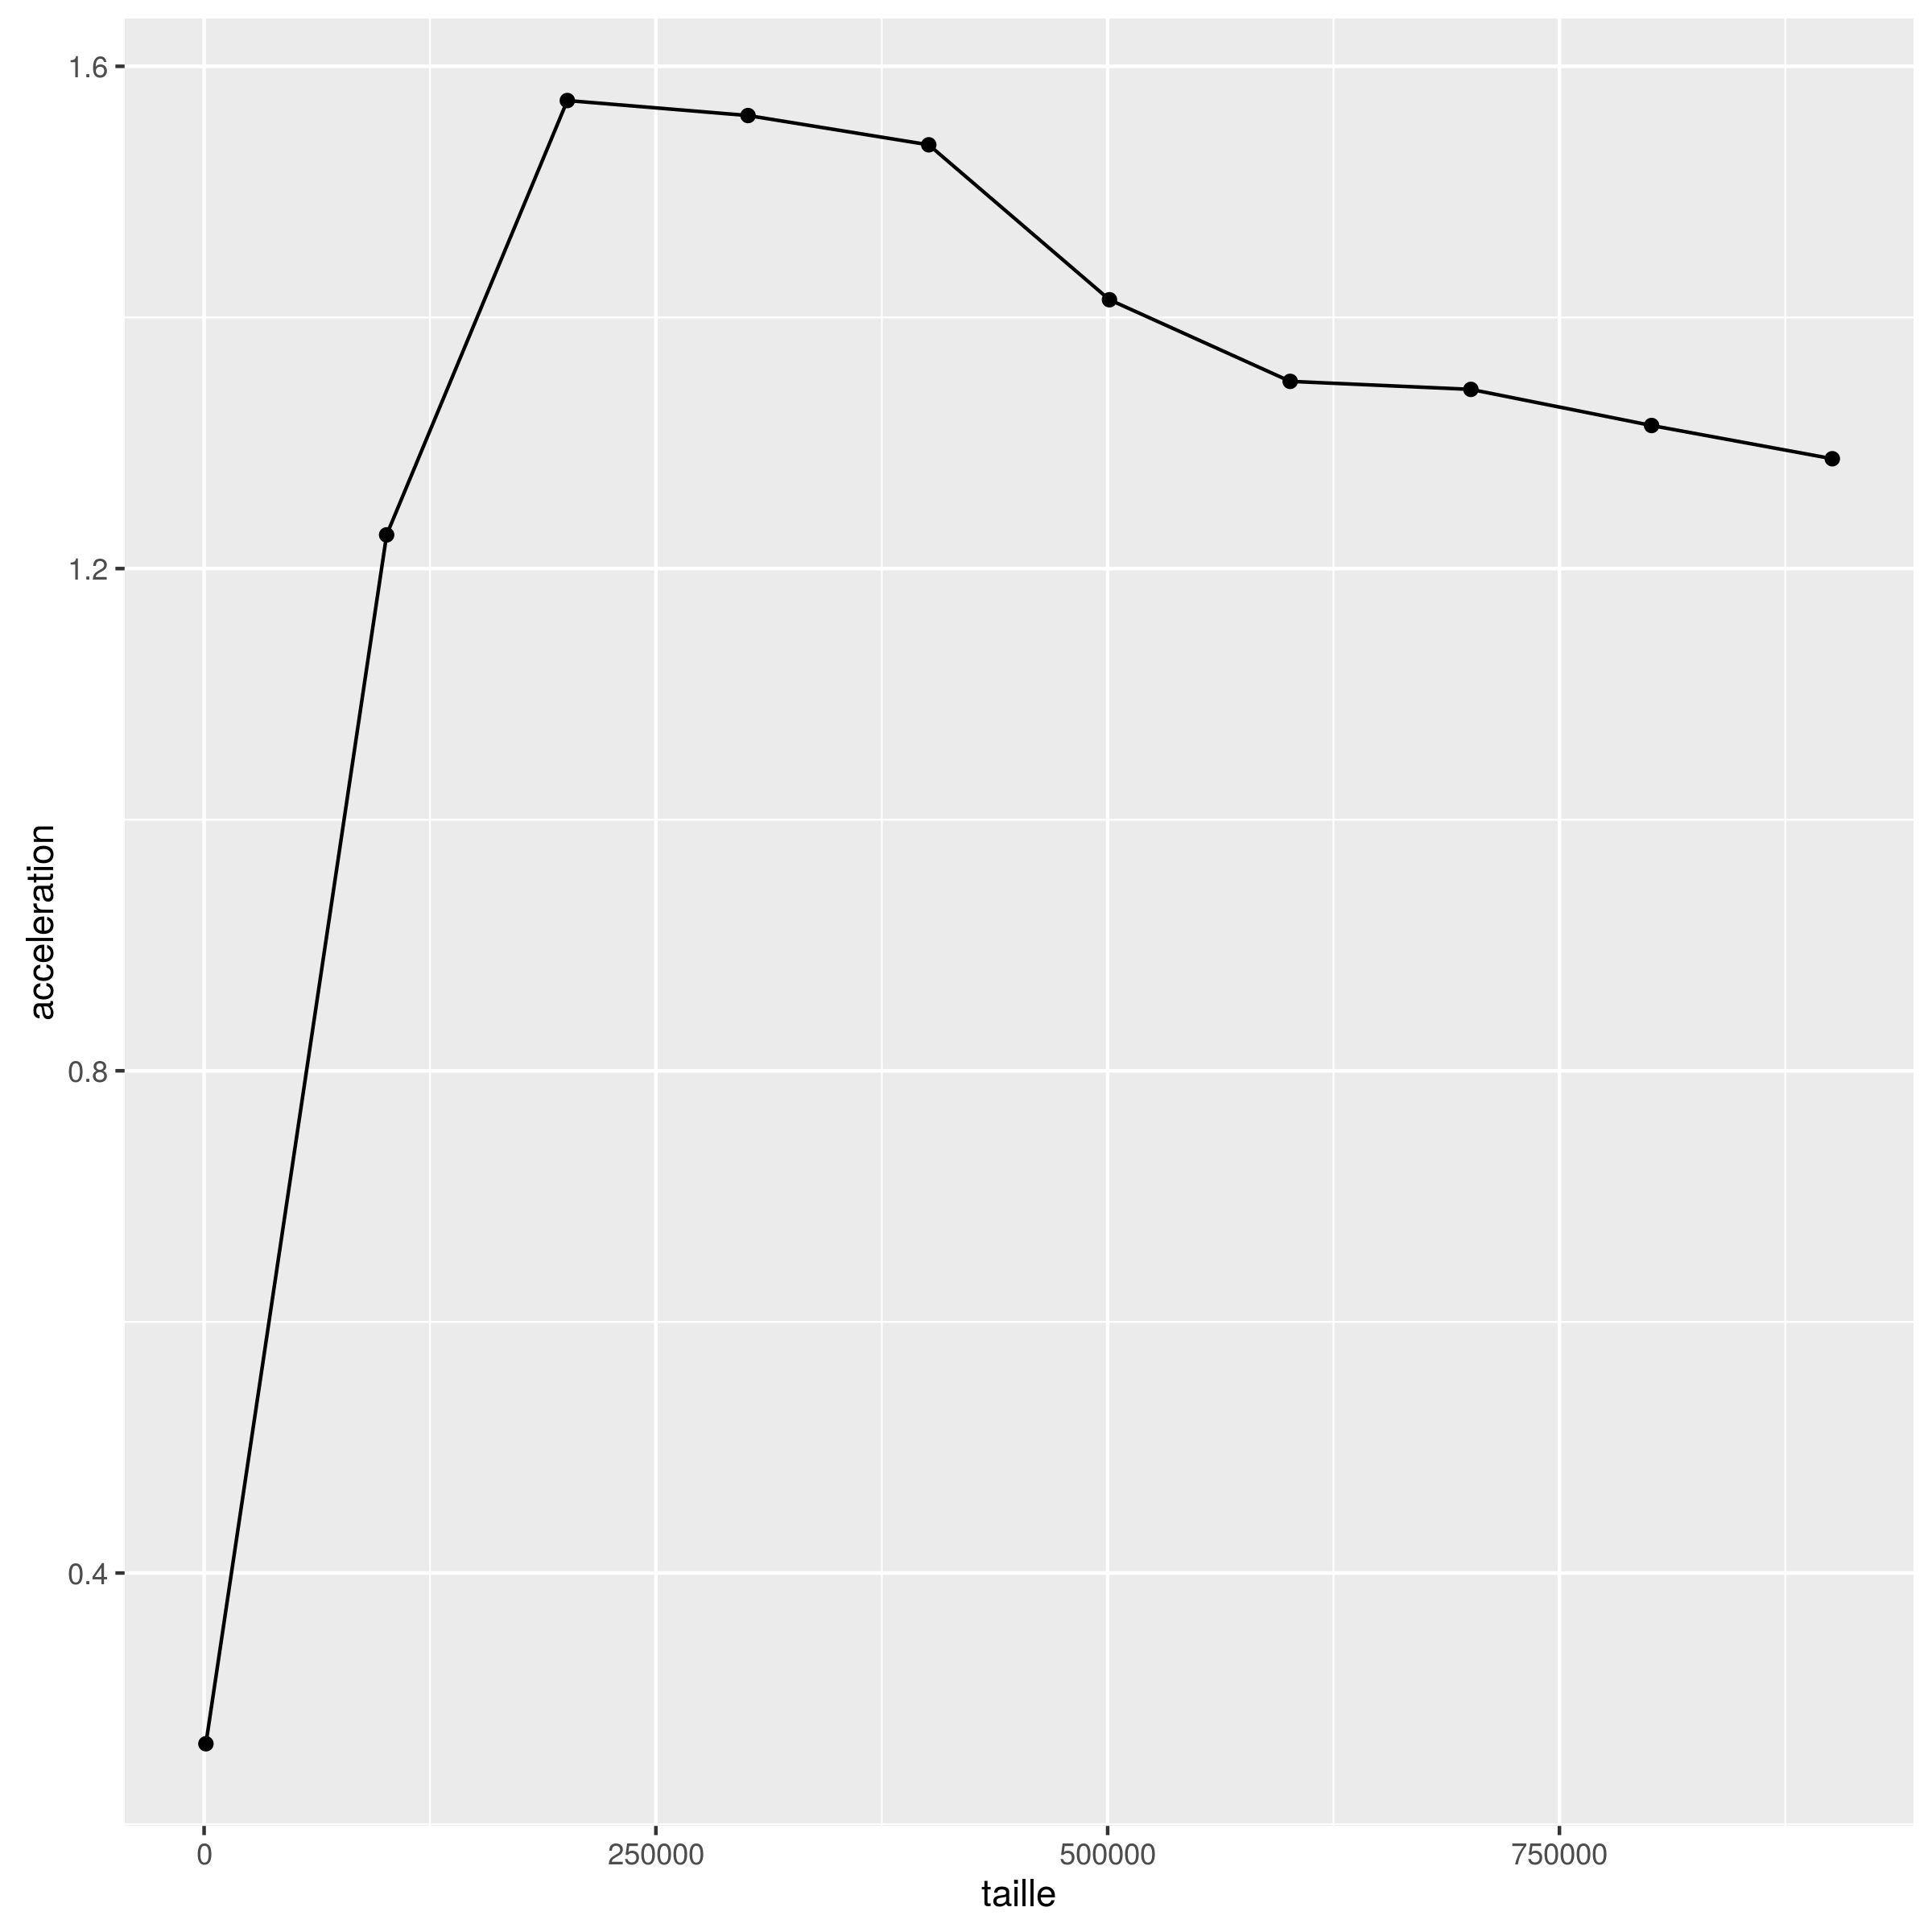
\includegraphics[scale=0.5] {graphes/global_temps_machine_accel10.png}
\end{figure}

Nous observons que pour des vecteurs allant d'une taille de 1000 \'el\'ements \`a 1000000 d'\'el\'ements, l'acc\'el\'eration est toujours sup\'erieur \`a 1. Nous observons aussi que l'acc\'el\'eration est la plus grande, pour des vecteurs d'une taille d'environ 250000 \'el\'ements. Pass\'e ce seuil, le niveau de l'acc\'el\'eration baisse et finit par tendre vers 1.3, pass\' le seuil des 550000 \'el\'ements.   


\subsection{Temps CPU cumul\'e de l'utilisateur}
\begin{figure}[H] \center
   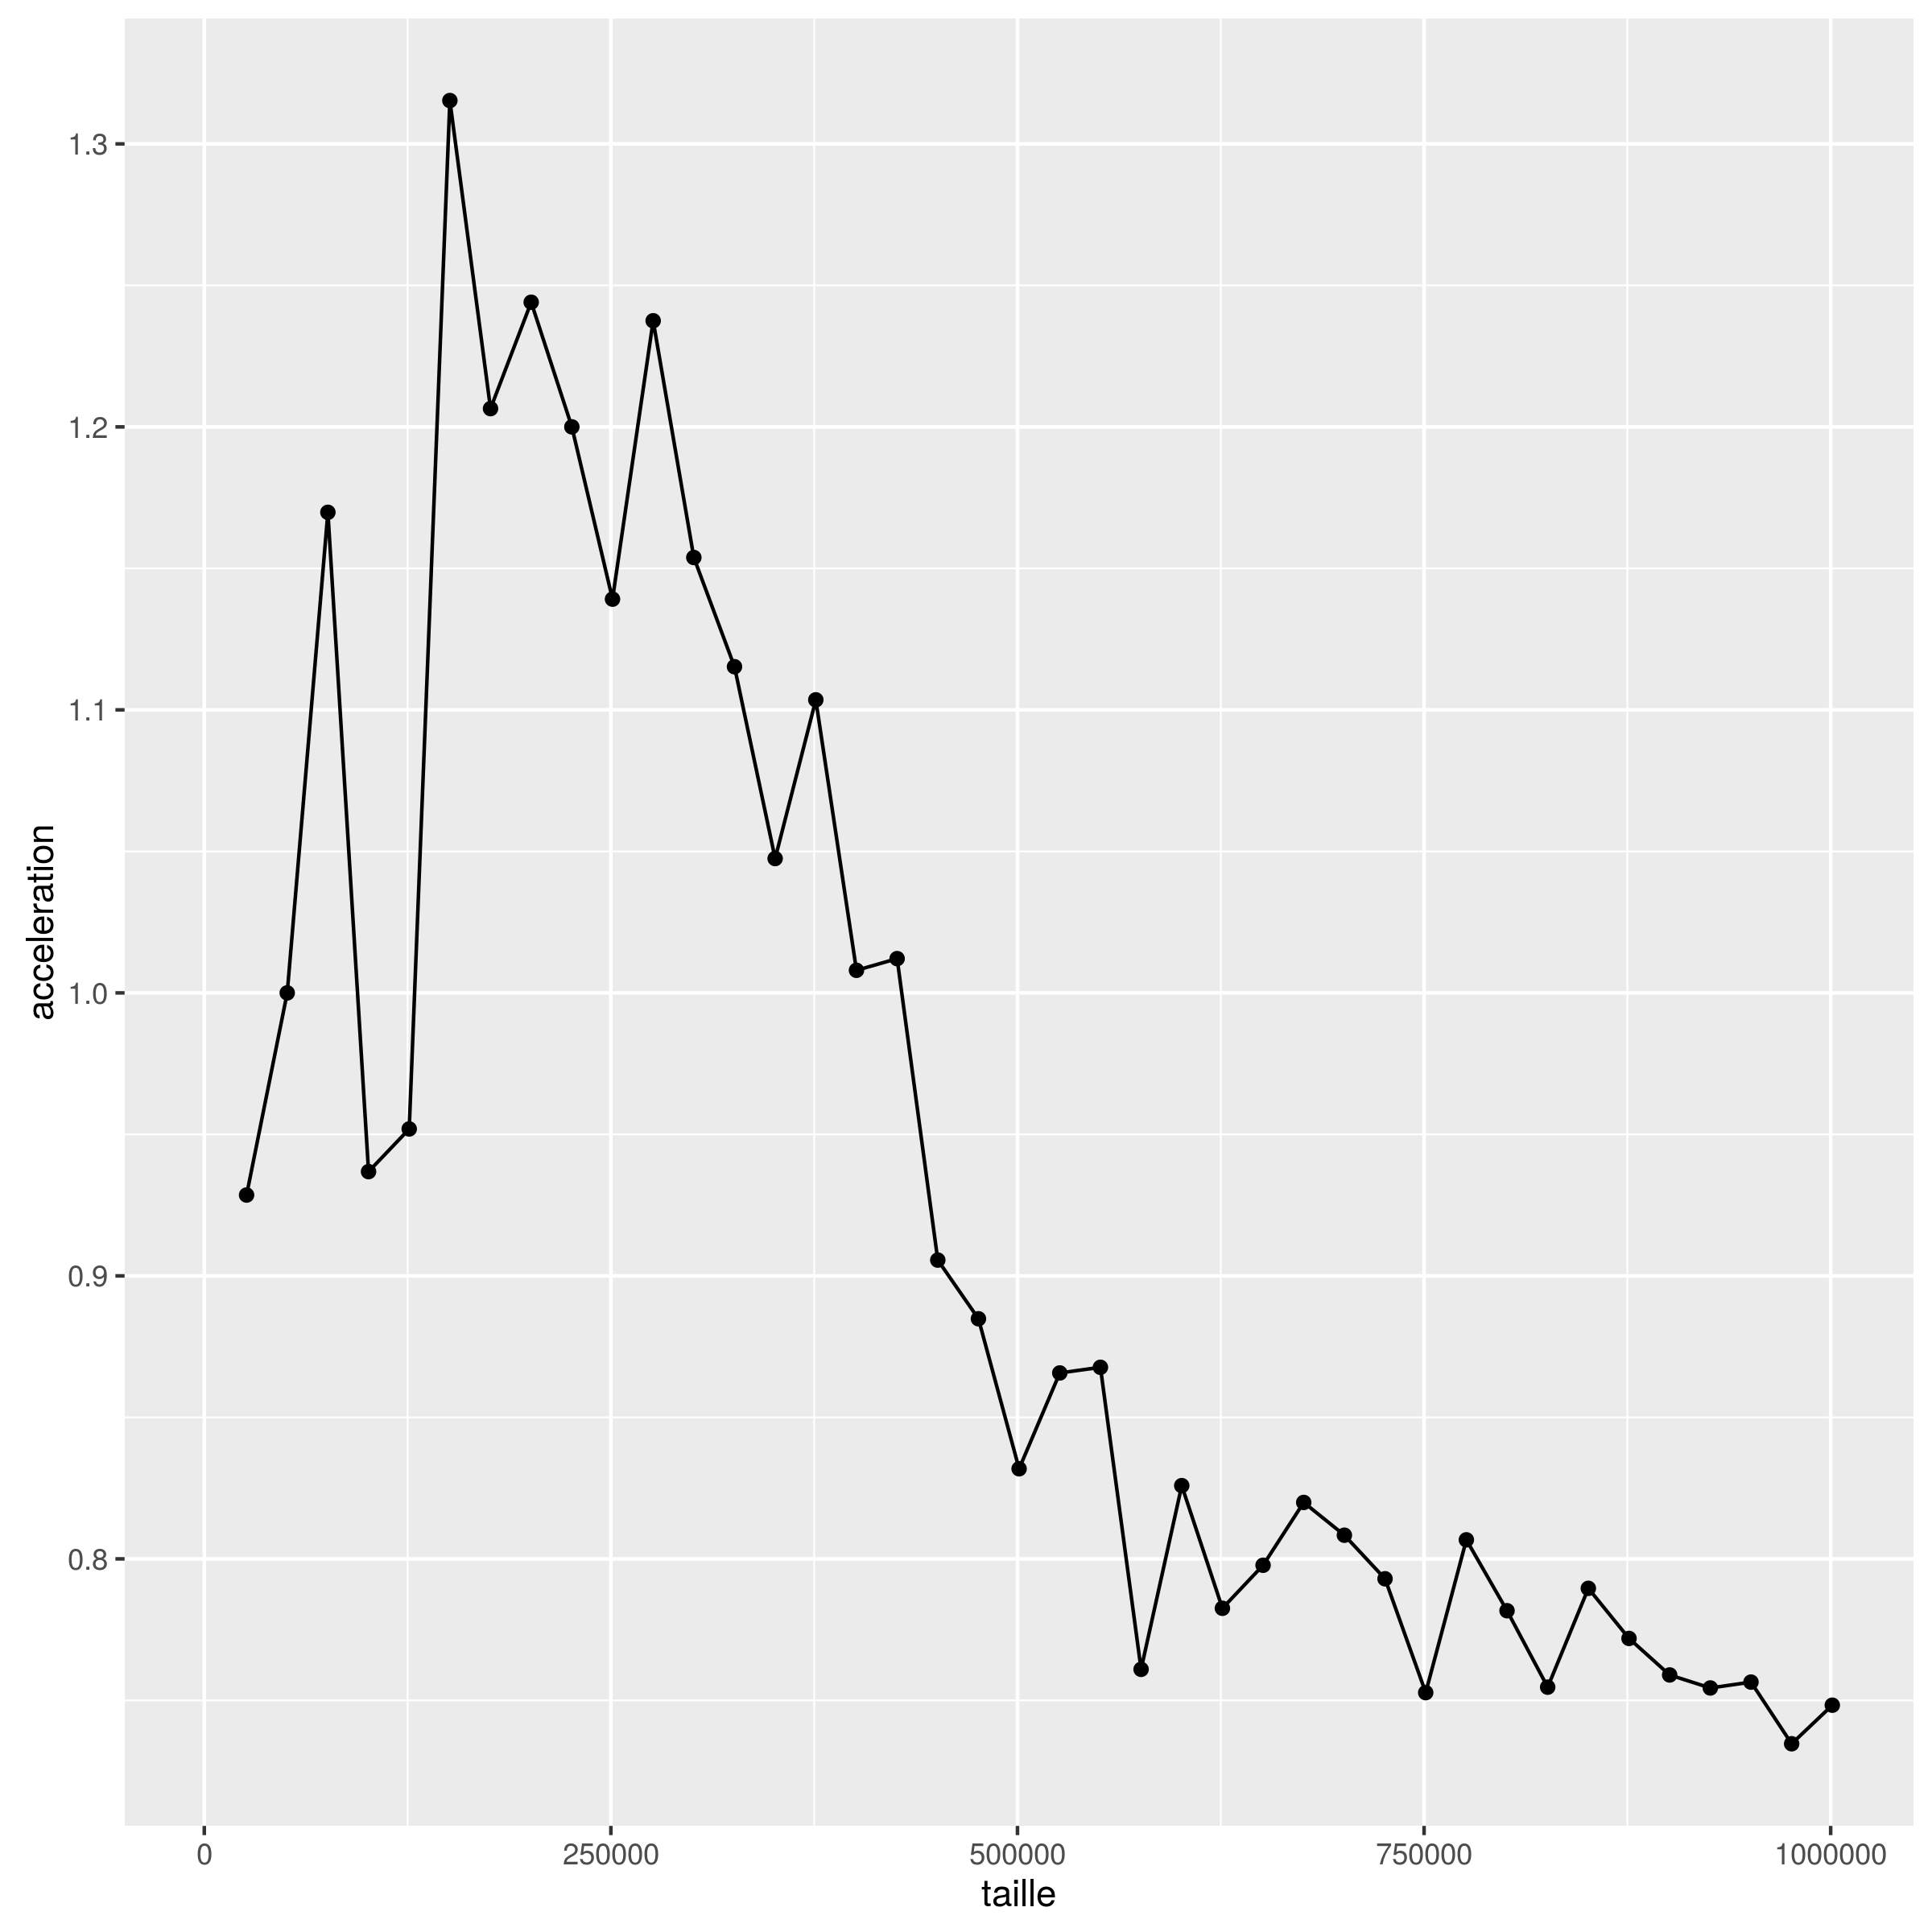
\includegraphics[scale=0.5] {graphes/temps_user_accel10.png}
\end{figure}
Nous observons que pour des vecteurs d'une taille inf\'erieur \`a 450000, l'acc\'el\'eration est sup\'erieur \`a 1. N\'eanmoins pass\'e ce seuil,  l'acc\'el\'eration est maintenant inf\'erieur \`a un, cela signifie que le temps CPU cumul\'e de l'utilisateur finit par \^{e}tre plus \'elev\'e avec 10 threads qu'en s\'equentiel. Cette acc\'el\'eration finit par tendre verss 0.7.


\section{Avec 11 threads}
\subsection{Temps d'ex\'ecution}

\begin{figure}[H] \center
   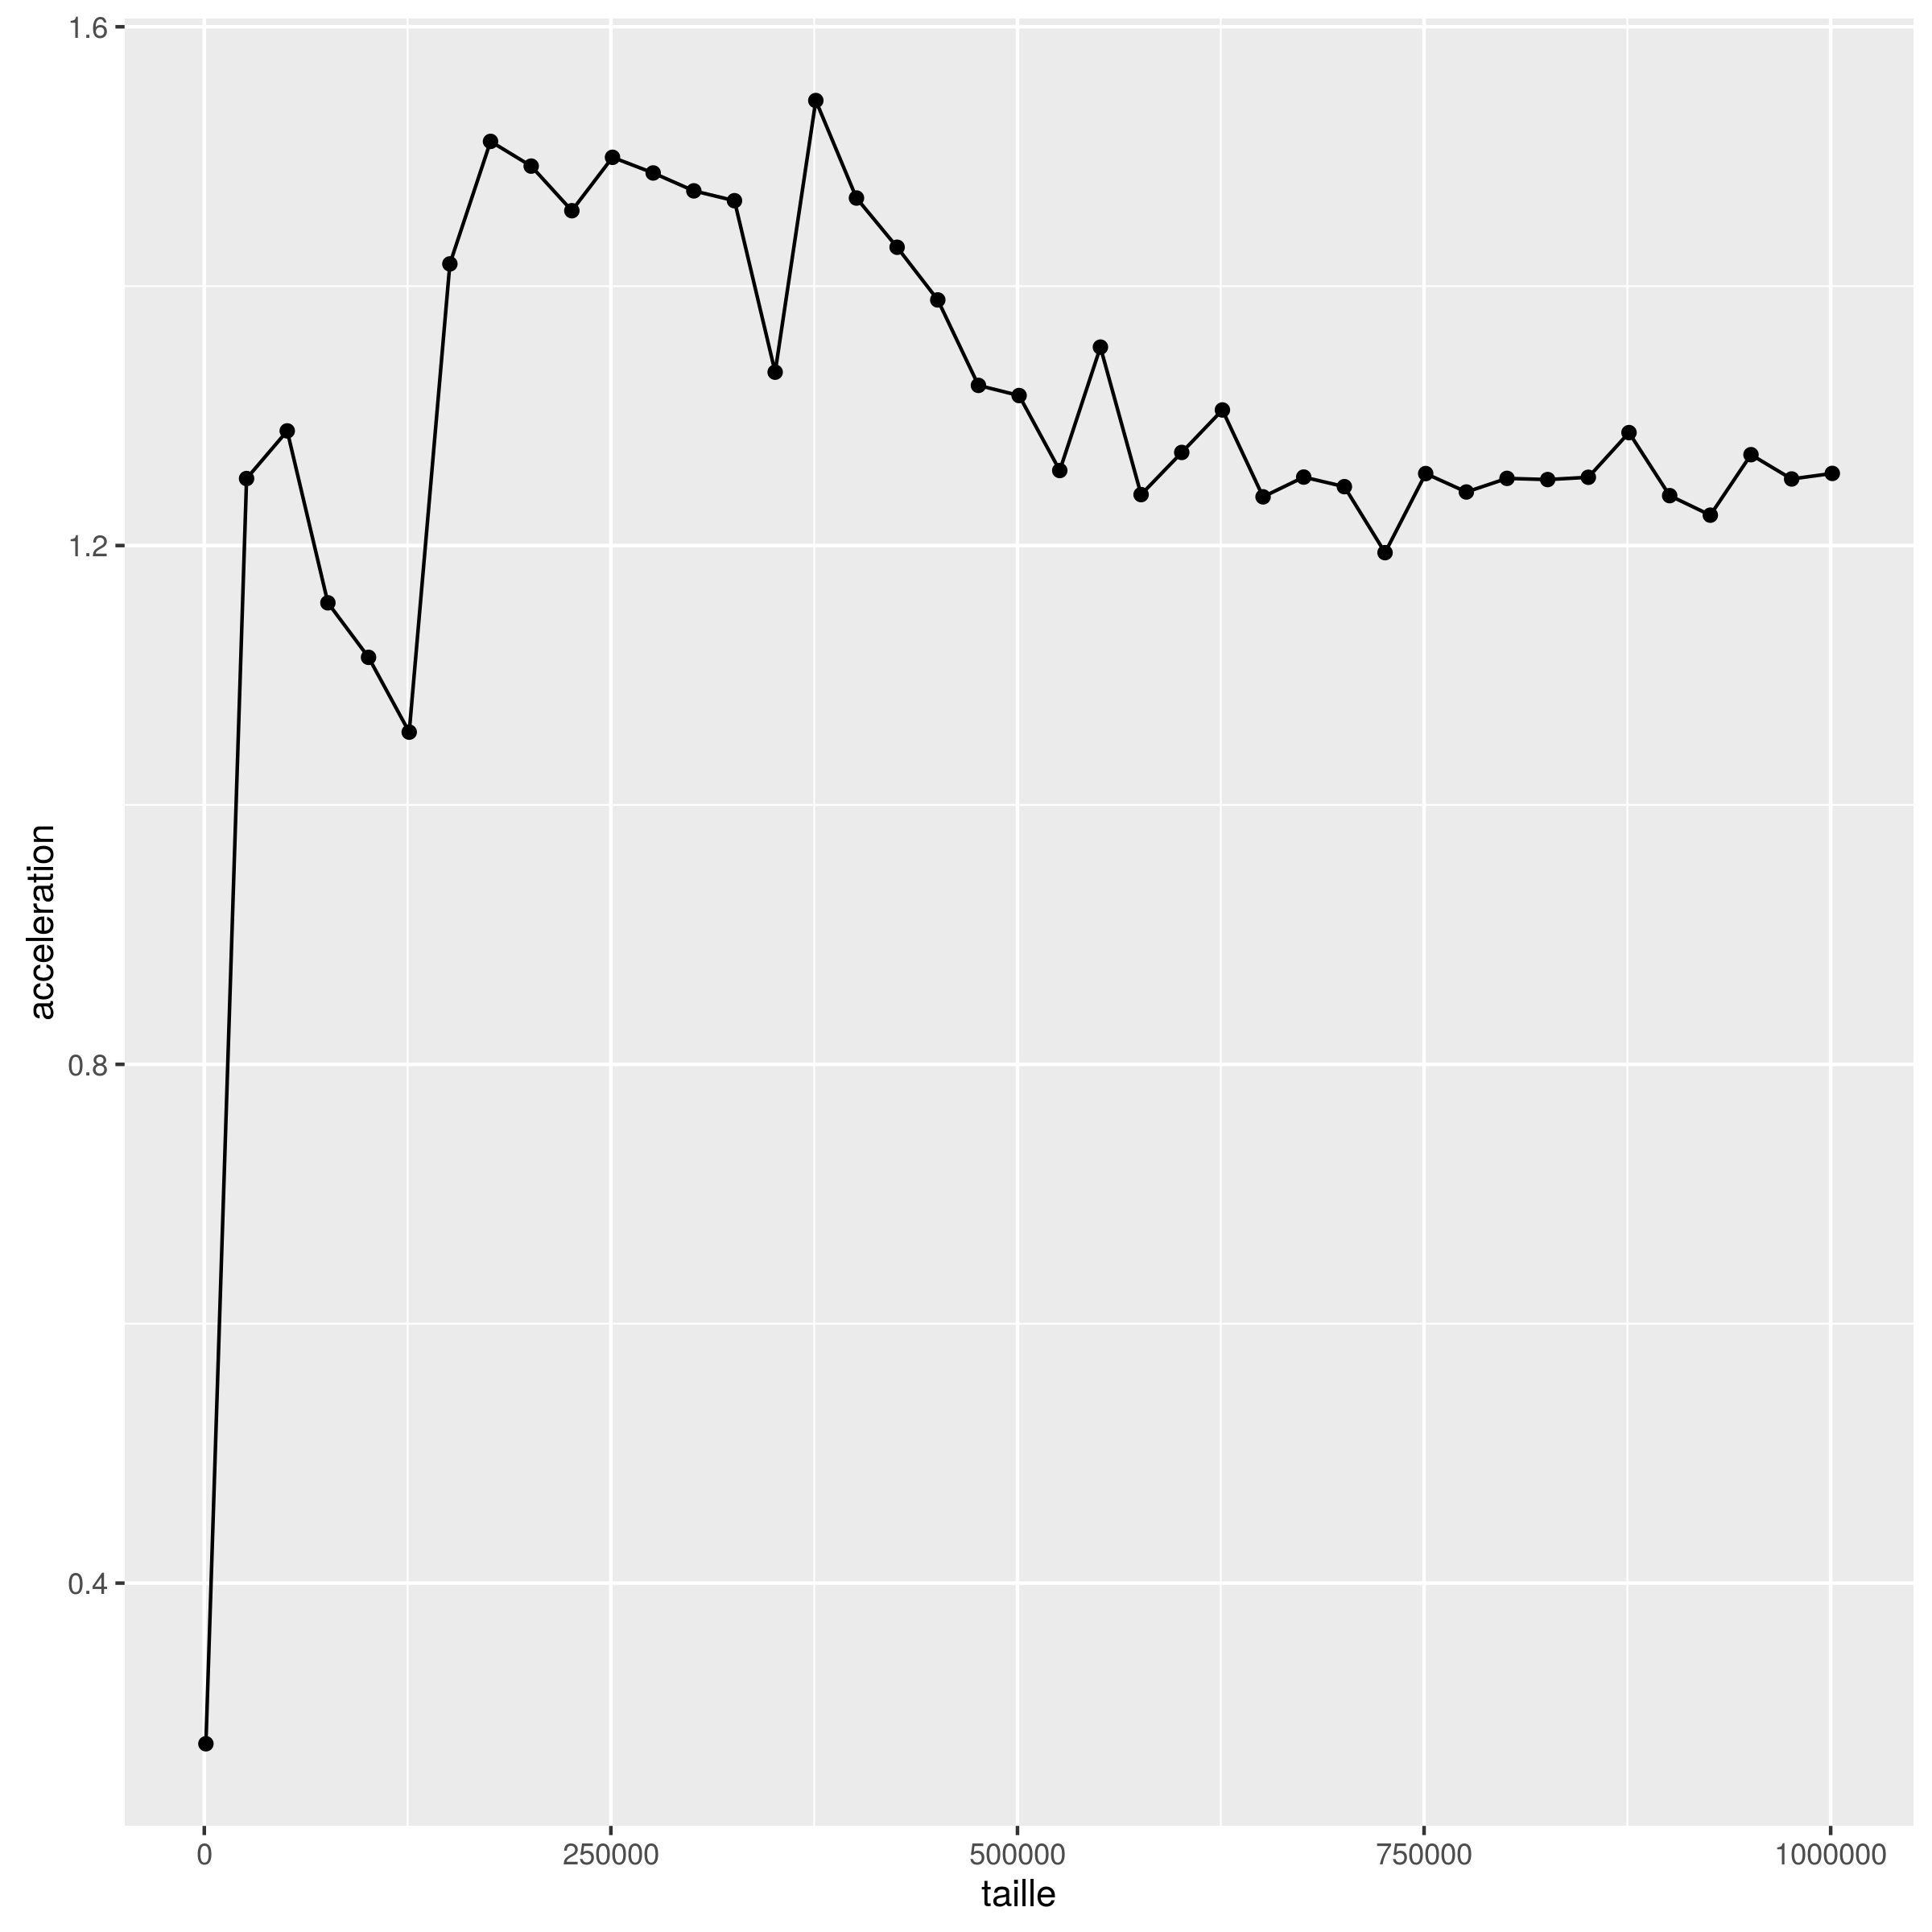
\includegraphics[scale=0.5] {graphes/global_temps_machine_accel11.png}
\end{figure}

Nous observons que pour des vecteurs allant d'une taille de 1000 \'el\'ements \`a 1000000 d'\'el\'ements, l'acc\'el\'eration est toujours sup\'erieur \`a 1. Nous observons aussi que l'acc\'el\'eration est la plus grande, pour des vecteurs d'une taille d'environ 450000 \'el\'ements. Pass\'e ce seuil, le niveau de l'acc\'el\'eration baisse.


\subsection{Temps CPU cumul\'e de l'utilisateur}
\begin{figure}[H] \center
   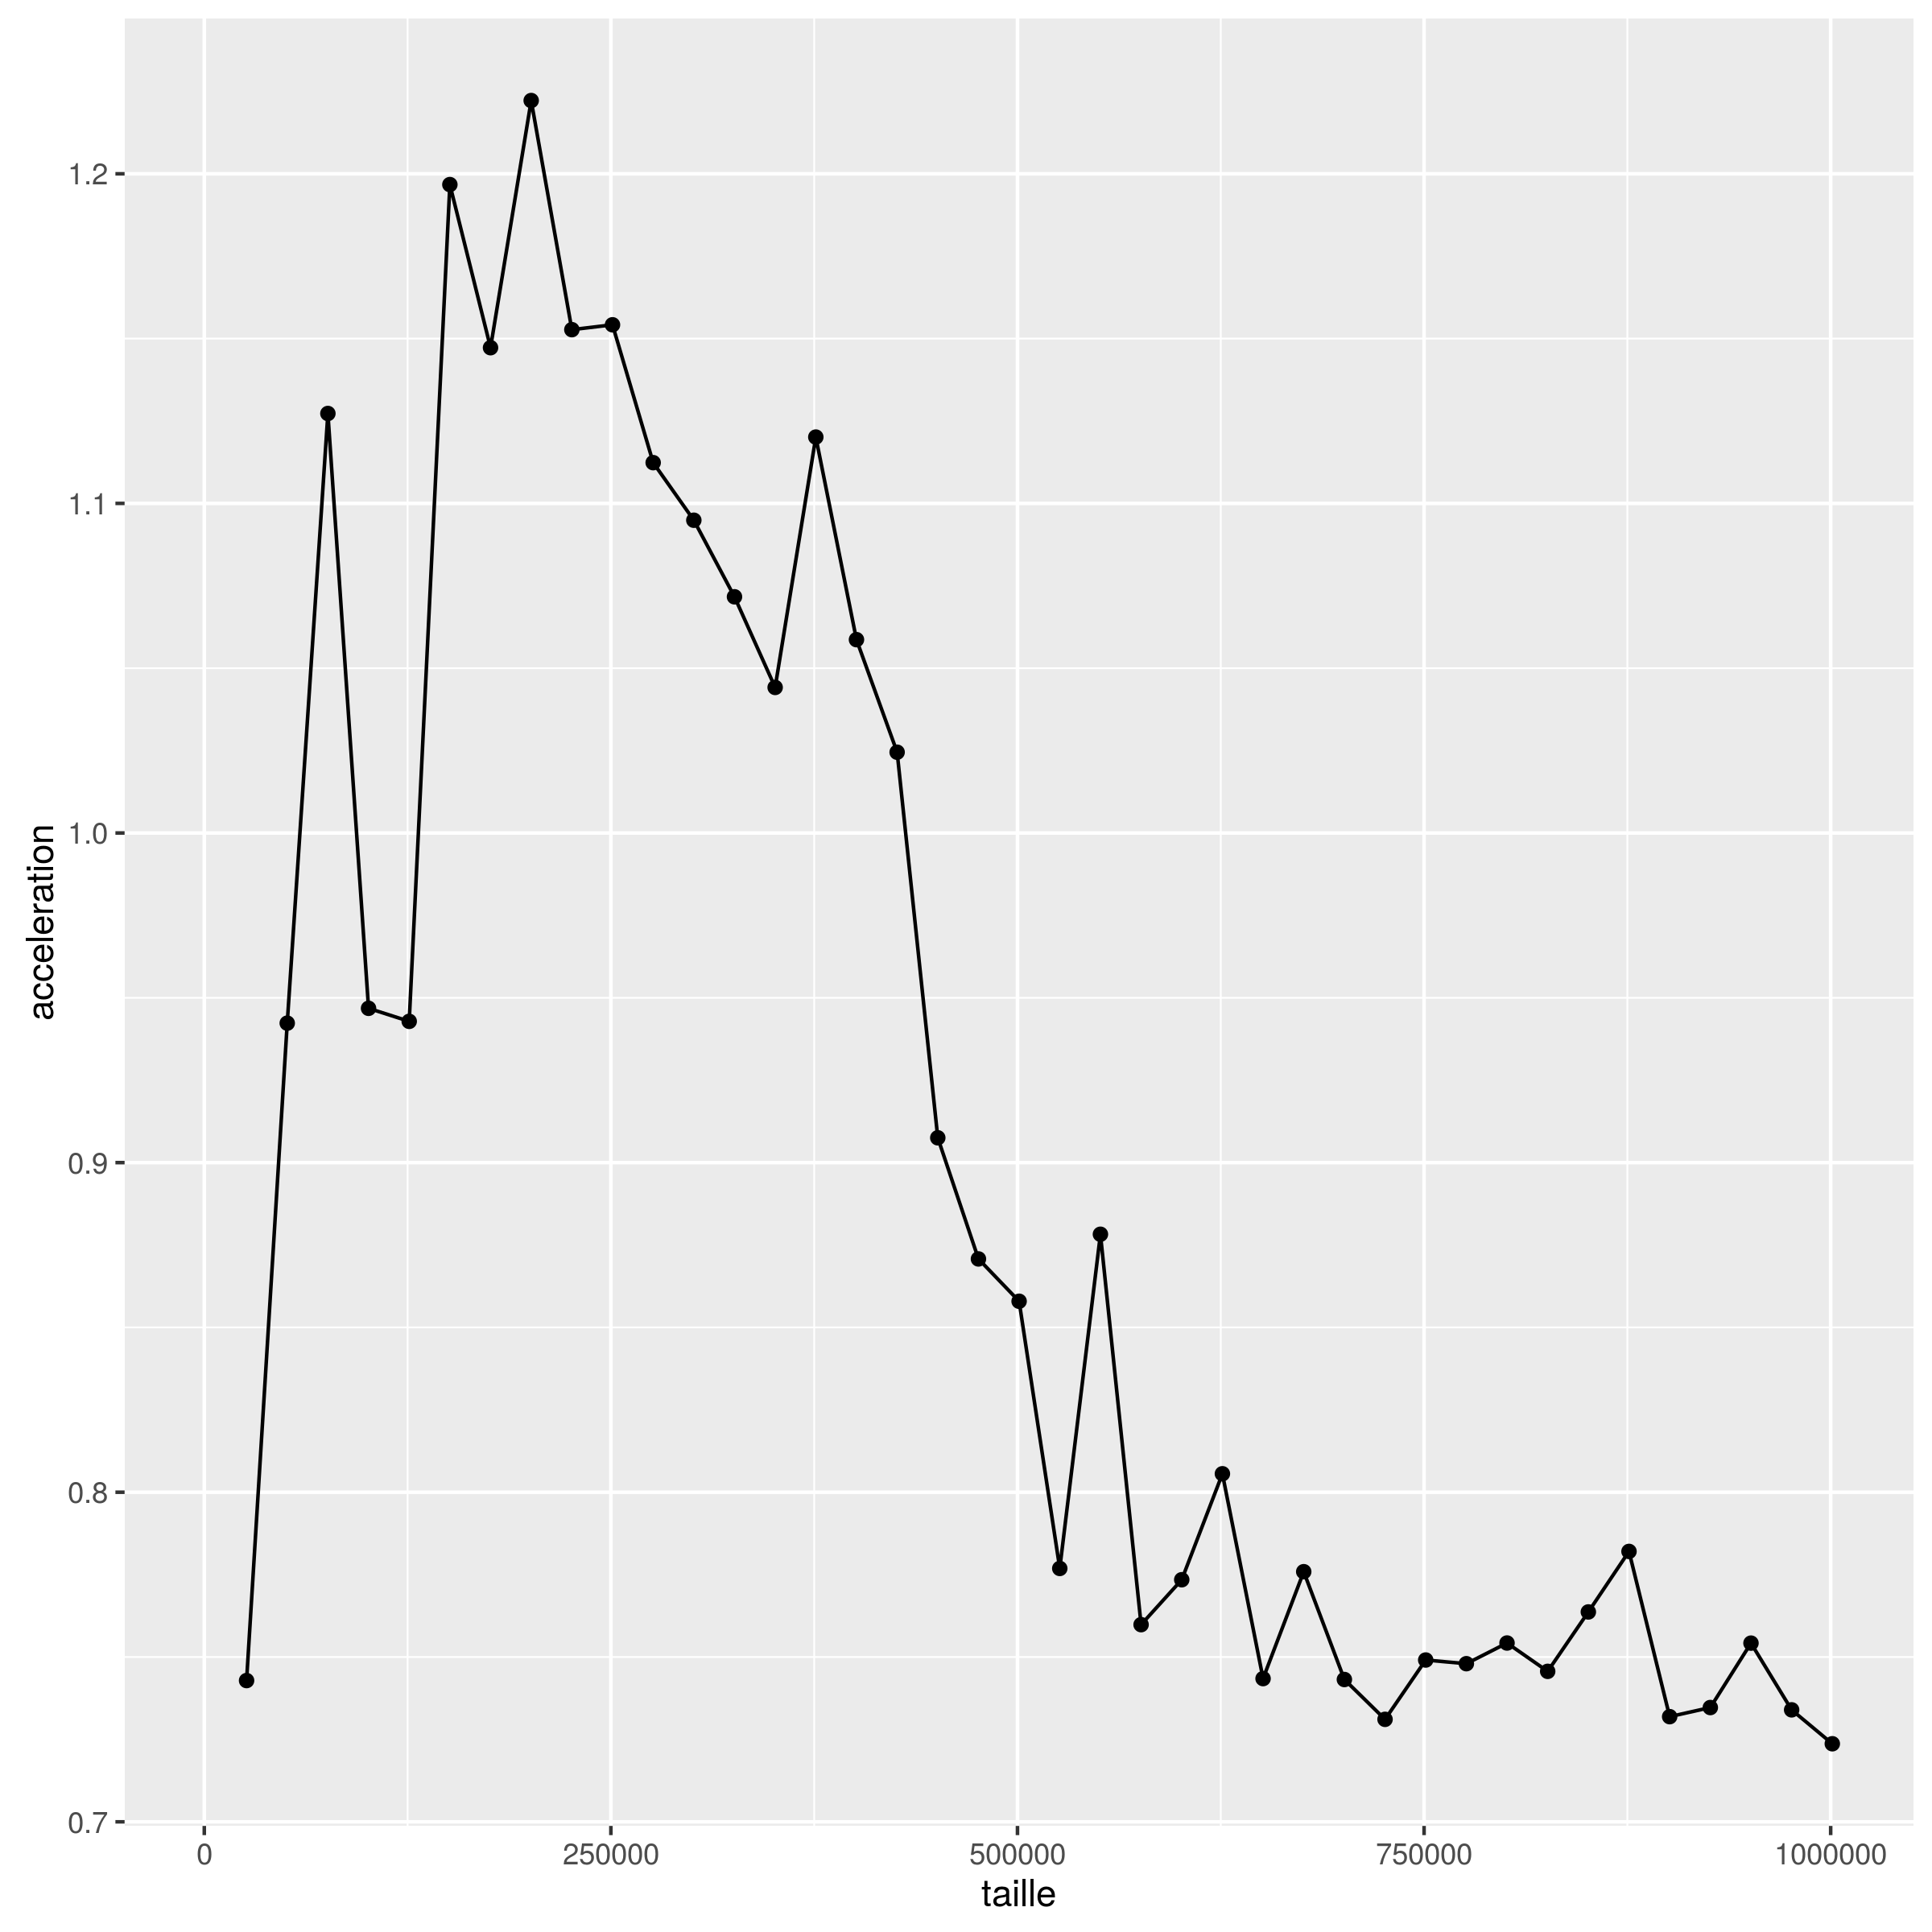
\includegraphics[scale=0.5] {graphes/temps_user_accel11.png}
\end{figure}
Nous observons que pour des vecteurs d'une taille inf\'erieur \`a 450000, l'acc\'el\'eration est sup\'erieur \`a 1. N\'eanmoins pass\'e ce seuil,  l'acc\'el\'eration est maintenant inf\'erieur \`a un, cela signifie que le temps CPU cumul\'e de l'utilisateur finit par \^{e}tre plus \'elev\'e avec 11 threads qu'en s\'equentiel. Cette acc\'el\'eration finit par tendre verss 0.7.


\section{Avec 12 threads}
\subsection{Temps d'ex\'ecution}

\begin{figure}[H] \center
   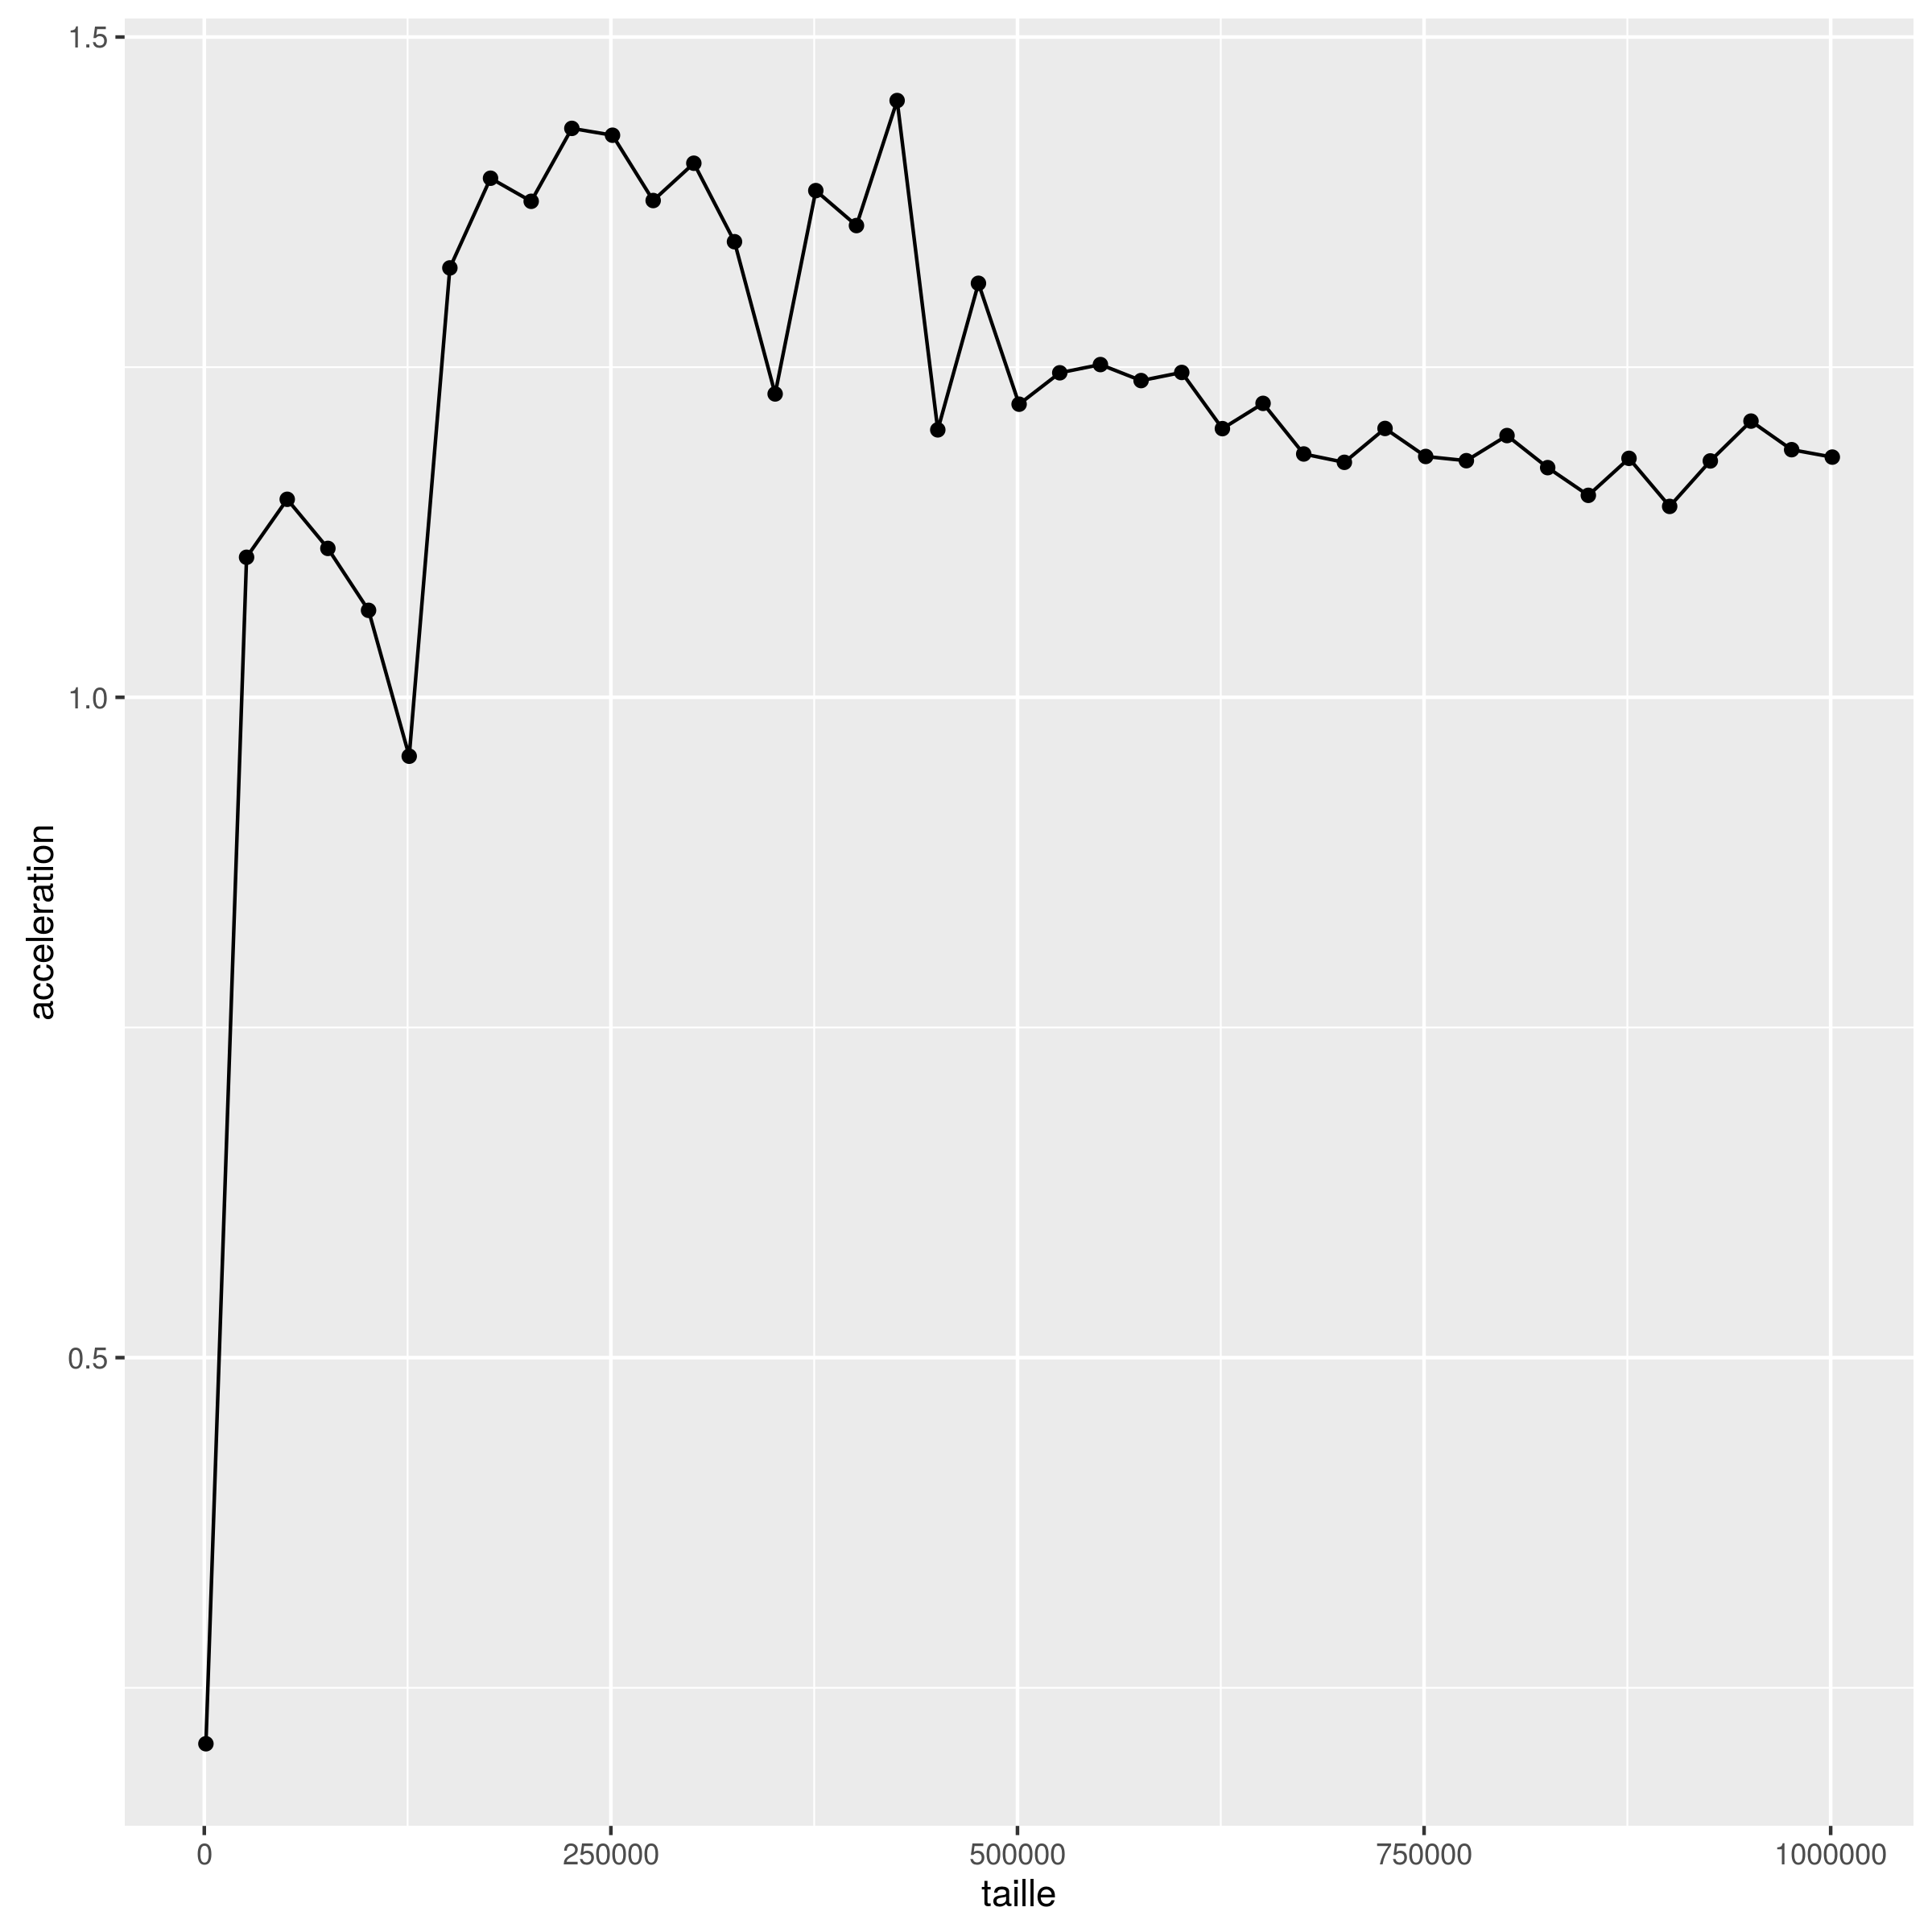
\includegraphics[scale=0.5] {graphes/global_temps_machine_accel12.png}
\end{figure}

Nous observons que pour des vecteurs allant d'une taille de 1000 \'el\'ements \`a 1000000 d'\'el\'ements, l'acc\'el\'eration est toujours sup\'erieur \`a 1. Nous observons aussi que l'acc\'el\'eration est la plus grande, pour des vecteurs d'une taille d'environ 400000 \'el\'ements. Pass\'e ce seuil, le niveau de l'acc\'el\'eration baisse et finit par tendre vers 1.2, pass\' le seuil des 500000 \'el\'ements.   


\subsection{Temps CPU cumul\'e de l'utilisateur}
\begin{figure}[H] \center
   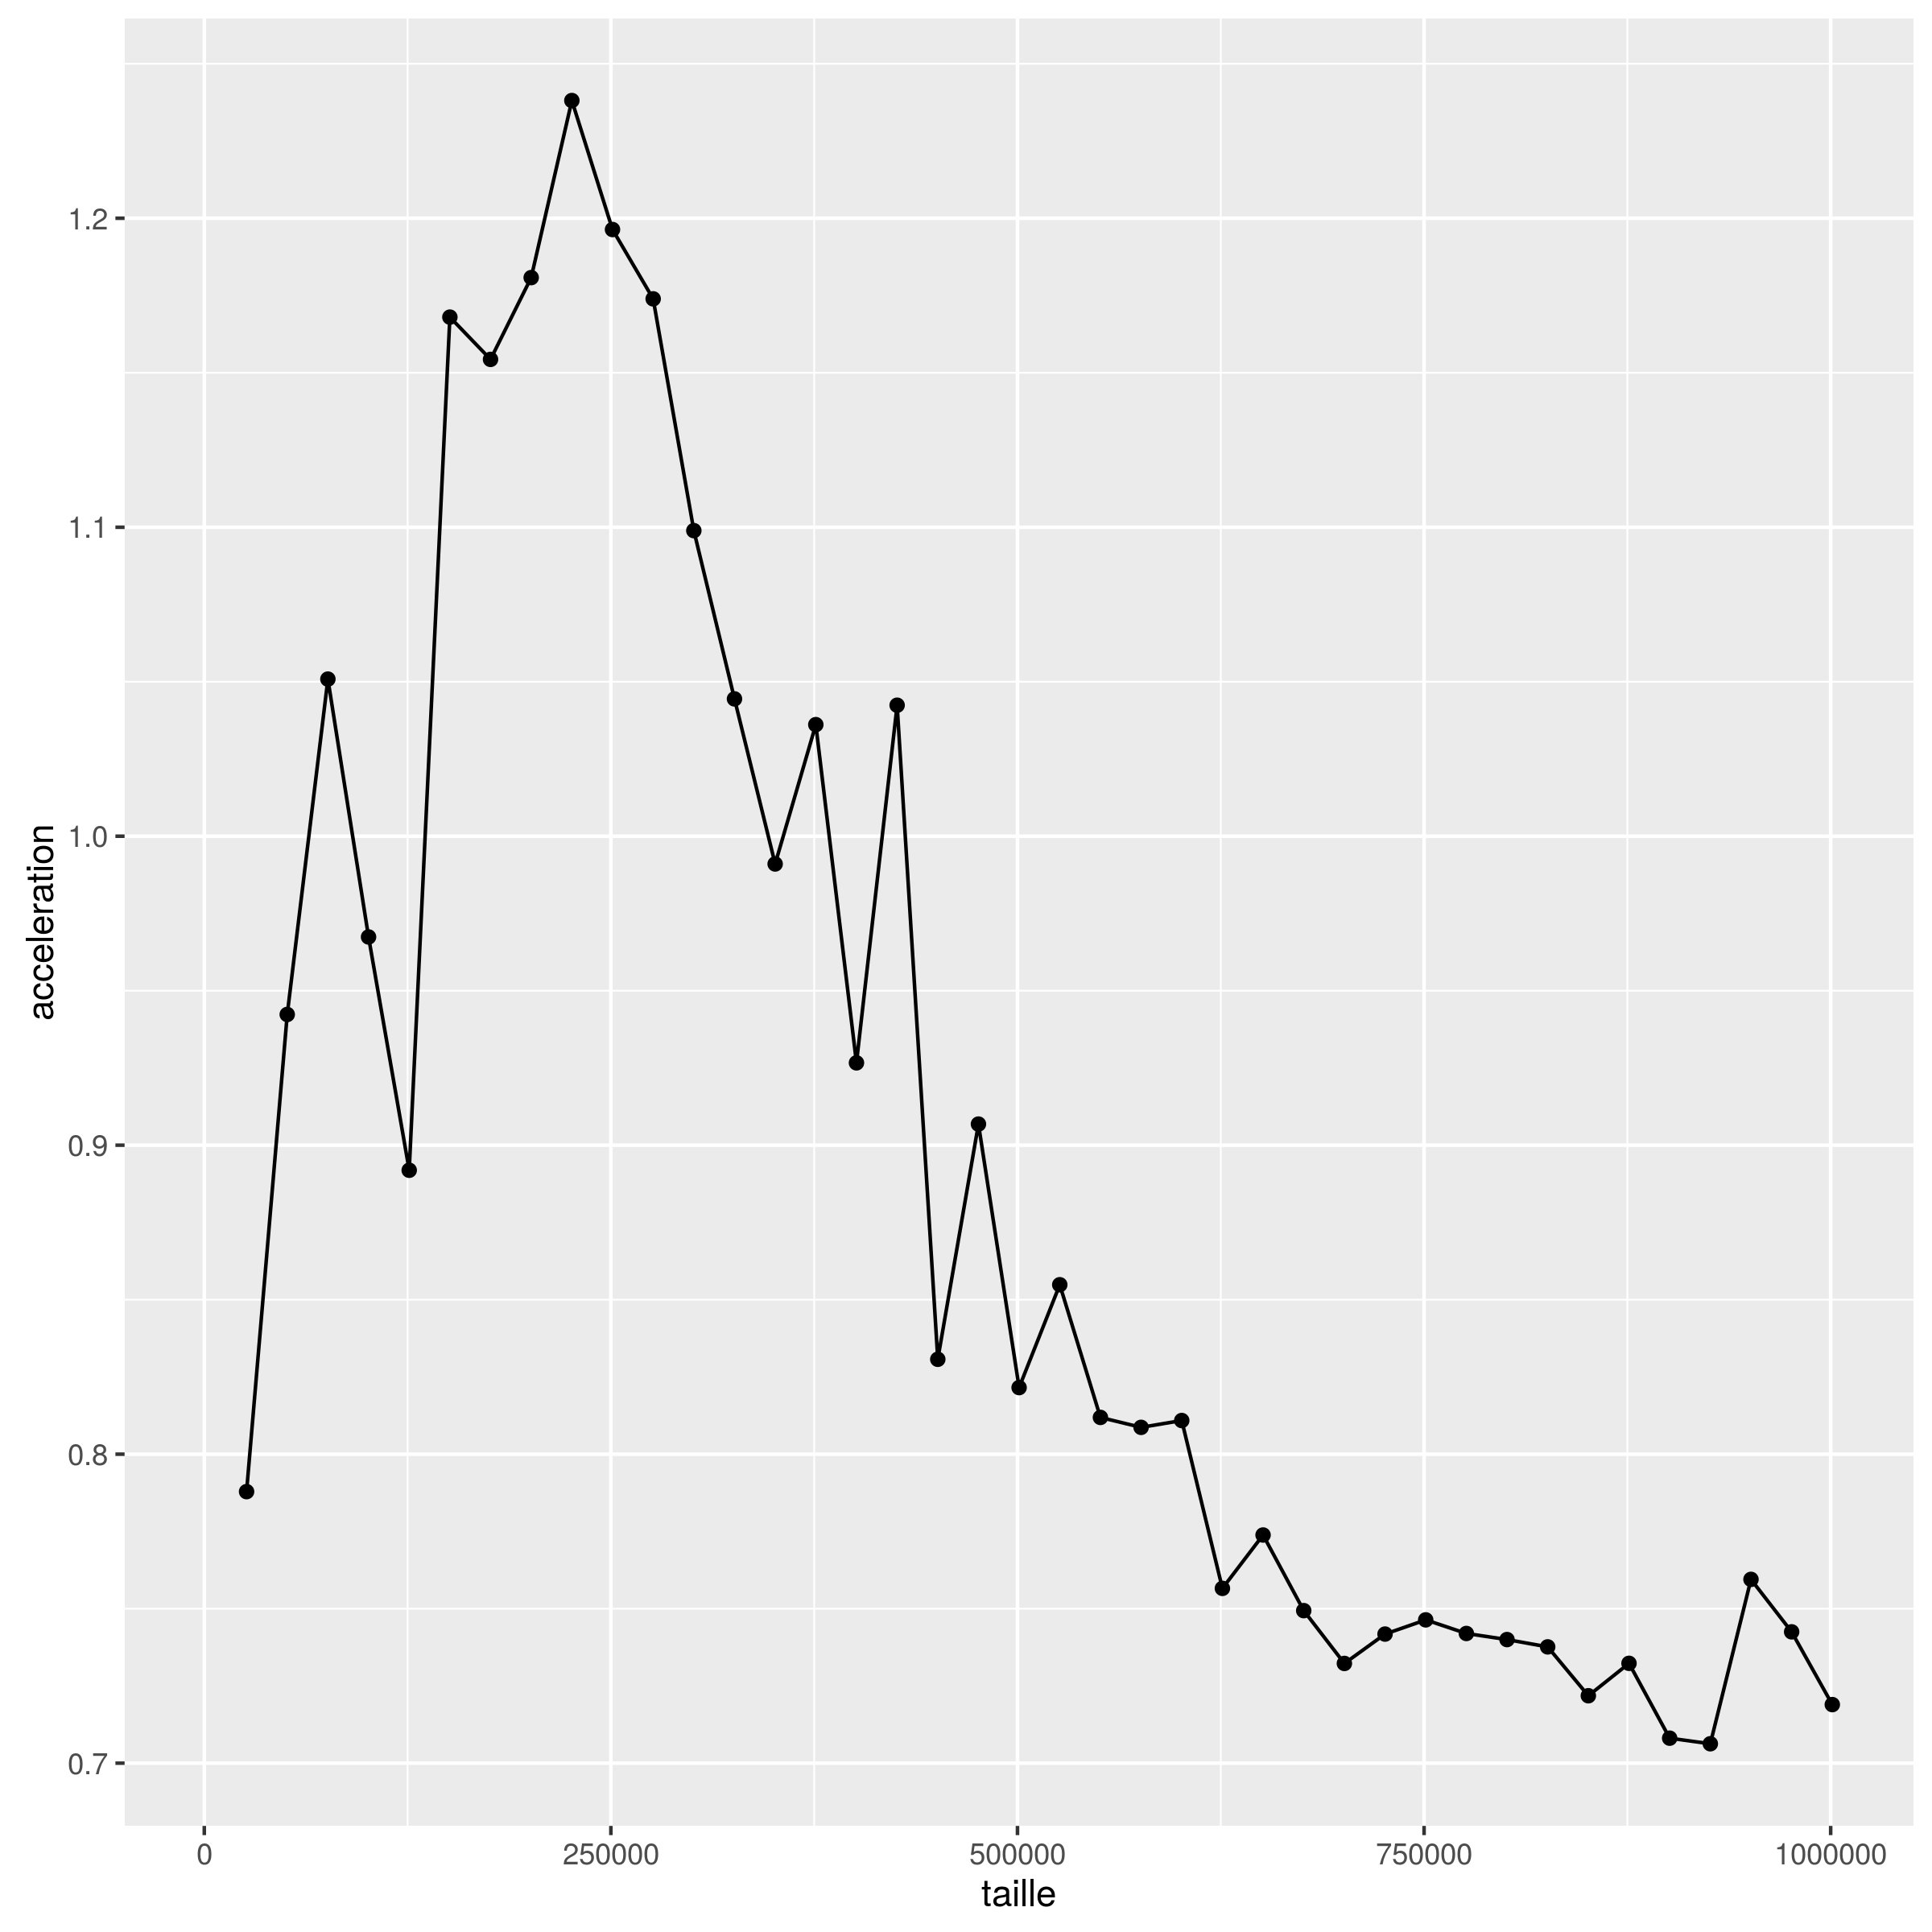
\includegraphics[scale=0.5] {graphes/temps_user_accel12.png}
\end{figure}
Nous observons que pour des vecteurs d'une taille inf\'erieur \`a 450000 et sup\'erieur \`a 25000, l'acc\'el\'eration est sup\'erieur \`a 1. N\'eanmoins pass\'e ce seuil,  l'acc\'el\'eration est maintenant inf\'erieur \`a un, cela signifie que le temps CPU cumul\'e de l'utilisateur finit par \^{e}tre plus \'elev\'e avec 12 threads qu'en s\'equentiel. Cette acc\'el\'eration finit par tendre vers 0.7.


\section{Avec 13 threads}
\subsection{Temps d'ex\'ecution}

\begin{figure}[H] \center
   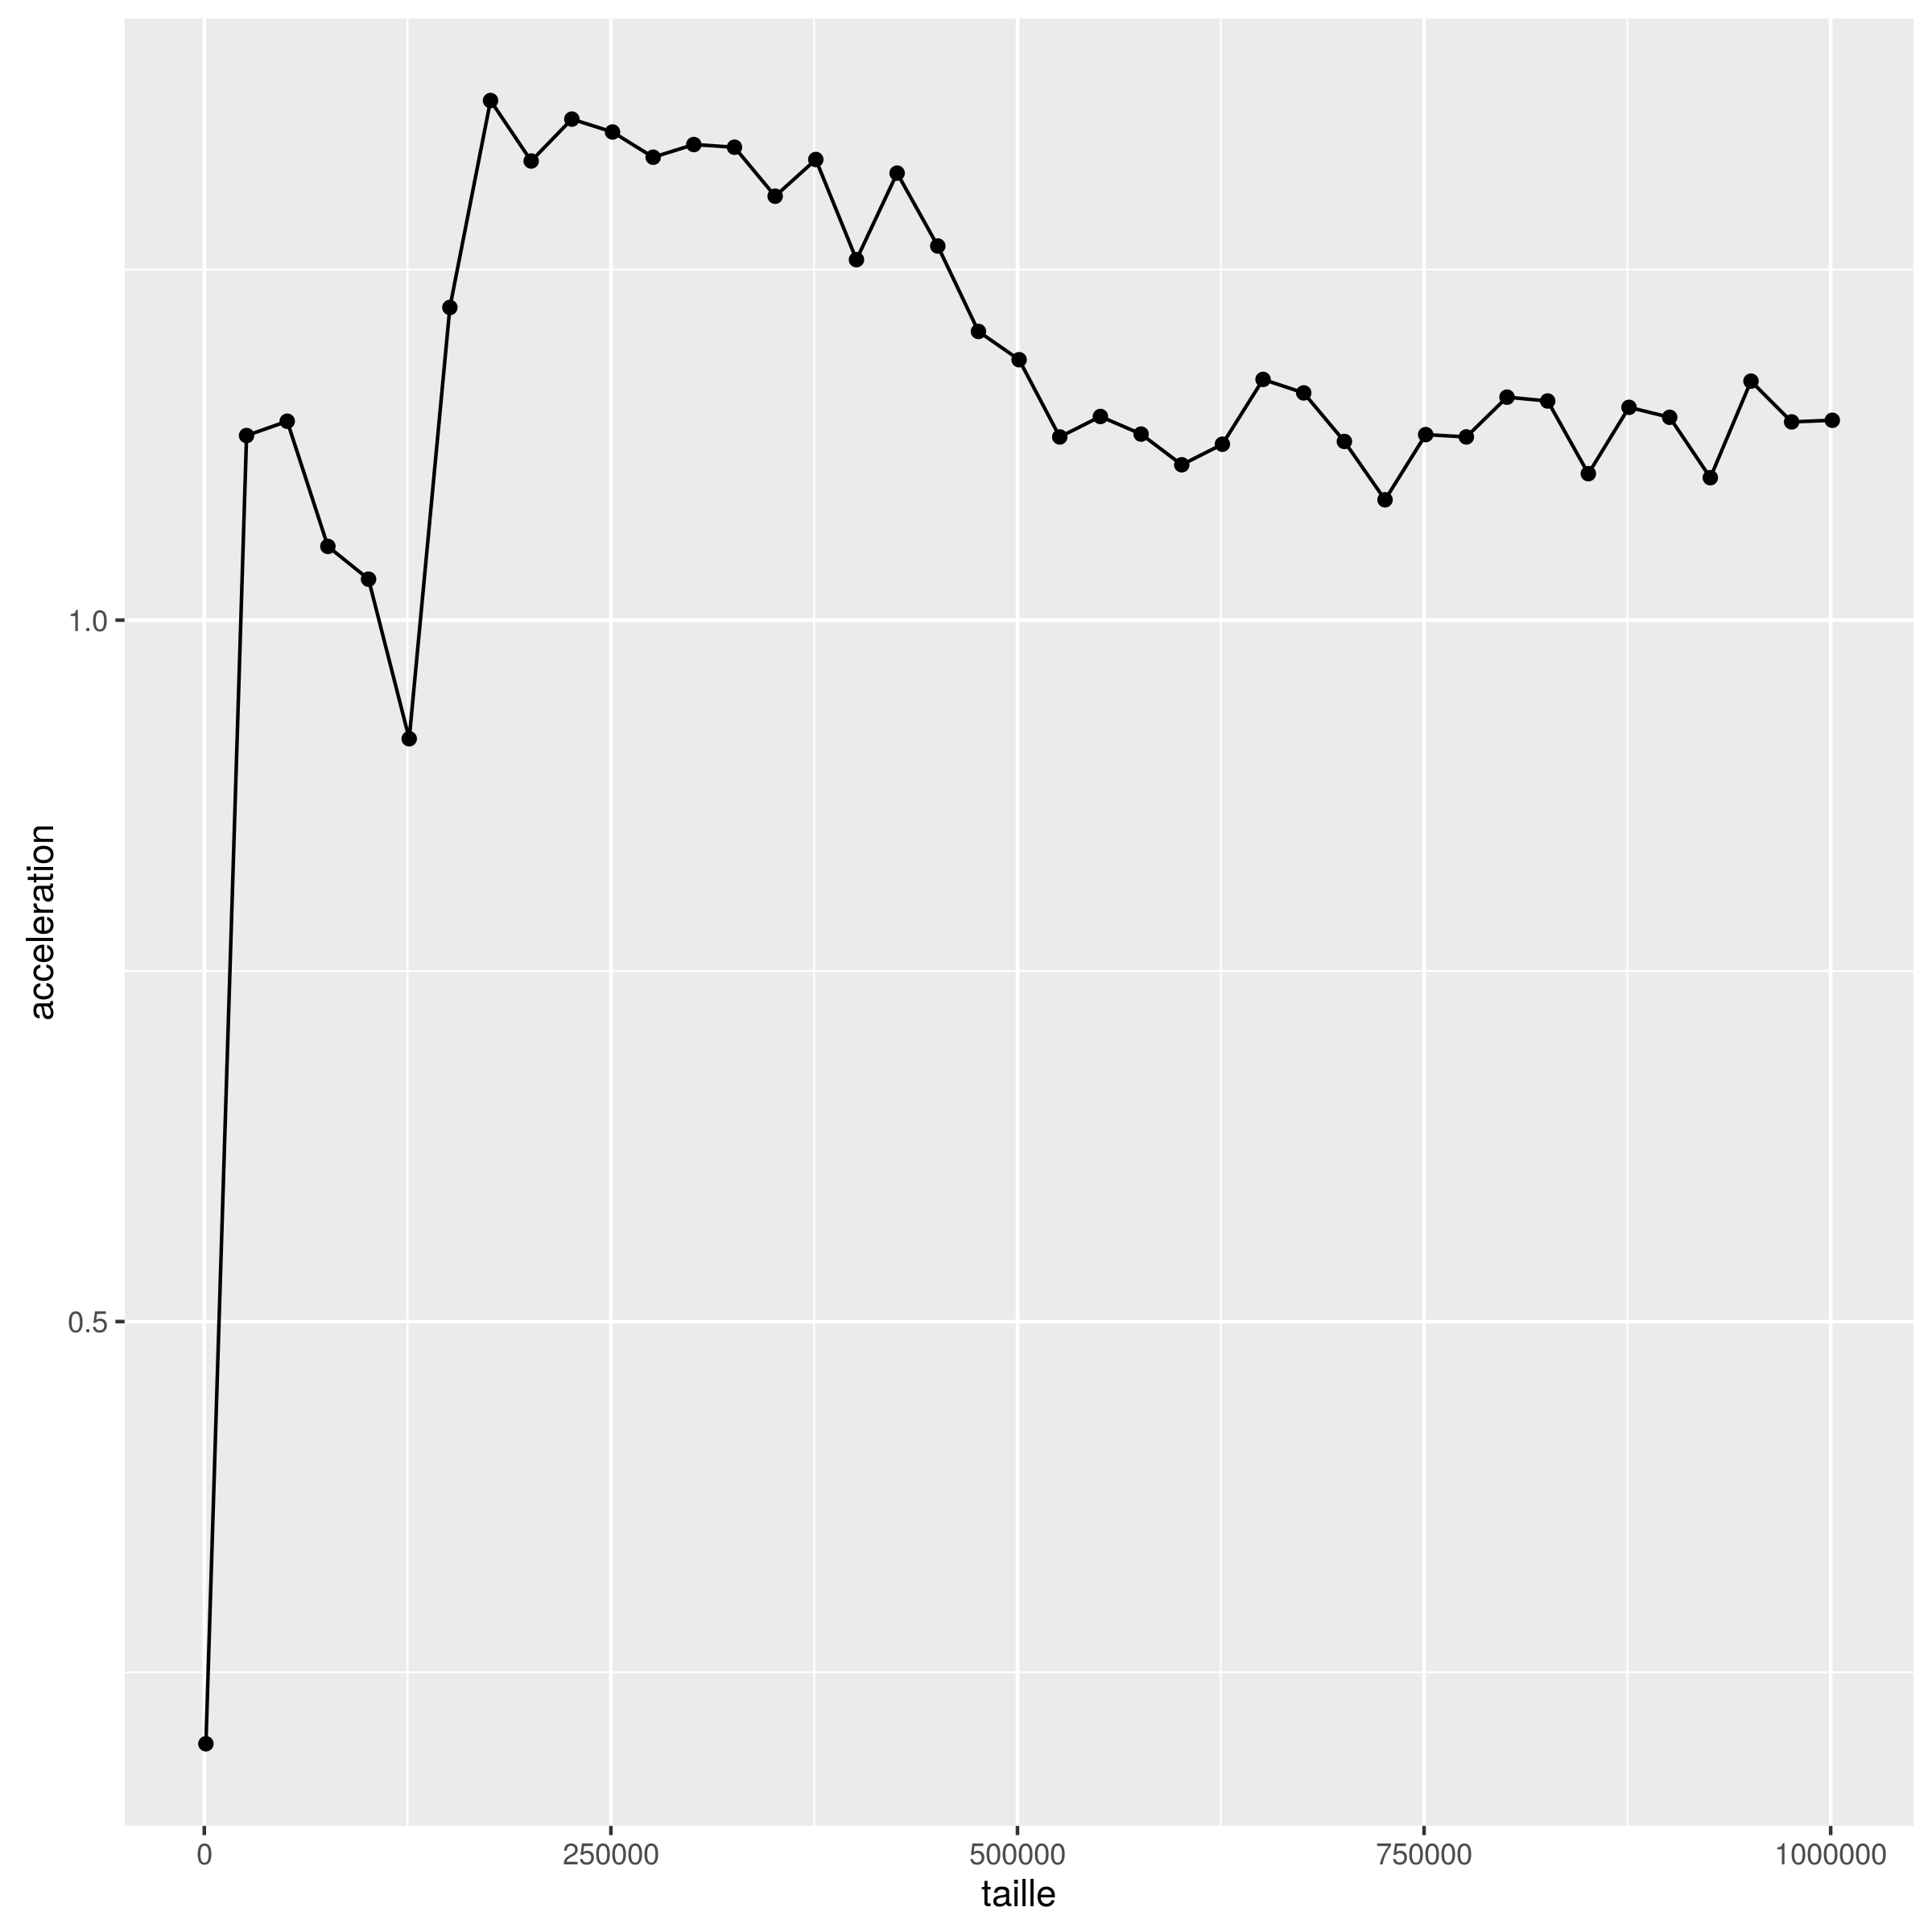
\includegraphics[scale=0.5] {graphes/global_temps_machine_accel13.png}
\end{figure}

Nous observons que pour des vecteurs allant d'une taille de 1000 \'el\'ements \`a 1000000 d'\'el\'ements, l'acc\'el\'eration est toujours sup\'erieur \`a 1. Nous observons aussi que l'acc\'el\'eration est la plus grande, pour des vecteurs d'une taille d'environ 400000 \'el\'ements. Pass\'e ce seuil, le niveau de l'acc\'el\'eration baisse et finit par tendre vers 1.2, pass\' le seuil des 500000 \'el\'ements.   


\subsection{Temps CPU cumul\'e de l'utilisateur}
\begin{figure}[H] \center
   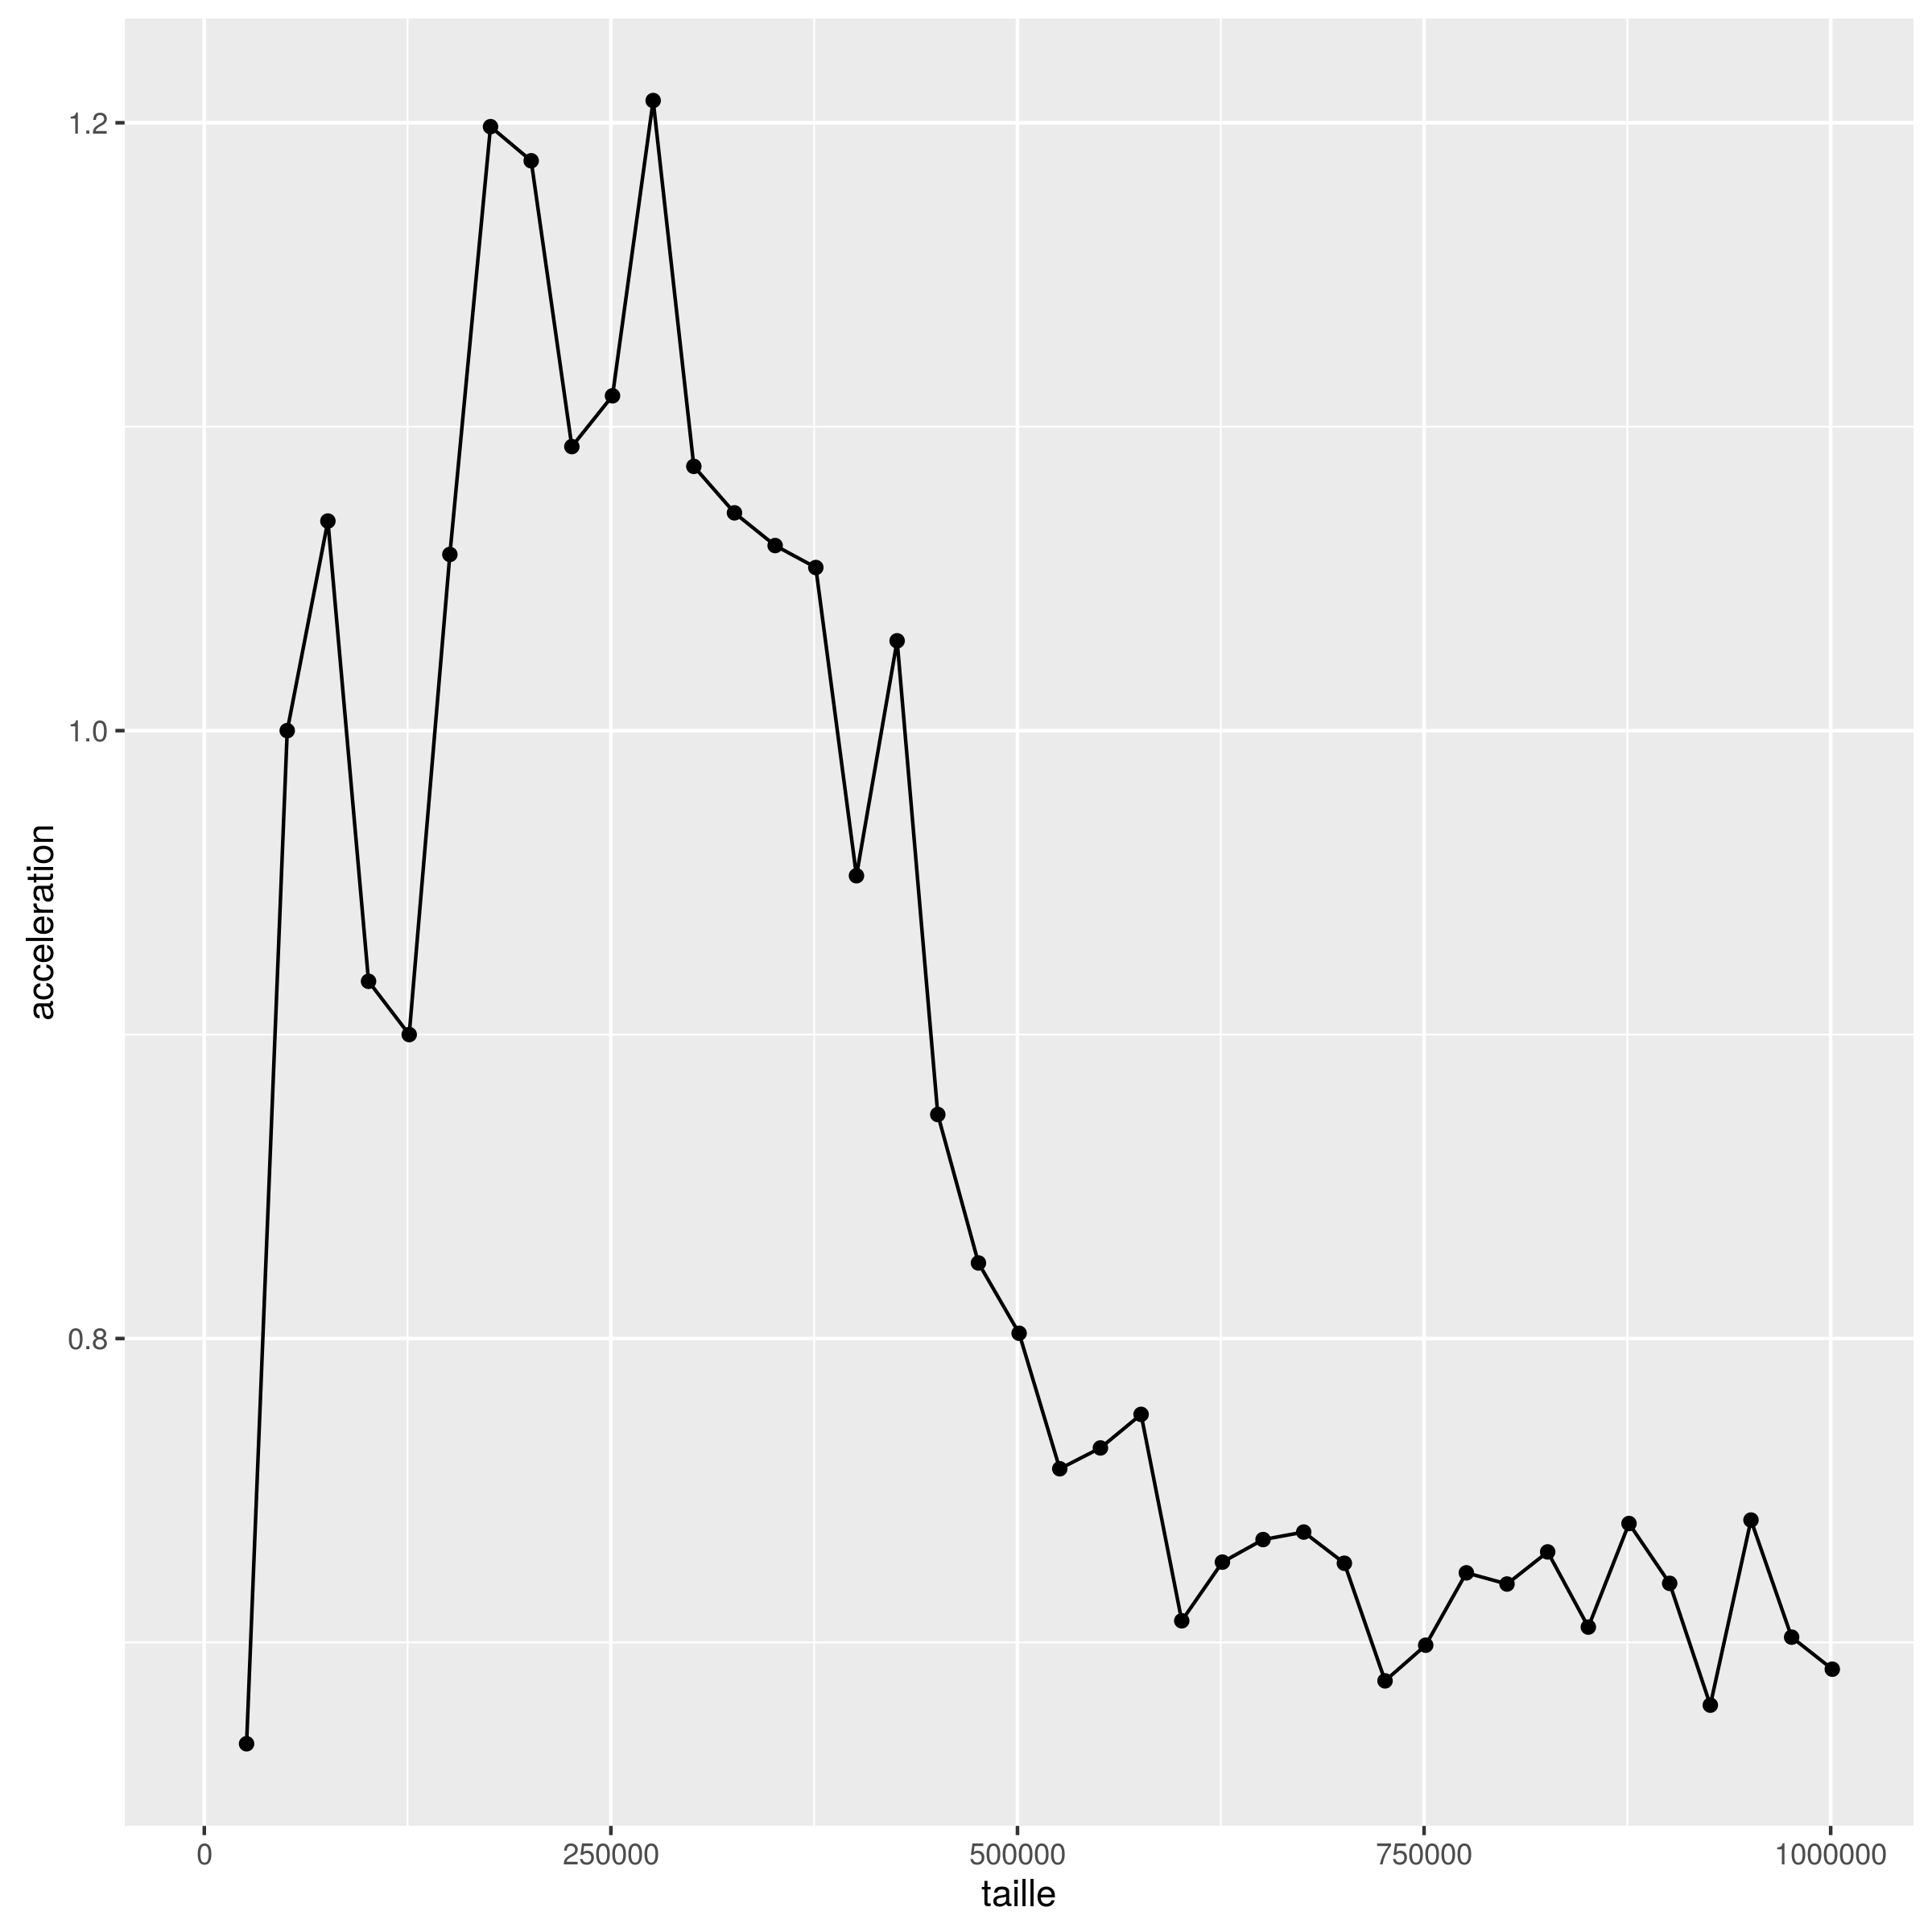
\includegraphics[scale=0.5] {graphes/temps_user_accel13.png}
\end{figure}
Nous observons que pour des vecteurs d'une taille inf\'erieur \`a 450000 et sup\'erieur \`a 25000, l'acc\'el\'eration est sup\'erieur \`a 1. N\'eanmoins pass\'e ce seuil,  l'acc\'el\'eration est maintenant inf\'erieur \`a un, cela signifie que le temps CPU cumul\'e de l'utilisateur finit par \^{e}tre plus \'elev\'e avec 13 threads qu'en s\'equentiel. Cette acc\'el\'eration finit par tendre vers 0.7.


\section{Avec 14 threads}
\subsection{Temps d'ex\'ecution}

\begin{figure}[H] \center
   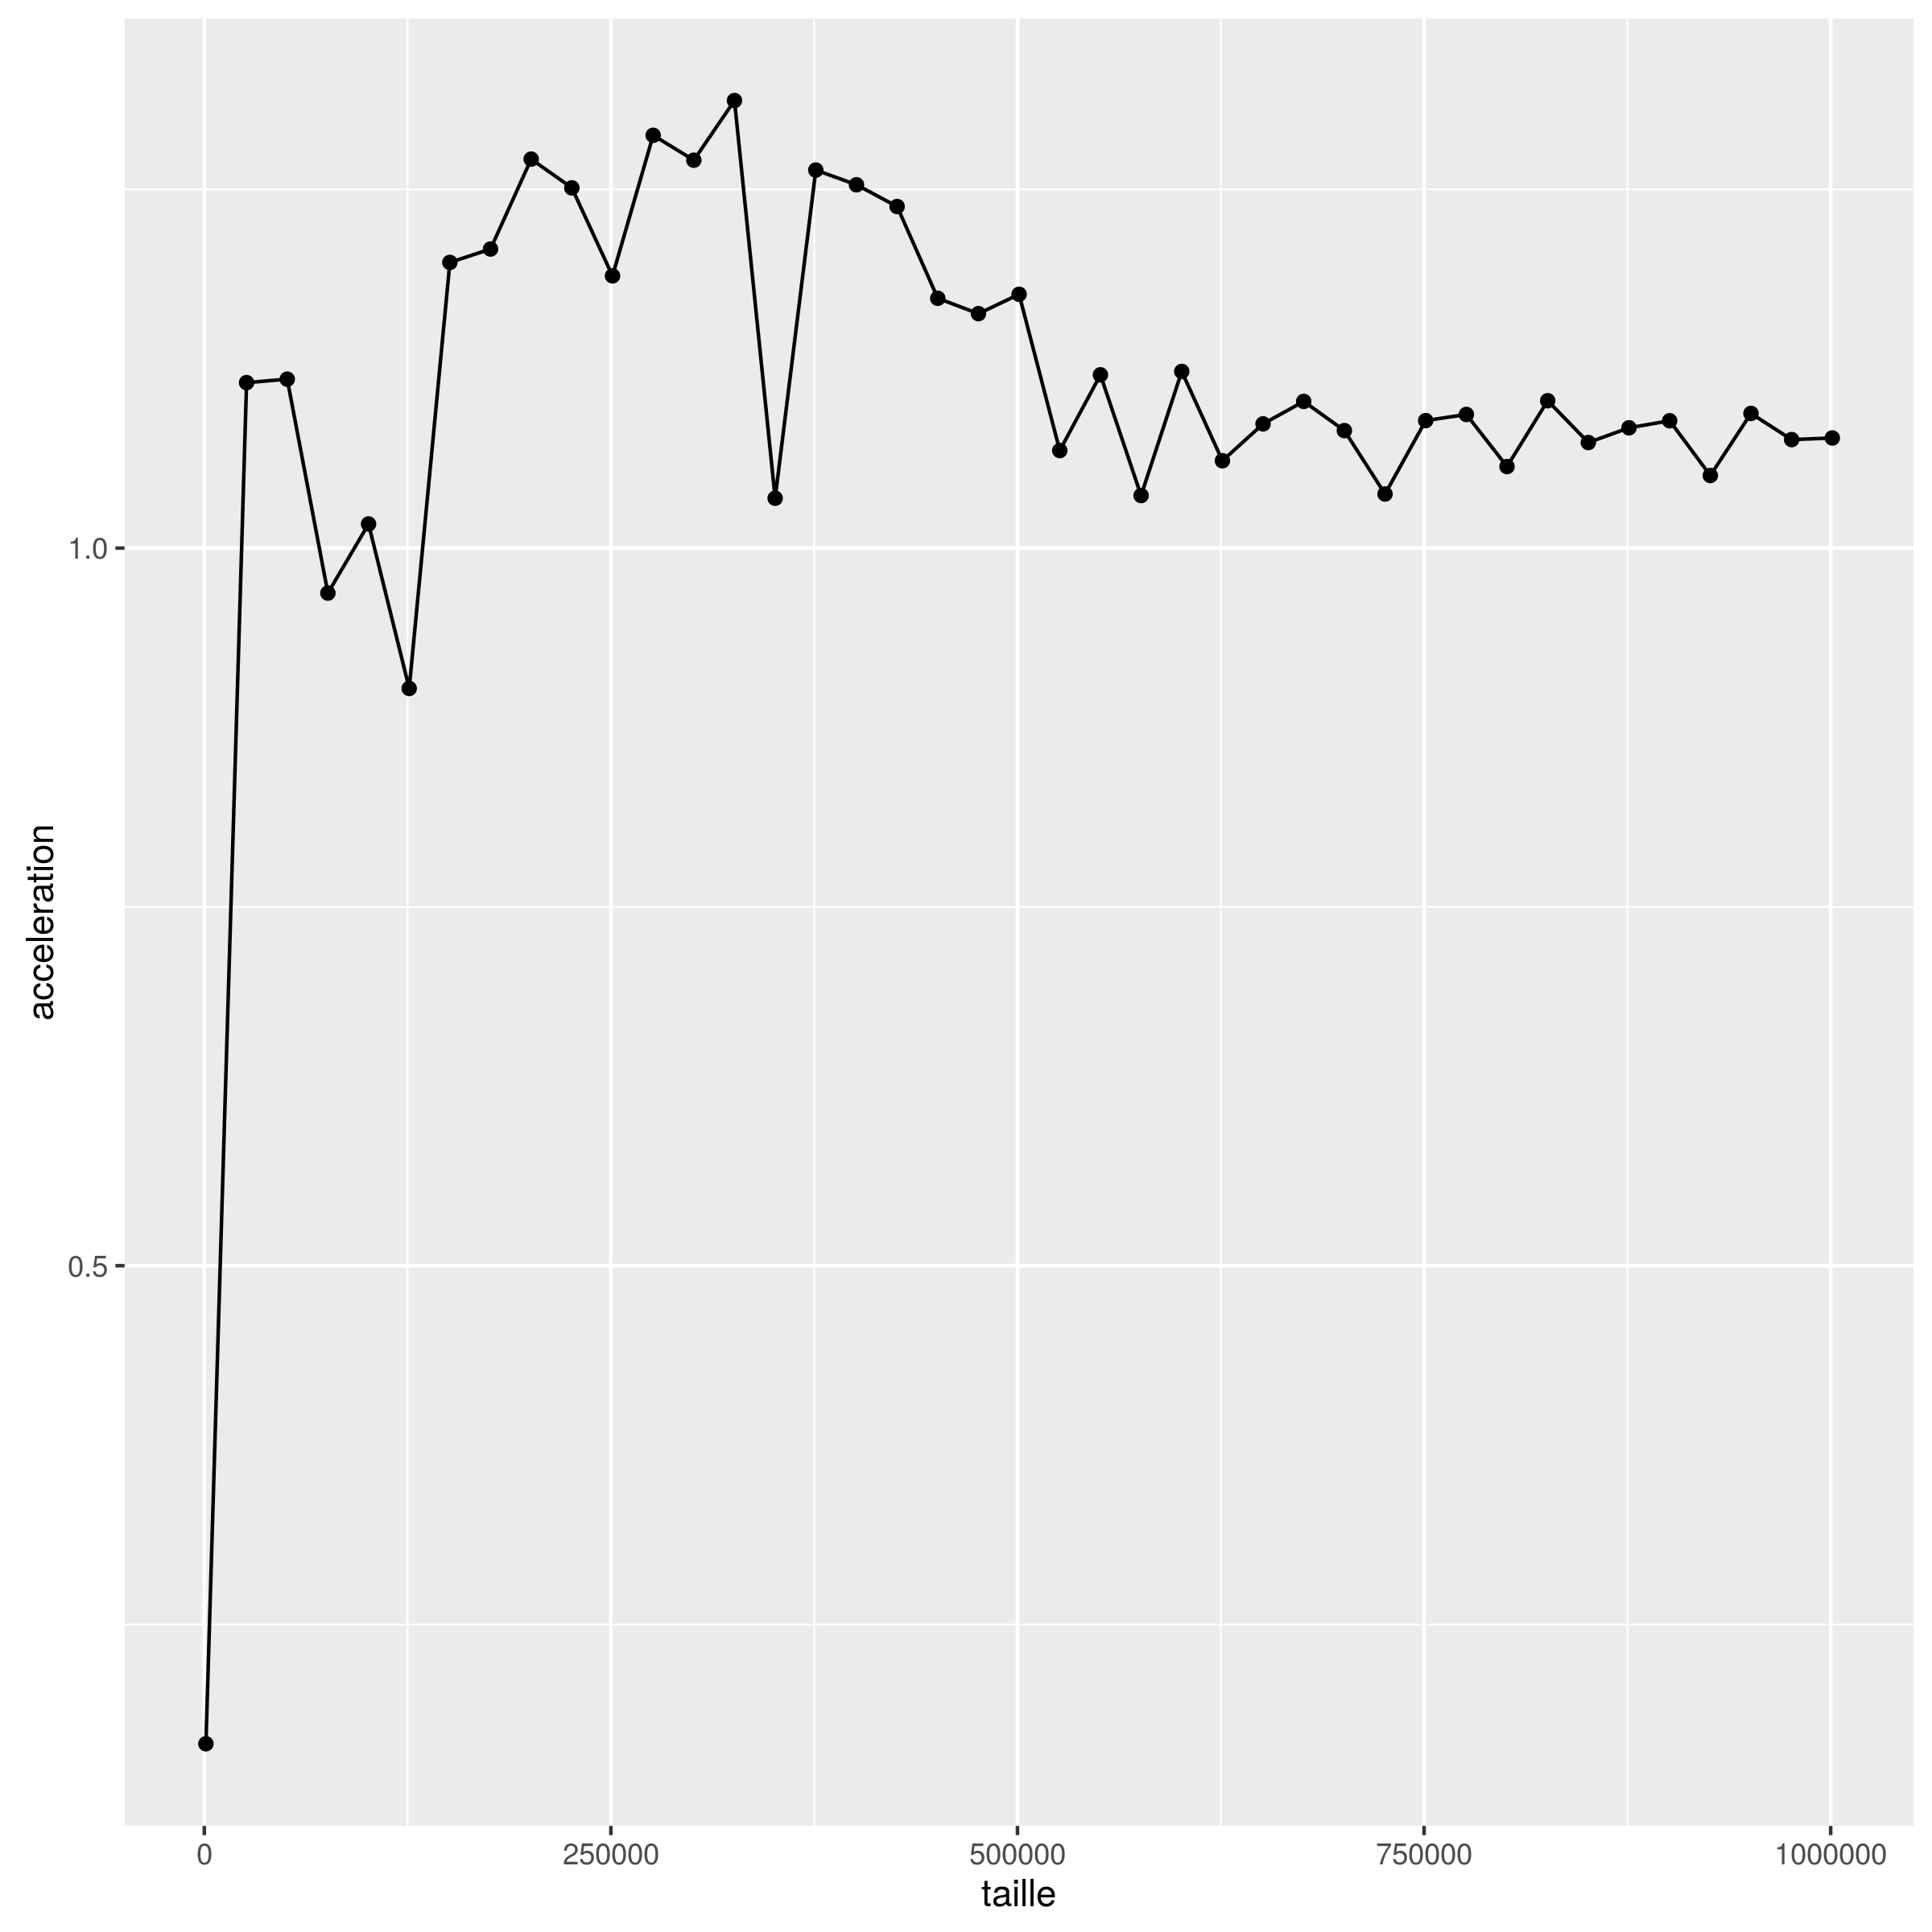
\includegraphics[scale=0.5] {graphes/global_temps_machine_accel14.png}
\end{figure}

Nous observons que pour des vecteurs allant d'une taille de 1000 \'el\'ements \`a 1000000 d'\'el\'ements, l'acc\'el\'eration est toujours sup\'erieur \`a 1. Nous observons aussi que l'acc\'el\'eration est la plus grande, pour des vecteurs d'une taille d'environ 400000 \'el\'ements. Pass\'e ce seuil, le niveau de l'acc\'el\'eration baisse et finit par tendre vers 1.2, pass\' le seuil des 500000 \'el\'ements.   


\subsection{Temps CPU cumul\'e de l'utilisateur}
\begin{figure}[H] \center
   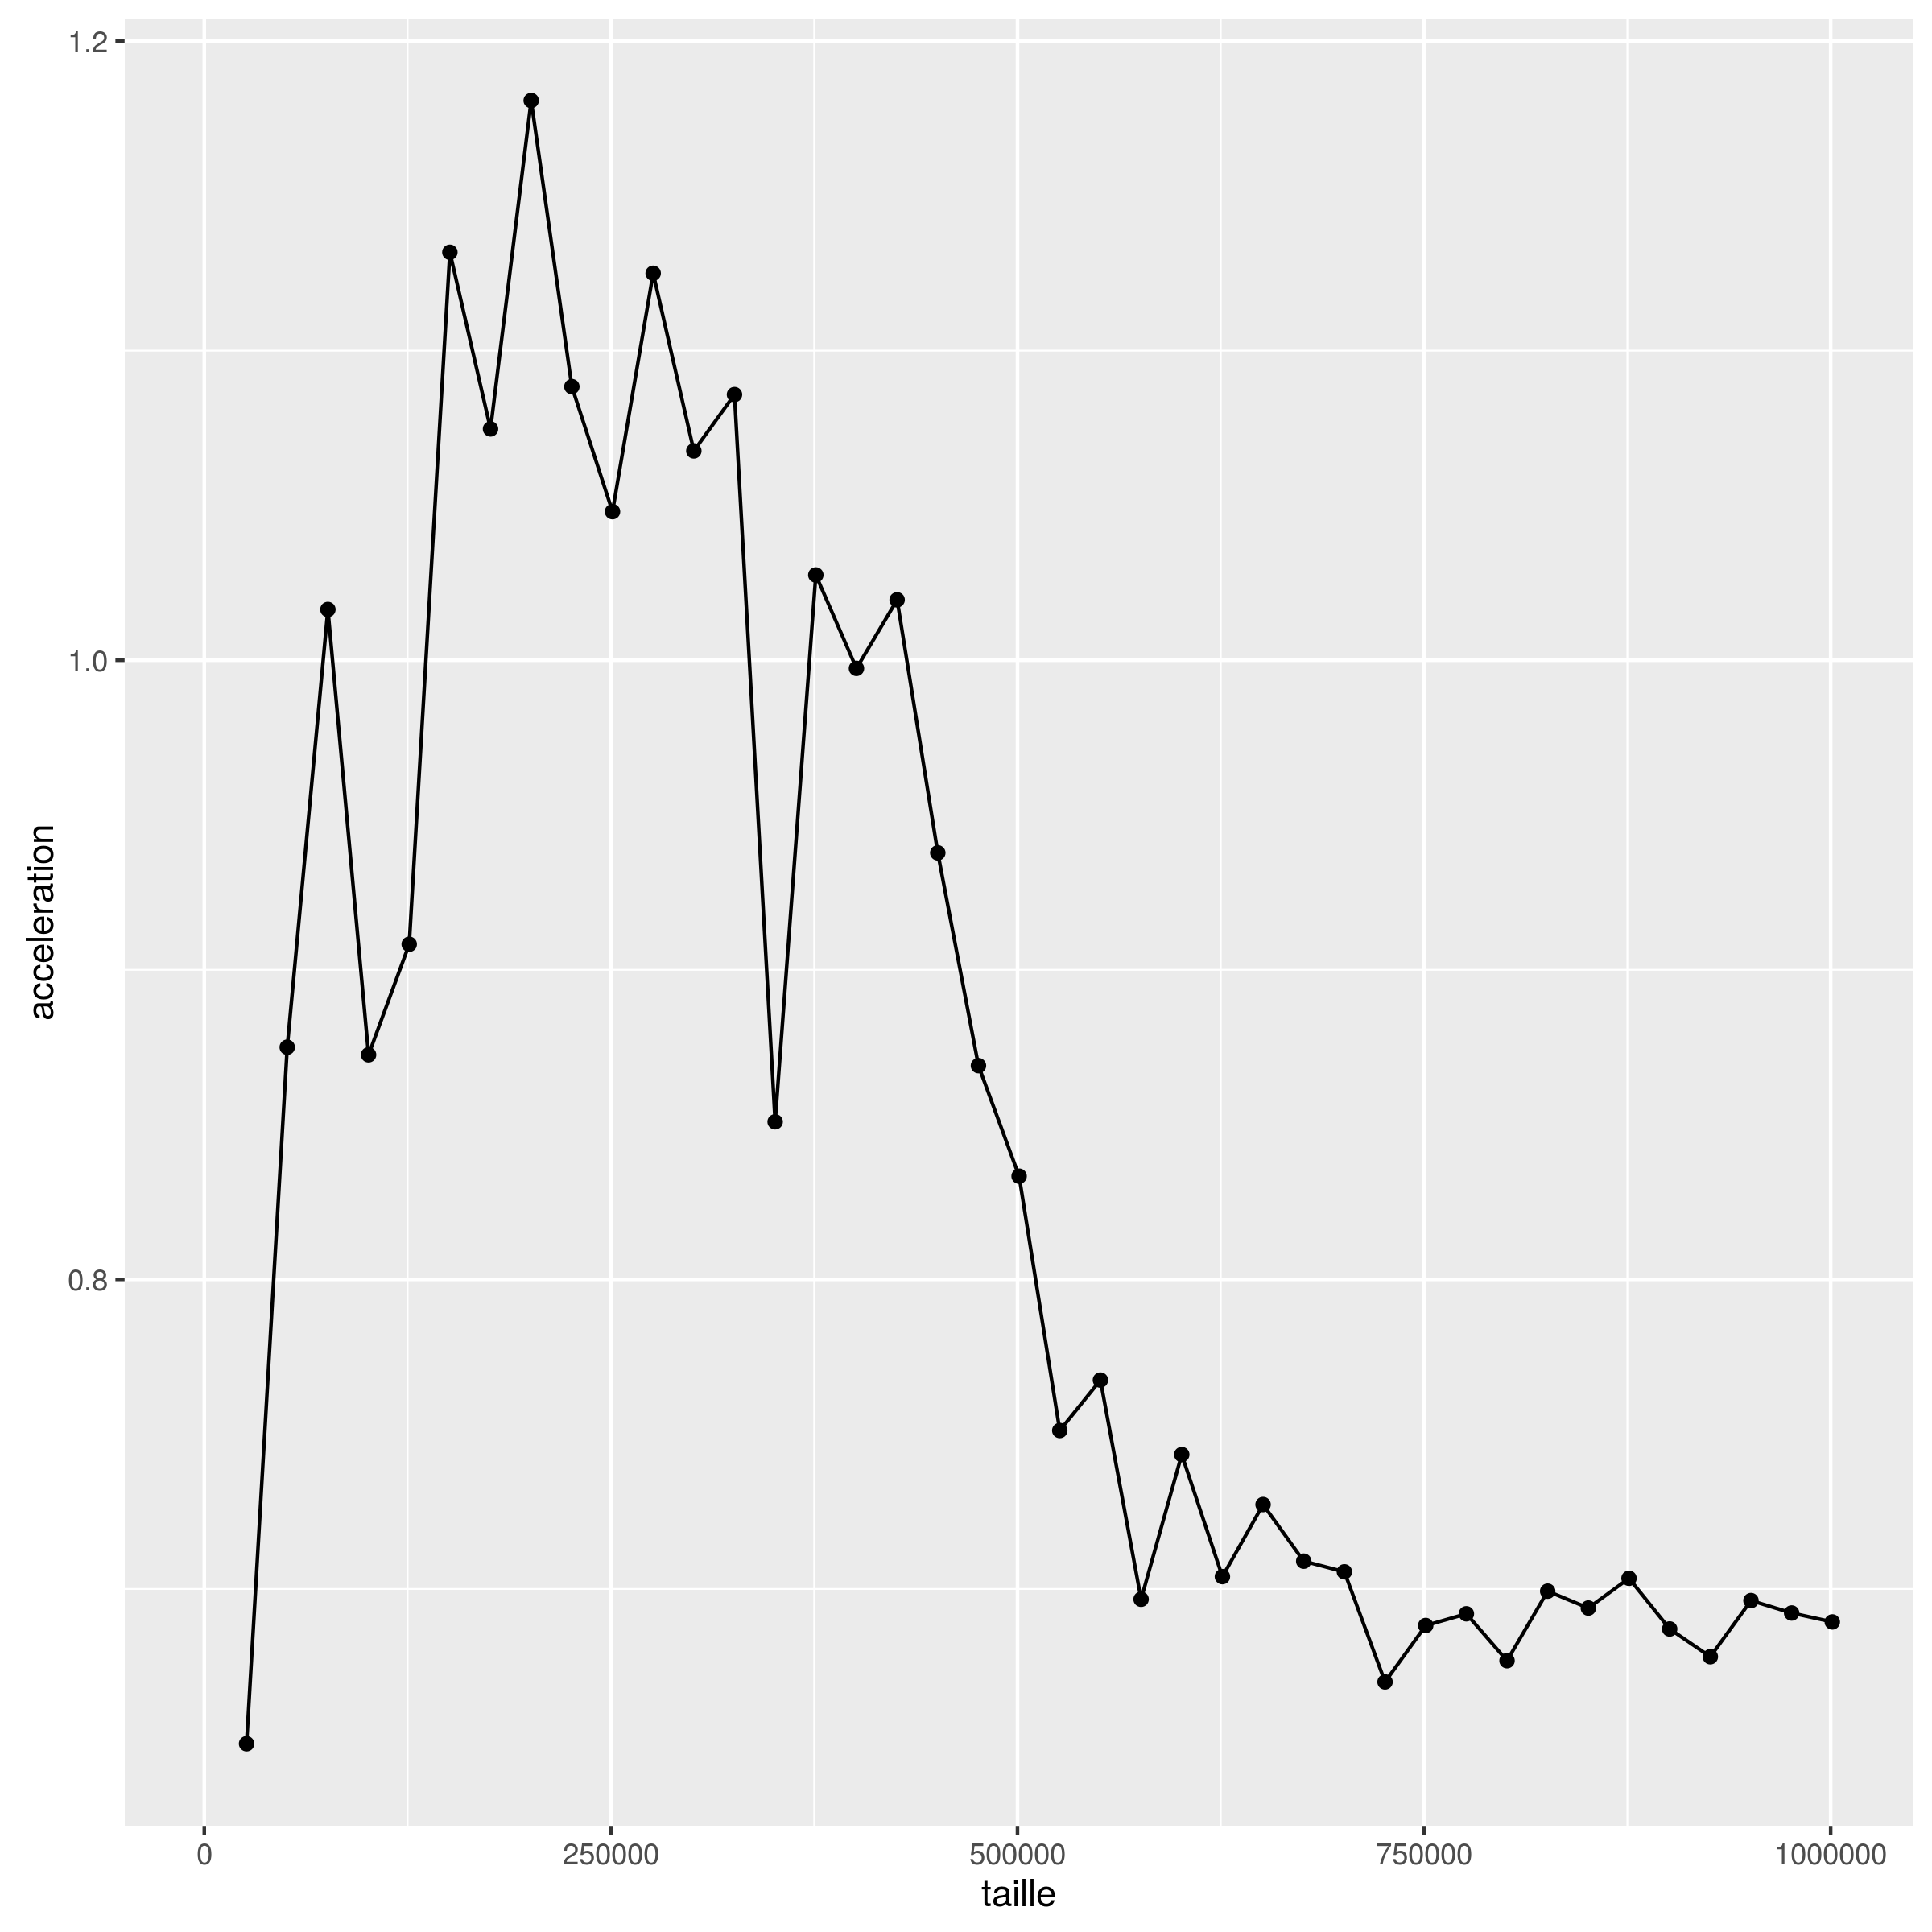
\includegraphics[scale=0.5] {graphes/temps_user_accel14.png}
\end{figure}
Nous observons que pour des vecteurs d'une taille inf\'erieur \`a 450000 et sup\'erieur \`a 25000, l'acc\'el\'eration est sup\'erieur \`a 1. N\'eanmoins pass\'e ce seuil,  l'acc\'el\'eration est maintenant inf\'erieur \`a un, cela signifie que le temps CPU cumul\'e de l'utilisateur finit par \^{e}tre plus \'elev\'e avec 14 threads qu'en s\'equentiel. Cette acc\'el\'eration finit par tendre vers 0.7.


\section{Avec 15 threads}
\subsection{Temps d'ex\'ecution}

\begin{figure}[H] \center
   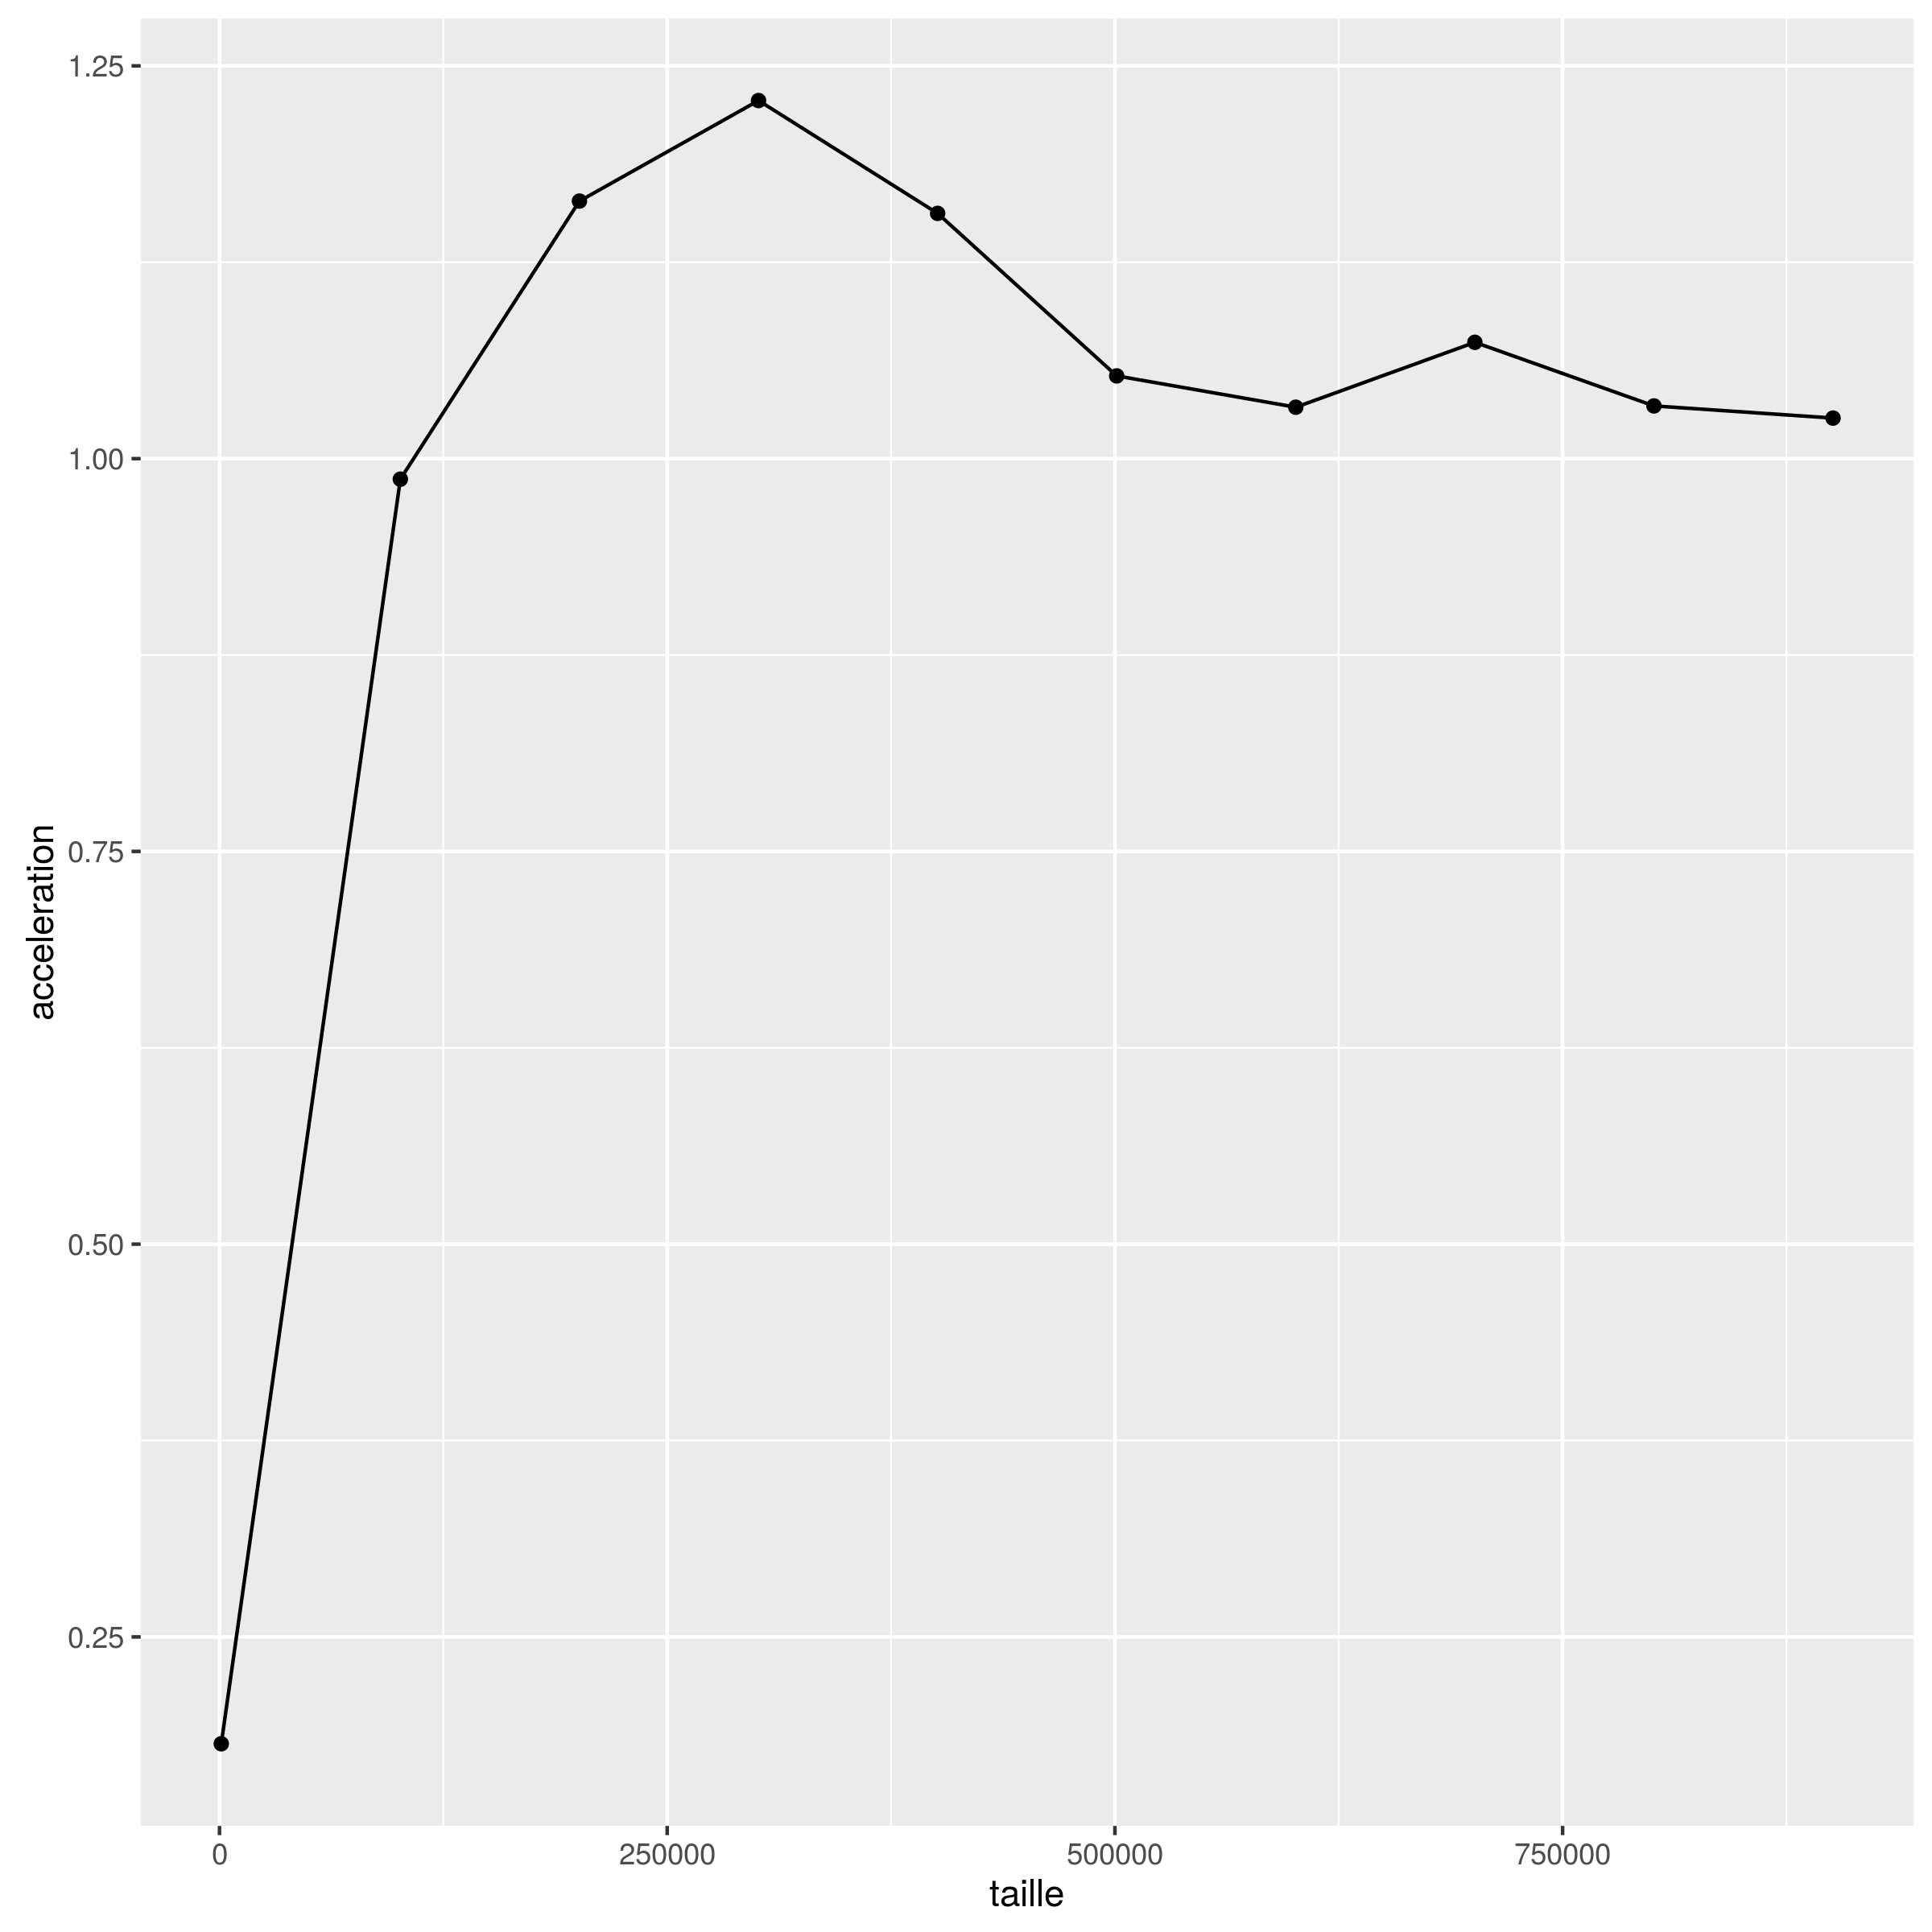
\includegraphics[scale=0.5] {graphes/global_temps_machine_accel15.png}
\end{figure}

Nous observons que pour des vecteurs allant d'une taille de 1000 \'el\'ements \`a 1000000 d'\'el\'ements, l'acc\'el\'eration est toujours sup\'erieur \`a 1. Nous observons aussi que l'acc\'el\'eration est la plus grande, pour des vecteurs d'une taille d'environ 400000 \'el\'ements. Pass\'e ce seuil, le niveau de l'acc\'el\'eration baisse et finit par tendre vers 1.2, pass\' le seuil des 500000 \'el\'ements.   


\subsection{Temps CPU cumul\'e de l'utilisateur}
\begin{figure}[H] \center
   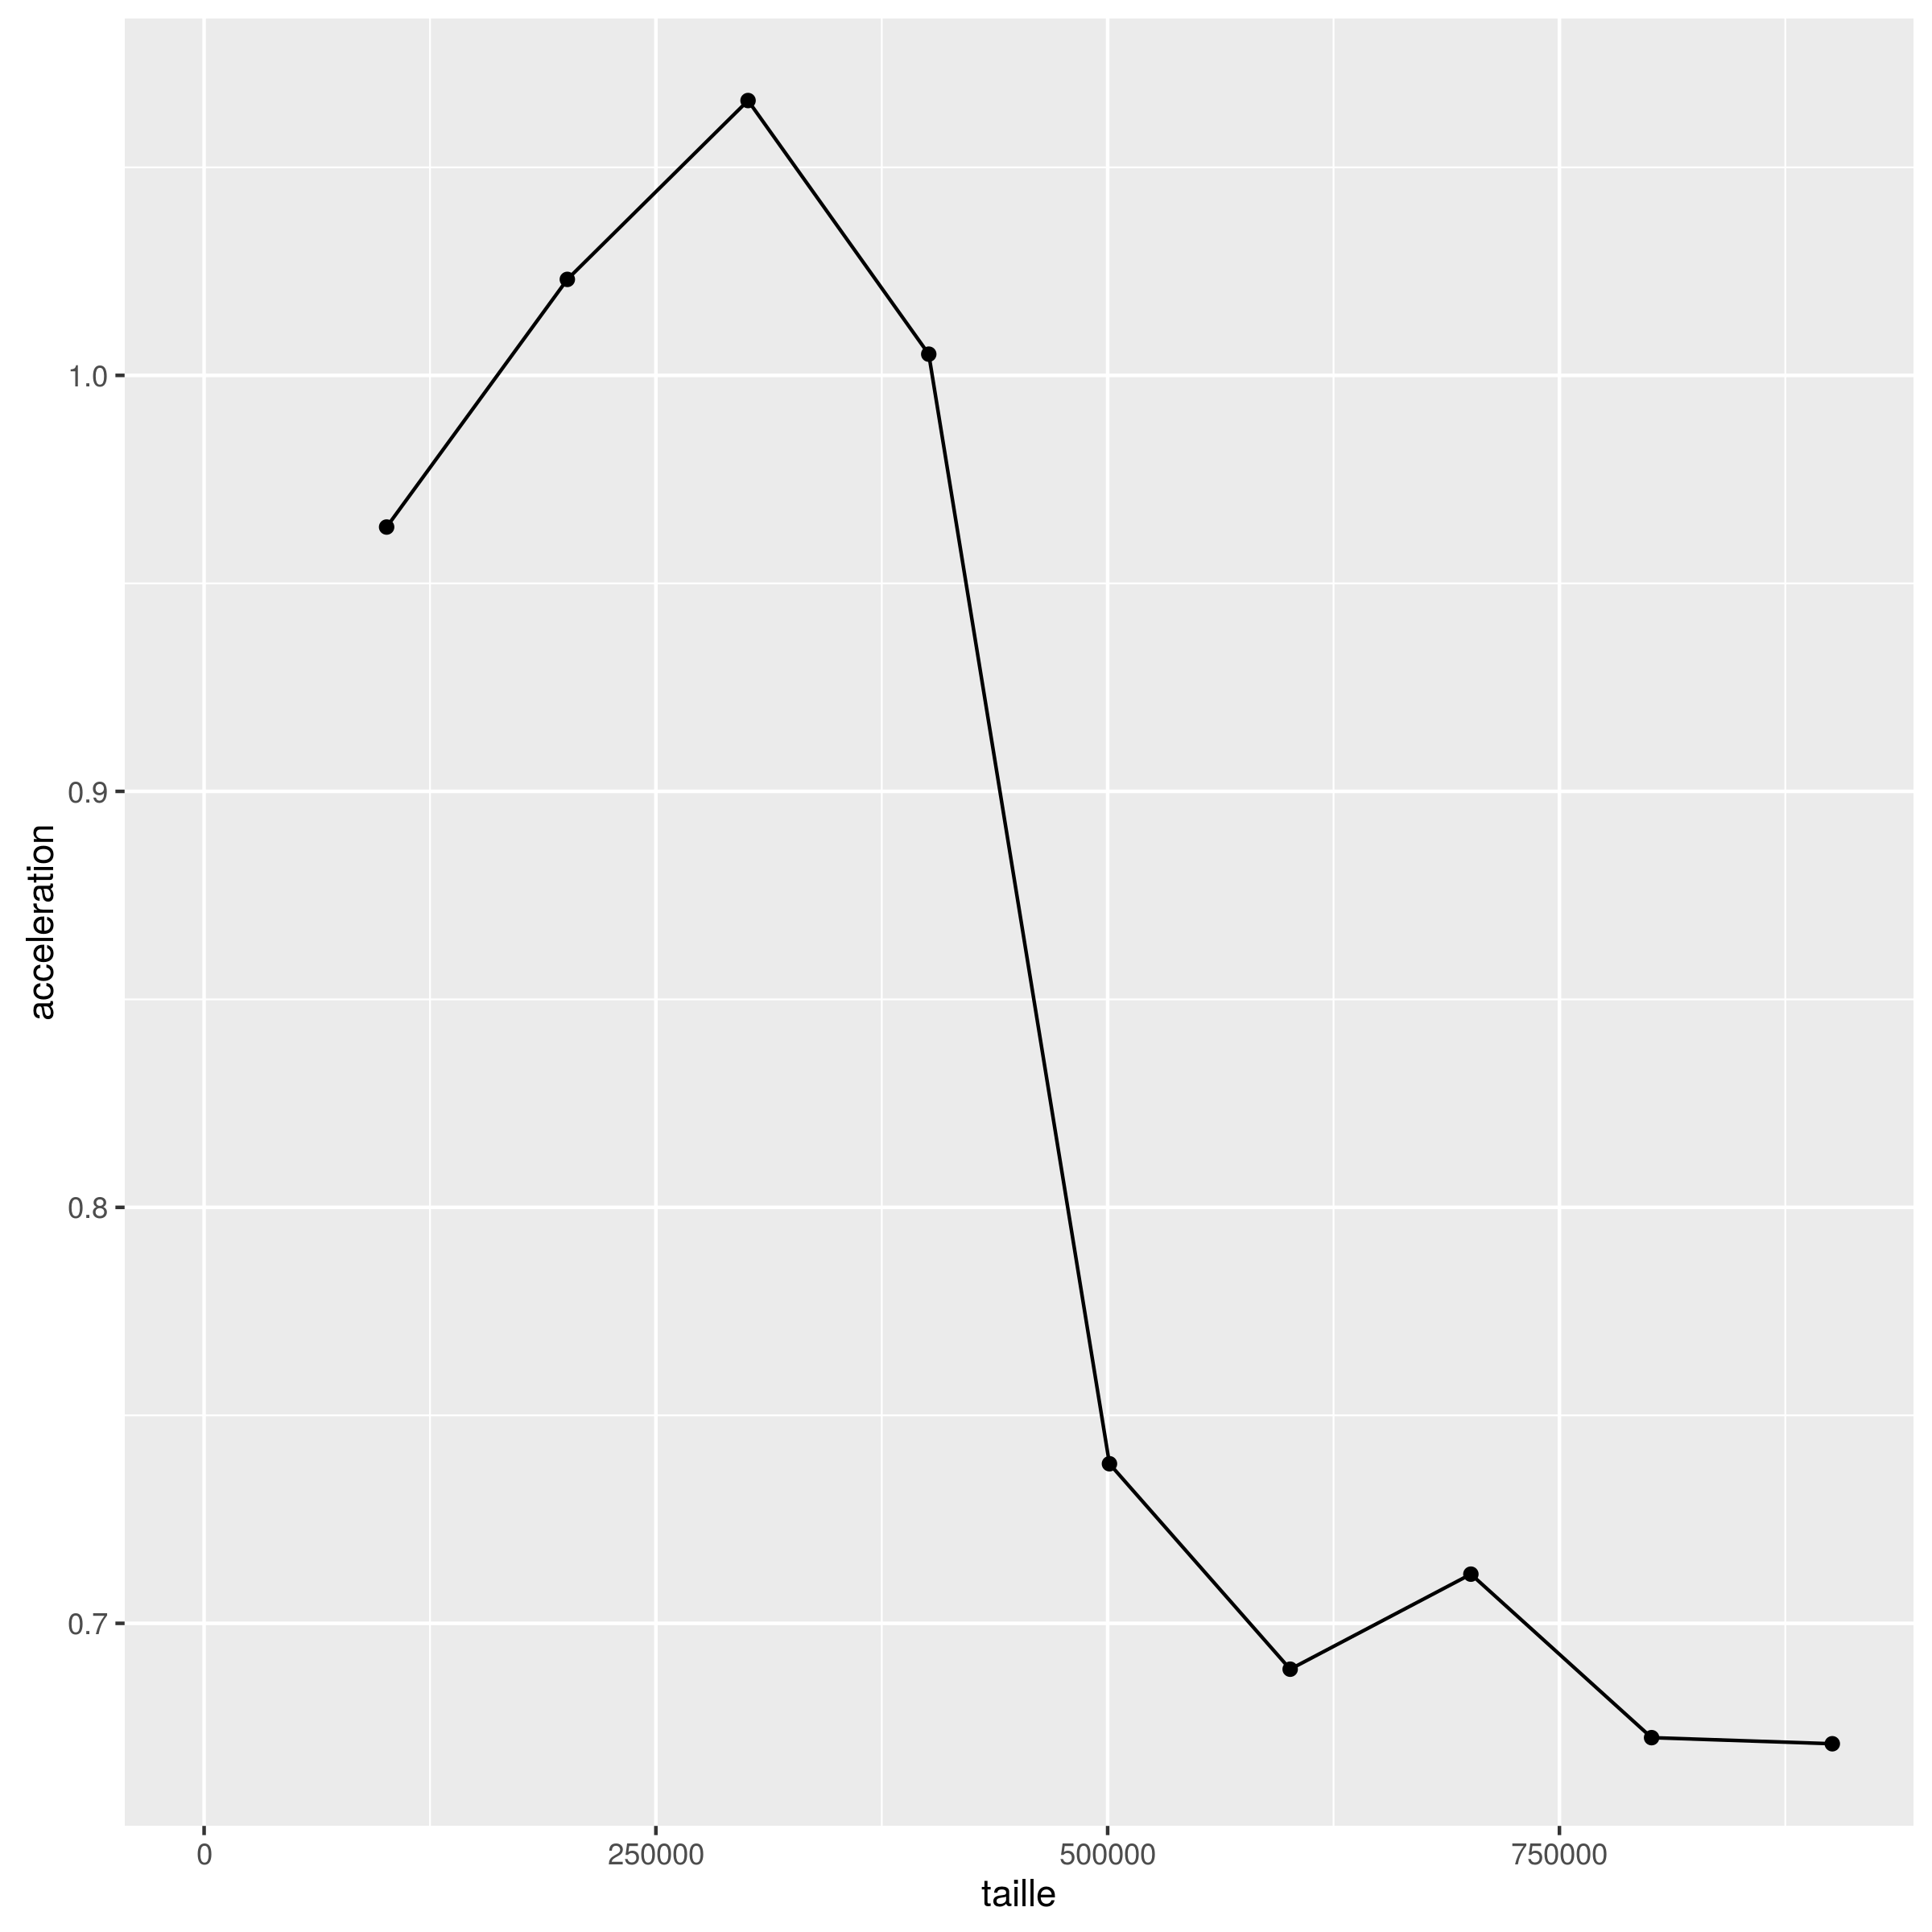
\includegraphics[scale=0.5] {graphes/temps_user_accel15.png}
\end{figure}
Nous observons que pour des vecteurs d'une taille inf\'erieur \`a 450000 et sup\'erieur \`a 25000, l'acc\'el\'eration est sup\'erieur \`a 1. N\'eanmoins pass\'e ce seuil,  l'acc\'el\'eration est maintenant inf\'erieur \`a un, cela signifie que le temps CPU cumul\'e de l'utilisateur finit par \^{e}tre plus \'elev\'e avec 15 threads qu'en s\'equentiel. Cette acc\'el\'eration finit par tendre vers 0.7.


\section{Avec 16 threads}
\subsection{Temps d'ex\'ecution}

\begin{figure}[H] \center
   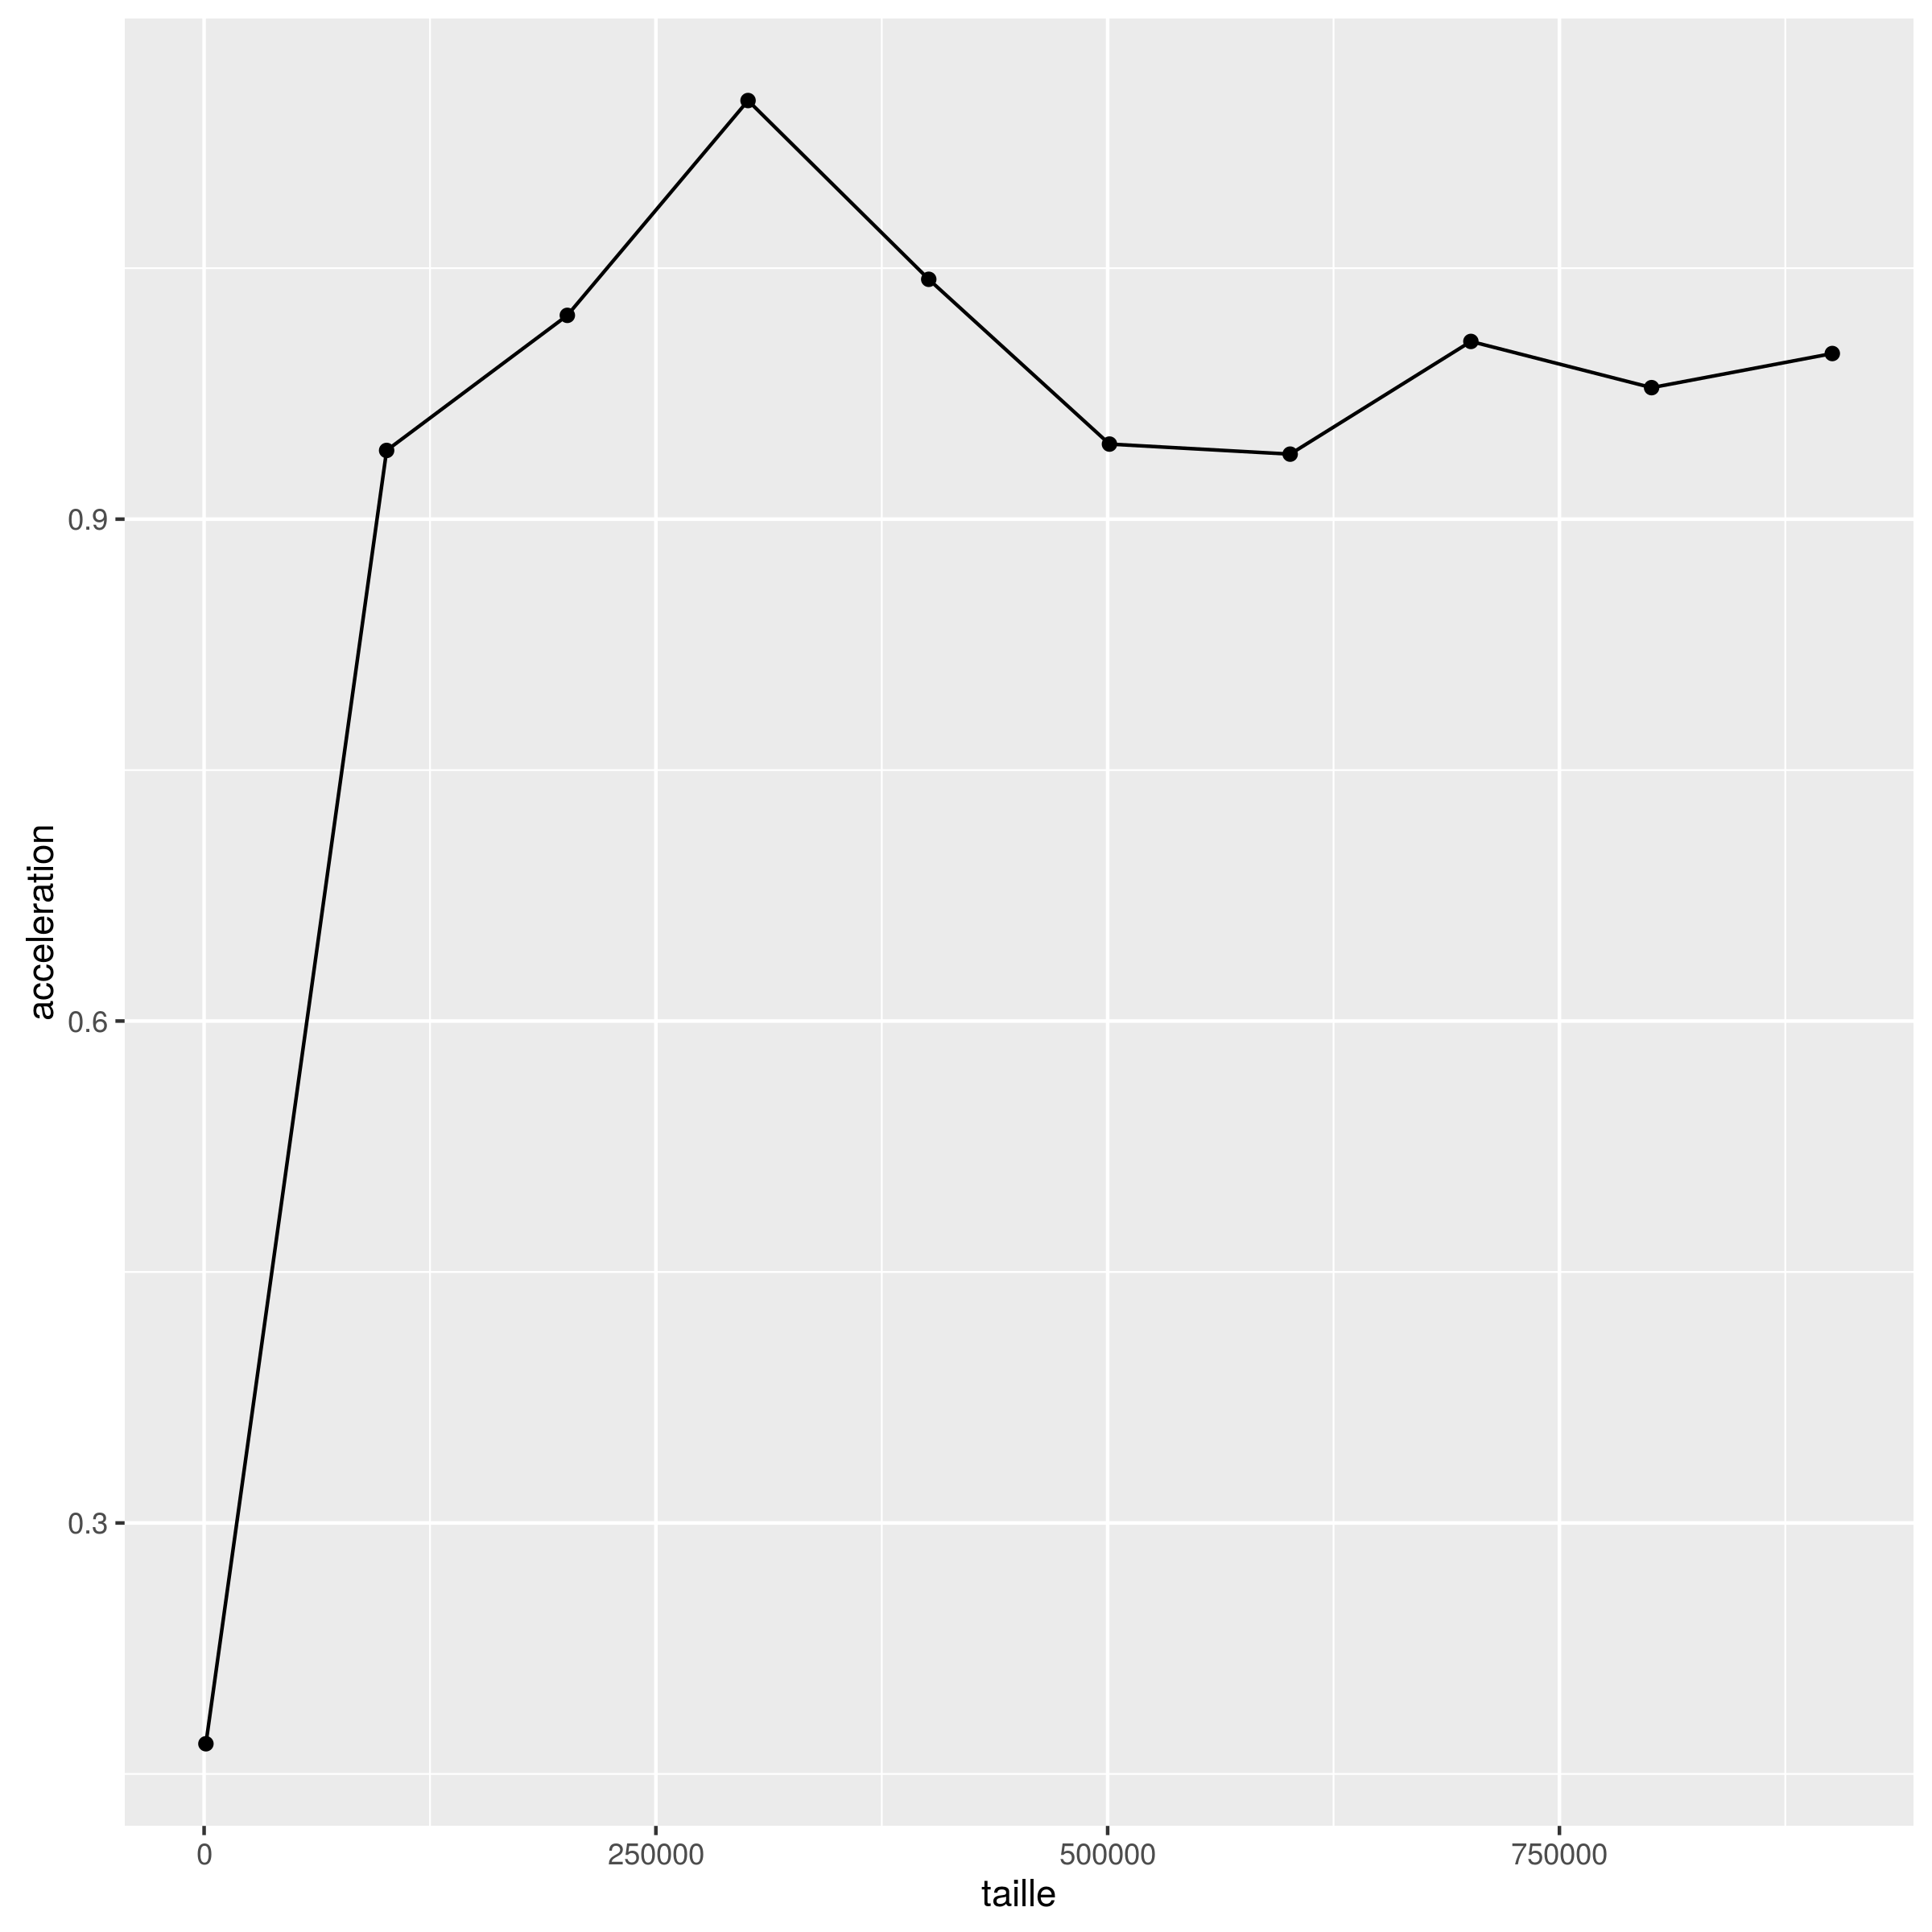
\includegraphics[scale=0.5] {graphes/global_temps_machine_accel16.png}
\end{figure}

Nous observons que pour des vecteurs allant d'une taille de 1000 \'el\'ements \`a 1000000 d'\'el\'ements, l'acc\'el\'eration est toujours inf\'erieur \`a 1. Nous observons aussi que l'acc\'el\'eration est la plus grande, pour des vecteurs d'une taille d'environ 300000 \'el\'ements. Pass\'e ce seuil, le niveau de l'acc\'el\'eration baisse et finit par tendre vers 0.95, pass\' le seuil des 500000 \'el\'ements.   


\subsection{Temps CPU cumul\'e de l'utilisateur}
\begin{figure}[H] \center
    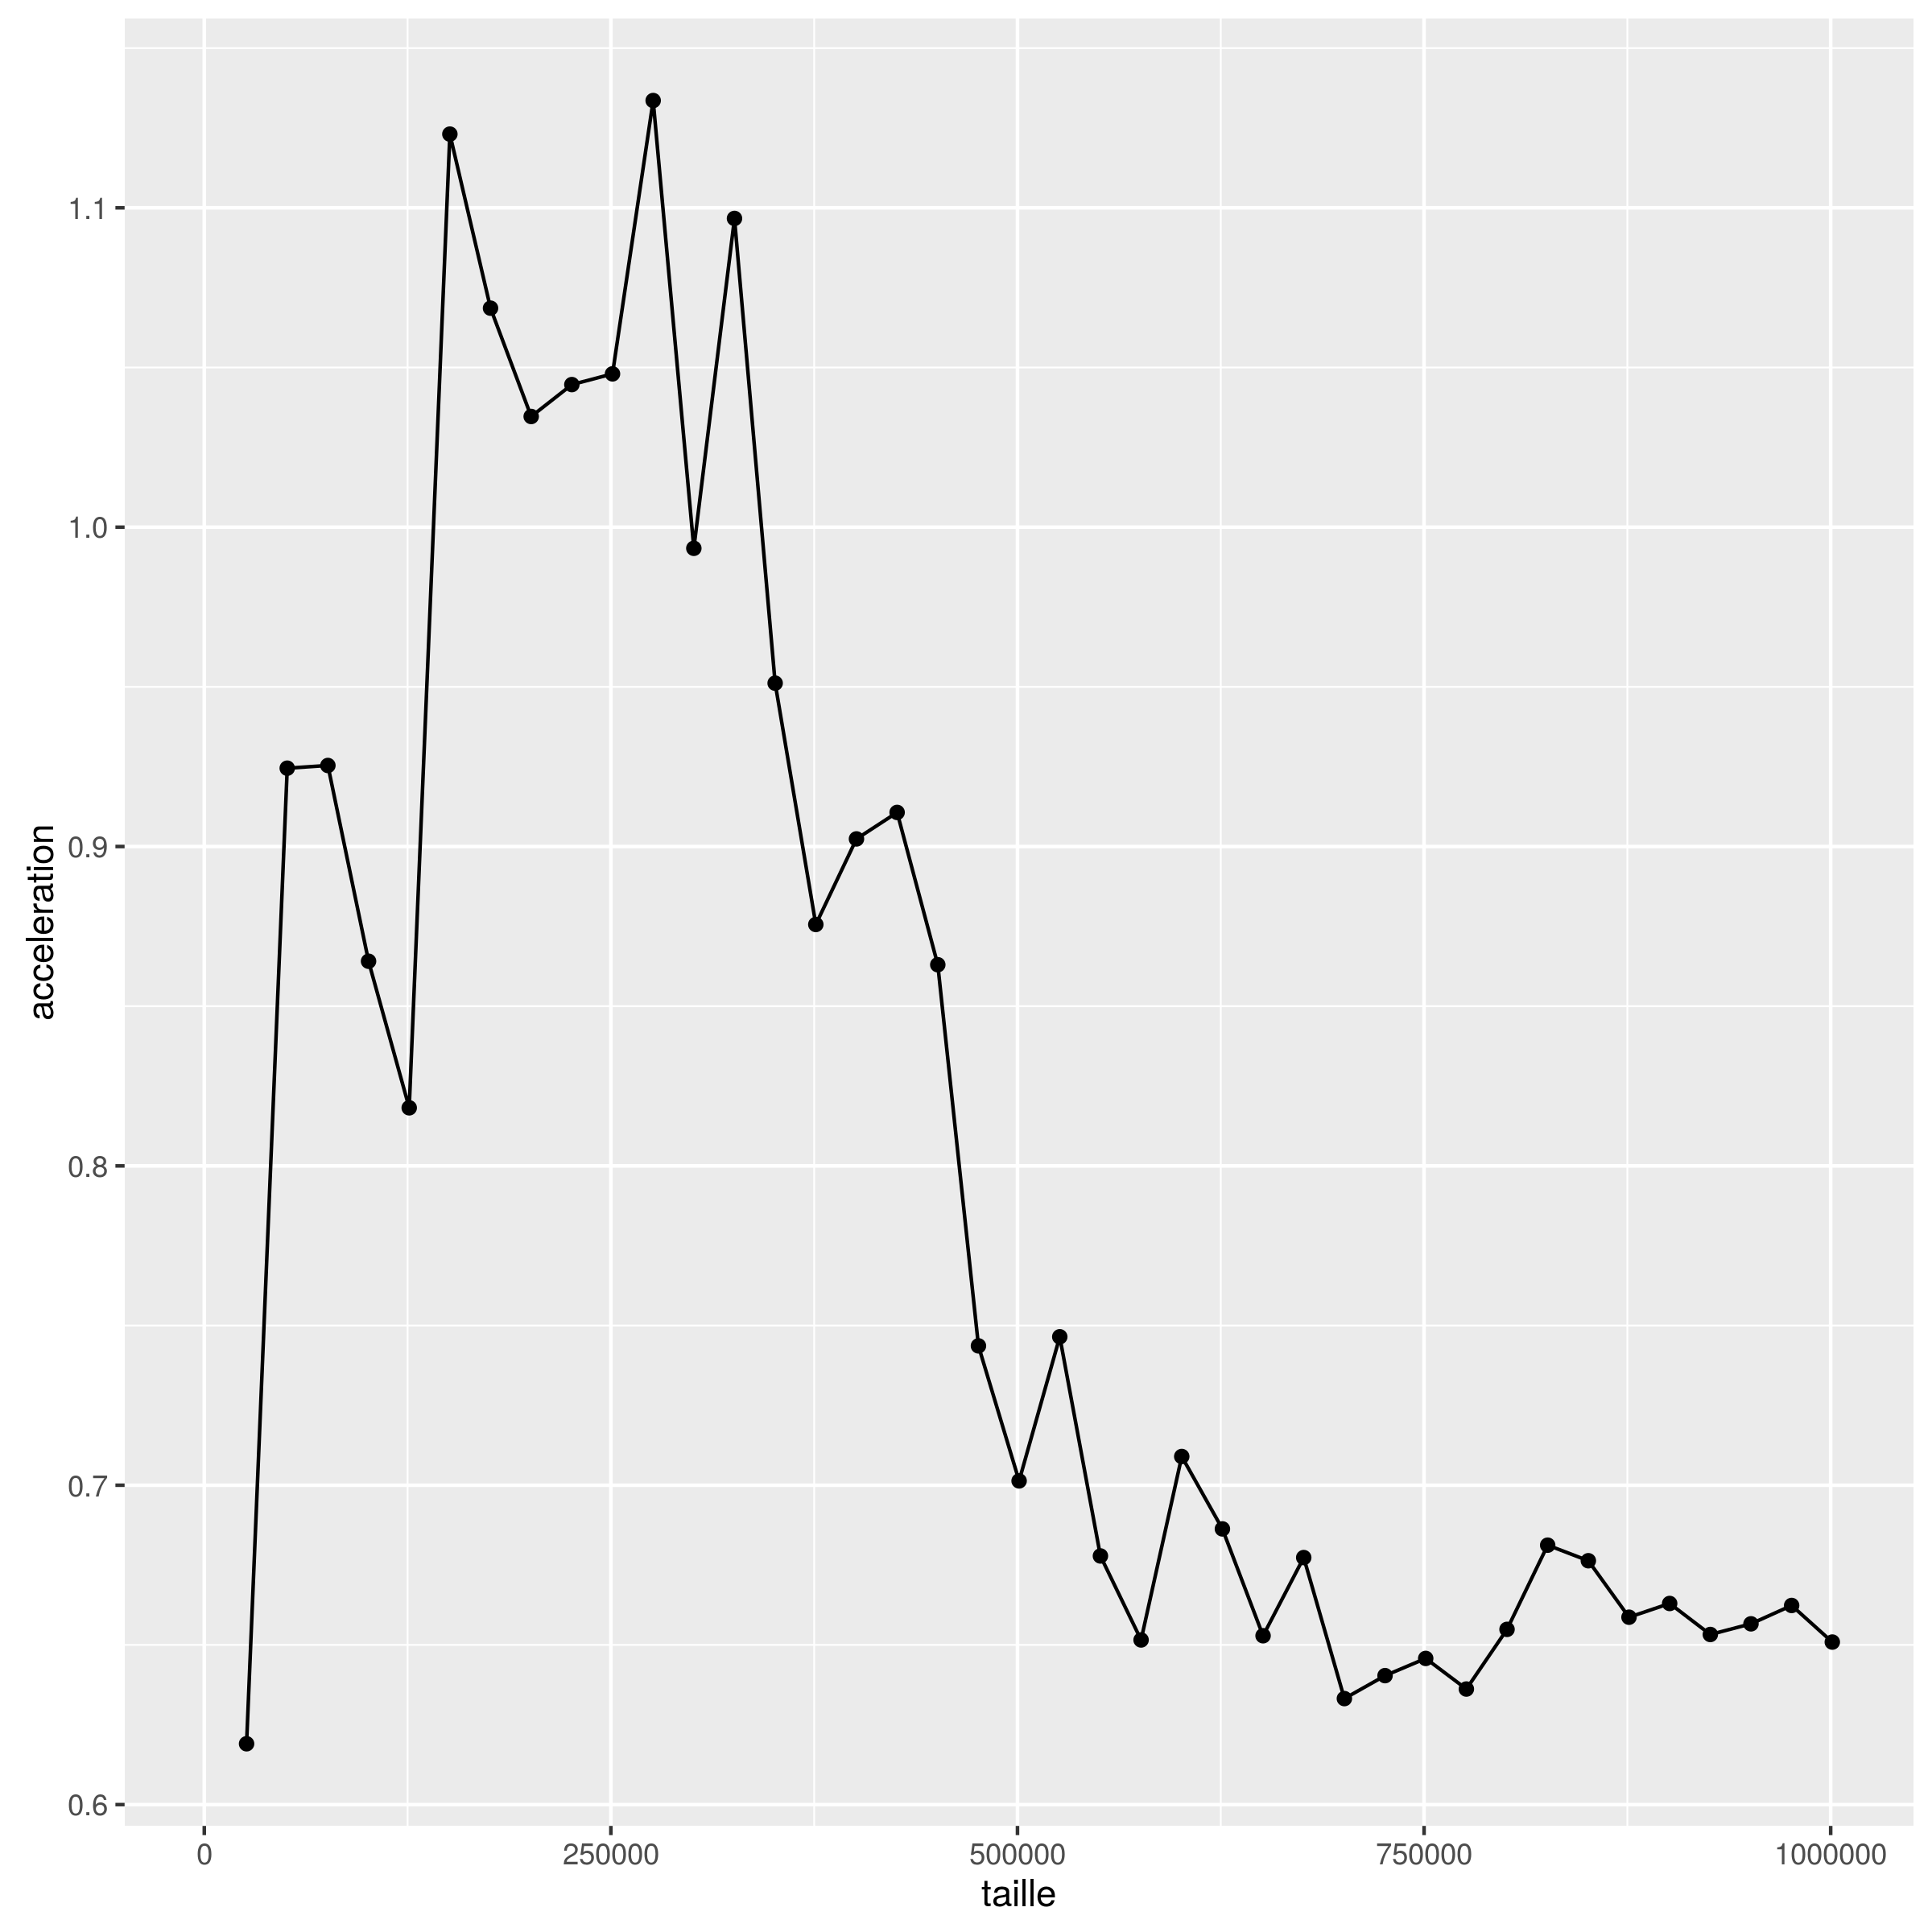
\includegraphics[scale=0.5] {graphes/temps_user_accel16.png}
\end{figure}
Nous observons que pour des vecteurs allant d'une taille de 1000 \'el\'ements \`a 1000000 d'\'el\'ements, l'acc\'el\'eration est toujours inf\'erieur \`a 1. Nous observons aussi que l'acc\'el\'eration est la plus grande, pour des vecteurs d'une taille d'environ 300000 \'el\'ements. Pass\'e ce seuil, le niveau de l'acc\'el\'eration baisse et finit par tendre vers 0.5, pass\' le seuil des 500000 \'el\'ements.

\section{Comparaison des r\'esultats}
\begin{figure}[H] \center
    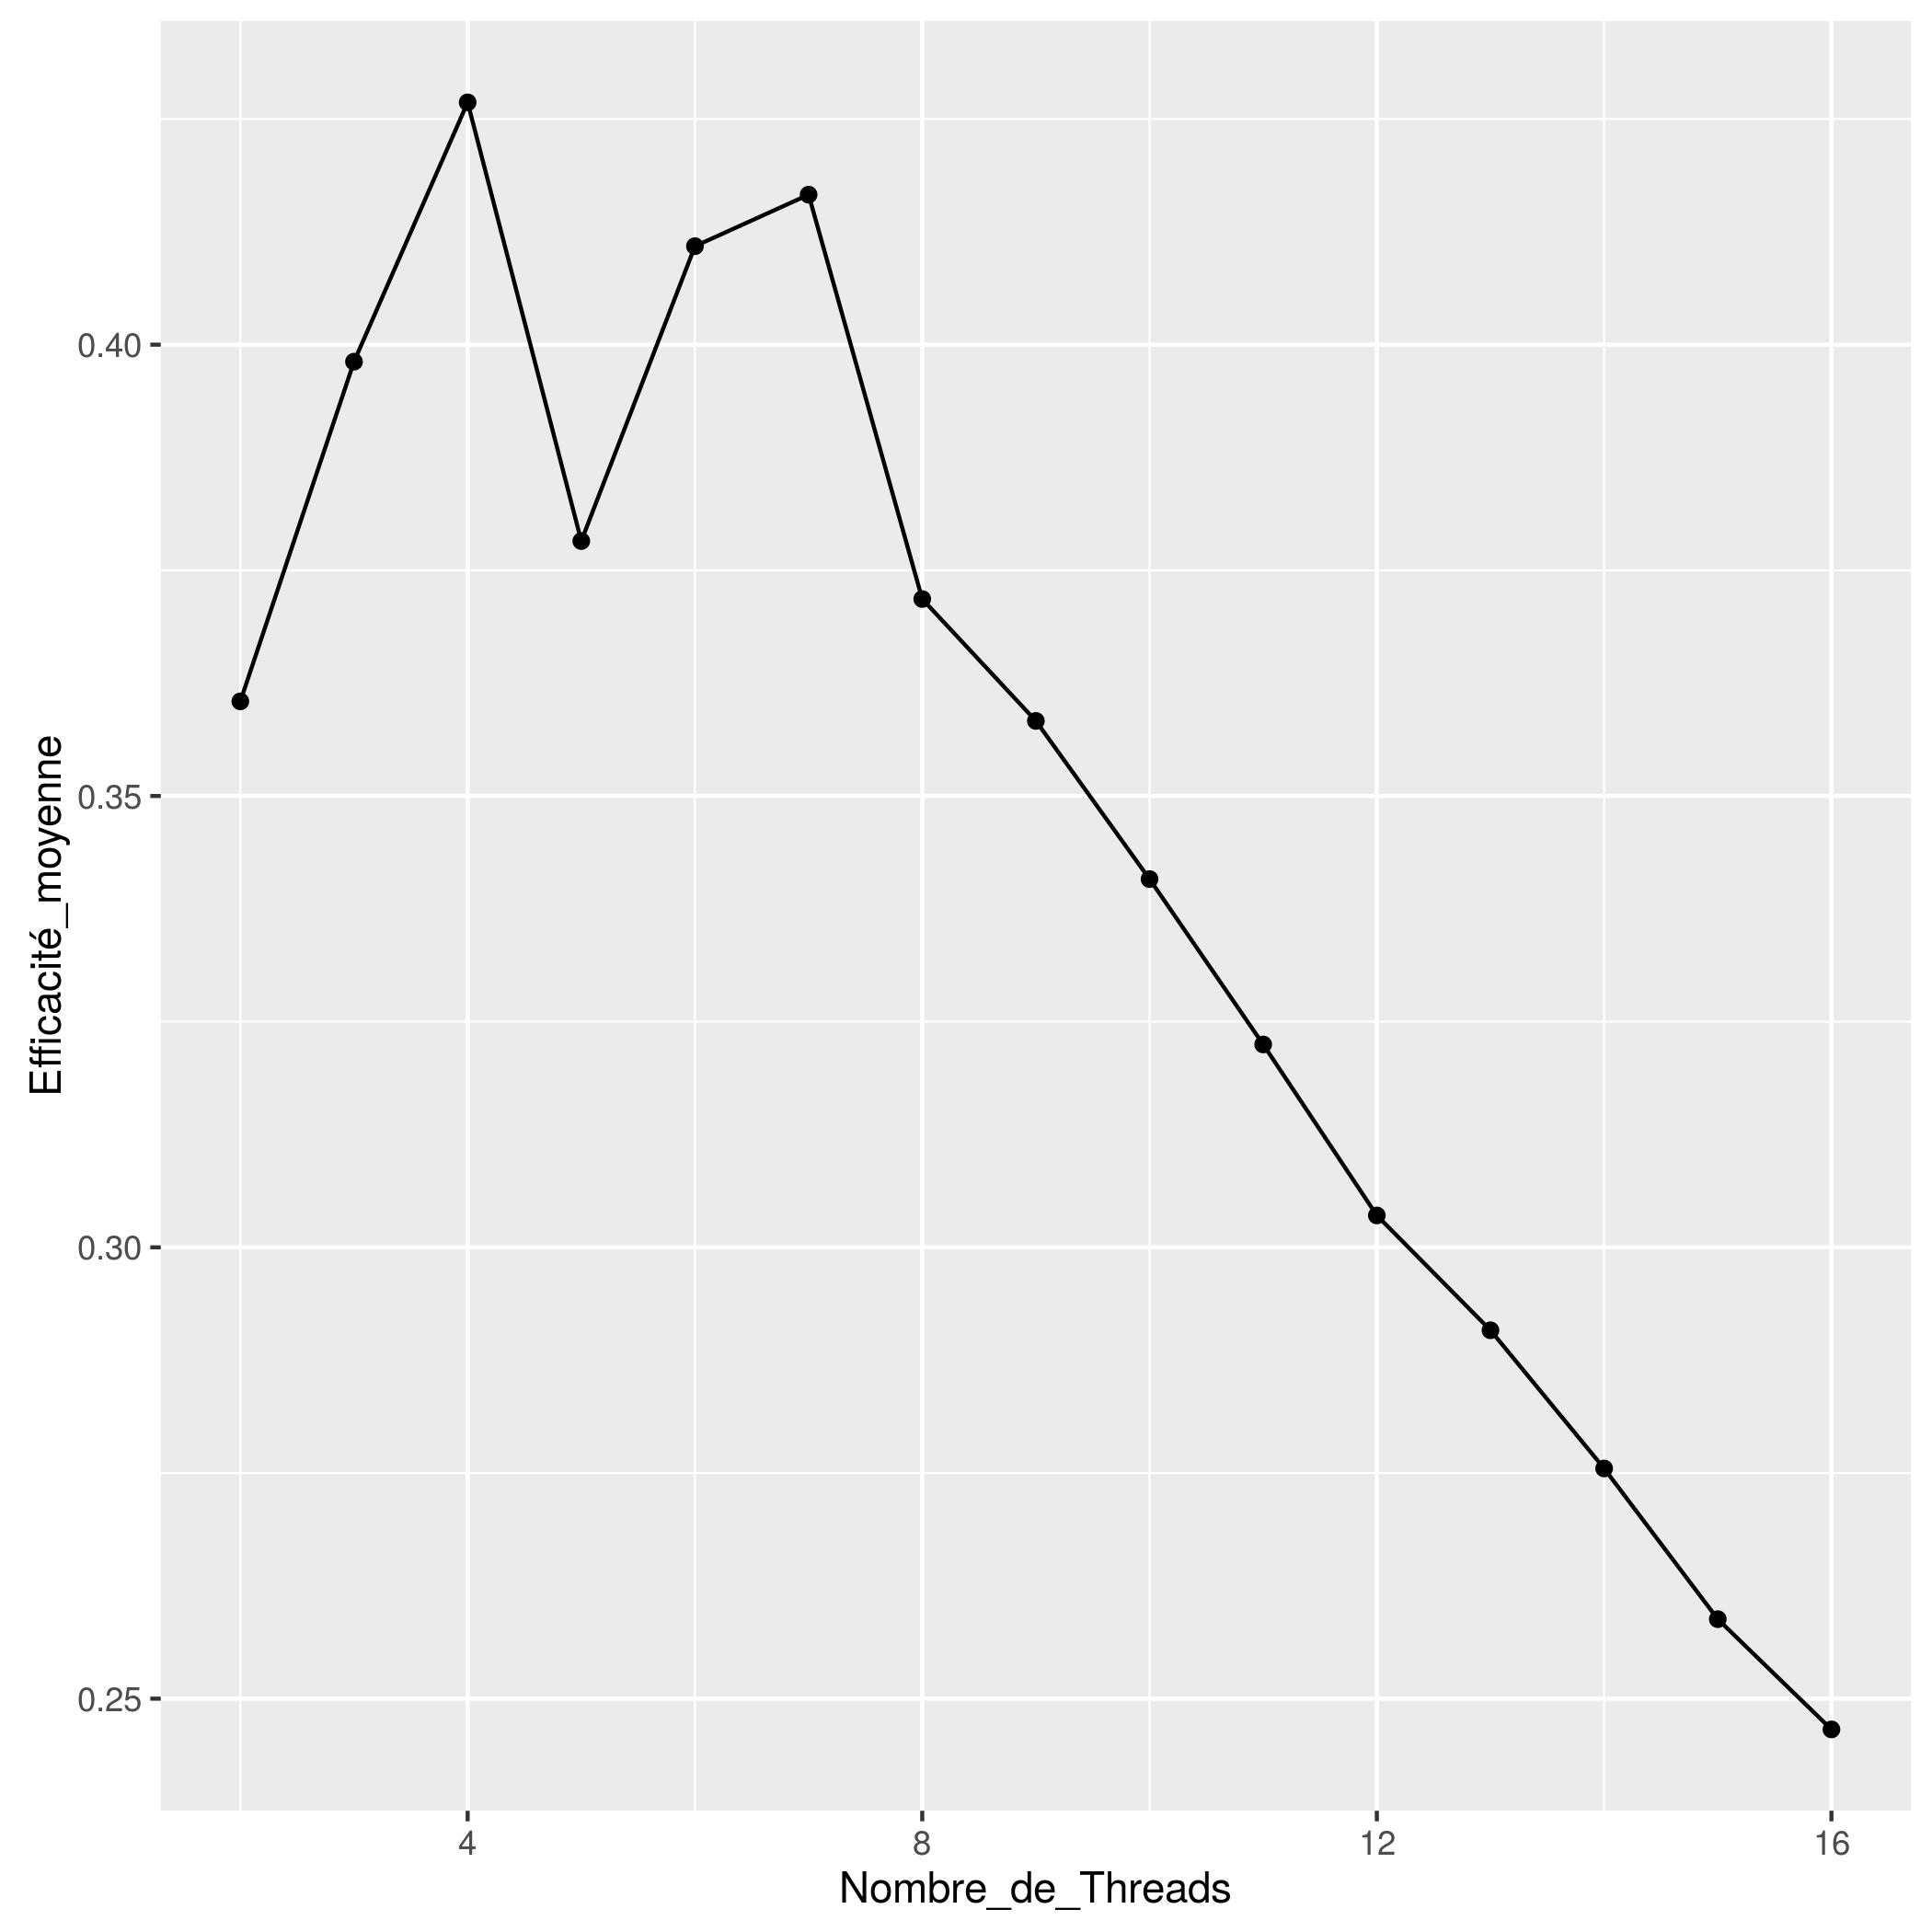
\includegraphics[scale=0.5] {graphes/compEff.png}
\end{figure}
Lorsque nous comparons l'efficacit\'e moyenne pour chaque version de l'algorithme paral\`elle, nus observons que le pic d'efficacit\'e est atteint pour 'algorithme avec 4 threads. Nous observons, qu'\`a partir de 5 threads, l'efficacit\'e baisse. 




\end{document}
